\documentclass[a4paper,12pt]{report}
\usepackage[font=small,labelfont=bf]{caption} 
\usepackage[headheight=150pt]{geometry}
\usepackage[square,numbers]{natbib}
\usepackage[portuguese]{babel}
\usepackage[nottoc]{tocbibind}
\usepackage[utf8]{inputenc}
\usepackage[T1]{fontenc}
\usepackage{amsmath}
\usepackage{caption}
\usepackage{enumitem}
\usepackage{fancyhdr}
\usepackage{float}
\usepackage{graphicx}
\usepackage{hyperref}
\usepackage{imakeidx}
\usepackage{listings}
\usepackage{indentfirst} 
\usepackage{lipsum}
\usepackage{pdfpages}
\usepackage{subcaption}
\usepackage{tikz}
\usepackage{color}

\definecolor{dkgreen}{rgb}{0,0.6,0}
\definecolor{gray}{rgb}{0.5,0.5,0.5}
\definecolor{mauve}{rgb}{0.58,0,0.82}
\lstset{ 
  language=Java,
  basicstyle=\footnotesize,
  stepnumber=1,
  numbersep=3pt,
  backgroundcolor=\color{white},
  showspaces=false,
  showstringspaces=false,
  showtabs=false,
  tabsize=2,
  captionpos=b,
  breaklines=true,
  breakatwhitespace=false,
  title=\lstname,
  keywordstyle=\color{blue},
  commentstyle=\color{dkgreen},
  stringstyle=\color{mauve},
  escapeinside={\%*}{*)},
  morekeywords={*,...}
}

\linespread{1.2}
\setlist[itemize]{noitemsep, topsep=0pt}
\pagestyle{fancy}
\bibliographystyle{unsrtnat}
\lhead{
\includegraphics[width=2cm]{img/ua.png}}
\rhead{Cláudio Henriques}
\title{
    \protect
\includegraphics[scale=0.8]{img/ua.png}\\
    [4cm]Trabalho 1\\
    Seminário de Matemática Aplicada
}

\author{
    Cláudio Henriques\\
    Mestrado em Matemática e Aplicações
}

\makeindex

\begin{document}

\maketitle
\tableofcontents
\listoffigures

\chapter{Introdução}

No presente relatório é apresentado o algoritmo desenvolvido para a coloração dos vértices de um determinado grafo, utilizando a sua matriz de adjacência para definir uma estrutura abstracta que o representa. É ainda apresentado um algoritmo de pesquisa em profundidade e uma proposta de resolução do exercício 3.

Por forma a auxiliar a construção dos algoritmos referidos anteriormente, foram desenvolvidas duas estruturas auxiliar para representar de forma abstrata um grafo e um vértice.

Estes algoritmos foram implementados recorrendo à linguagem de programação \textit{Java}. Foi ainda desenvolvido um pequeno script em \textit{R} para a visualização do grafo aplicando as colorações obtidas nos algoritmos.
Para a resolução do exercício 3 foi utilizado o \textit{software} \textit{Octave}.

\section{\textit{Java}}
A escolha da linguagem baseou-se essencialmente pelos recursos que esta oferece. Apesar de não ser tão rápida e consumir mais recursos computacionais quando comparada com o \textit{Python} ou \textit{Julia}, o \textit{Java} oferece um bom suporte para o desenvolvimento de algoritmos sob o velho conhecido paradigma \textit{Object-oriented programming (OOP)} (em português: Programação Orientada a Objetos (POO)).

A opção de implementar o trabalho em torno deste paradigma permite desenvolver \textit{módulos} que possam ser usados futuramente noutros trabalhos relacionados com esta temática. Um exemplo simples é poder usar a estrutura de dados abstrata criada para representar um grafo num outro trabalho/projeto em que seja necessário esta estrutura para desenvolver outro tipo de algoritmos. Assim permite a diminuição de código redundante (i.e. implementar várias vezes a mesma estrutura da dados sempre que necessitar de a utilizar em diferentes ambientes).

O facto de ter optado por esta linguagem permite também a adaptação das estruturas auxiliares criadas para auxiliar a construção dos algoritmos.

\section{Estruturas de Dados}
As estrturuas de dados desenvolvidas ao longo do projeto foram:
\begin{itemize}
    \item \textbf{Grafo} (\textit{Graph.java}): representar um objeto do tipo grafo (recorrendo à sua matriz de adjacência). Os atributos desta estrutura são:
    \begin{itemize}
        \item \textit{id} (identificador único do grafo);
        \item \textit{order} (ordem do grafo);
        \item \textit{vertexList} (lista de vértices do grafo);
    \end{itemize}
    Os métodos disponíveis são:
    \begin{itemize}
        \item \textit{getId ()} (retorna o \textit(id) do grafo);
        \item \textit{getOrder ()} (retorna a ordem do grafo);
        \item \textit{getVertexList ()} (retorna a lista de vértices do grafo);
        \item \textit{isNeighbor (int k, int y)} (retorna \textit{True} se o vértice k for vizinho de y ou \textit{False} no caso contrário);
        \item \textit{getVertexByDegree ()} (retorna a lista de vértices ordenada de forma crescente tendo em conta grau de cada um);
        \item \textit{sortVertexByDegree ()} (ordena a lista de vértices do grafo de forma crescente tendo em conta grau de cada um);
        \item \textit{setDefaultColorVertexes ()} (define todos os vértices com a cor 0);
    \end{itemize}
    \item \textbf{Vértice} (\textit{Vertex.java}):
    A estrutura anterior instancia uma estrutura auxiliar para representar cada vértice como um objeto único. Desta forma um grafo é representado com um conjunto de vértices.
    (Lógicamente seria óbvio representar um grafo como um conjunto de vértices e arestas, contudo as arestas (neste caso) não são estritamente necessárias ao desenvolvimento dos algoritmos, recorrendo apenas a atributos no objeto vértice para identificar os seus vizinhos). Os atributos do objeto são:
    \begin{itemize}
        \item \textit{id} (identificador único do vértice);
        \item \textit{color} (cor do vértice);
        \item \textit{order} (ordem do vértice);
        \item \textit{visited} (estado de visita do vértice);
        \item \textit{sucessorList} (lista de sucessores do vértice);
        \item \textit{predecessorList} (lista de predecessores do vértice);
    \end{itemize}
    Os métodos disponíveis são:
    \begin{itemize}
        \item \textit{getId ()} (retorna o id) do vértice);
        \item \textit{setColor (int color)} (define a cor do vértice);
        \item \textit{getColor ()} (retorna a cor do vértice);
        \item \textit{setOrder (int order)} (define a ordem do vértice);
        \item \textit{setVisited ()} (define o vértice como visitado);
        \item \textit{isVisited ()} (retorna \textit{True} se o vértice já foi visitado ou \textit{False} no caso contrário);
        \item \textit{setNeighbors (int k, int ps)} (define o vértice como vizinho do vértice k);
        \item \textit{isNeighbor ()} (retorna \textit{True} se o vértice é vizinho do vértice k ou \textit{False} no caso contrário);
        \item \textit{getNeighborList ()} (retorna a lista de vizinhos do vértice);
        \item \textit{getSucessorList ()} (retorna a lista de sucessores do vértice);
        \item \textit{getPredecessorList ()} (retorna a lista de predecessores do vértice);
        \item \textit{getDegree ()} (retorna o grau do vértice);
    \end{itemize}
\end{itemize}

\section{Algoritmos}
Os algoritmos desenvolvidos são:
\begin{itemize}
    \item \textbf{Coloração dos vértices, versão 1} (\textit{ColorizeVersion1.java}):
    Implementa o algoritmo apresentado nas aulas para a coloração dos vértices de um grafo, recorrendo à sua matriz de adjacência. Retorna a coloração obtida.
    \item \textbf{Coloração dos vértices, versão 2} (\textit{ColorizeVersion2.java}):
    Implementadado como uma extensão da versão 1 deste algoritmo, altera apenas a ordem pela qual percorre os vértices do grafo. Retorna a coloração obtida.
    \item \textbf{Coloração dos vértices, versão 3} (\textit{ColorizeVersion3.java}): Organiza os vértices pela ordem de maior grau, sendo este o critério para os percorrer e atribuir uma cor. Retorna a coloração obtida.
    \item \textbf{\textit{Depth First Search} (DFS)} (\textit{DFS.java}): Implementa o algoritmo para percorrer os vértices. Retorna a lista de vértices e a ordem pela qual foram visitados.
\end{itemize}

\section{Módulos extra}
Foi criado um módulo extra para o auxílio da construção de ficheiros \textit{*.txt}. Este mecanismo permite efetuar o \textit{debug} dos algoritmos, ou seja, permite verificar a cada passo onde é que o algoritmo pode estar a falhar.

Estes ficheiros podem também ser utilizados para uma melhor compreensão dos algoritmos.

\begin{itemize}
    \item \textbf{Ficheiro de logs} \textit{(WriteLogFile.java)} Os ficheiros criados através deste módulo são:
    \begin{itemize}
        \item\textit{log\_V1.txt};
        \item\textit{log\_V2.txt};
        \item\textit{log\_V3.txt};
        \item\textit{log\_dfs.txt};
    \end{itemize}
\end{itemize}

\chapter{Implementação}

Nesta secção é apresentada e explicada a implementação das estruturas de dados que foram desenvolvidas por forma a tornar os algoritmos mais eficientes.

Algumas linhas de código foram omitidas para simplificar a explicação, por exemplo, a implementação da criação do ficheiro auxiliar com a matriz de adjacência que vai ser lida pelo script \textit{R} uma vez que este processo não é essencial para o desenvolvimento dos algoritmos.
Foram também omitidas as linhas correspondentes à implementação dos ficheiros de \textit{log}.

Todo o código está comentado e pode ser visto em  \href{https://github.com/cfchenr/sma}{github.com/cfchenr/sma}.

\section{Grafo (\textit{Graph.java})}

Esta estrutura abstracta usa um \textit{ArrayList} para representar o conjunto de vértices pertencentes ao objeto grafo (denominada por \textit{vertexList}).

Cada grafo é identificado por um \textit{id} e contém um atributo chamado \textit{order} que representa a ordem do grafo.

\begin{lstlisting}[language=Java]
    private String id;
    private int order;
    private ArrayList<Vertex> vertexList;
\end{lstlisting}

Neste caso o \textit{id} é o nome do ficheiro com a matriz de adjacência que é lida. Por exemplo, se construir um grafo recorrendo à matriz de adjacência do ficheiro \textit{A.txt}, o \textit{id} deste grafo é definido como A.

\begin{lstlisting}
    id = file.split("/")[1].split("\\.")[0];
\end{lstlisting}

À medida que cada linha do ficheiro com a matriz de adjacência é lida, é adicinado à lista de vértices um novo vértice (pois cada linha da matriz identifica um vértice do grafo). Estes são identificados por um número que é igual à ordem do grafo na iteração anterior.

Por exemplo, se ainda não foi lida nenhuma linha então o primeiro vértice que é criado é representado por 0. Na linha seguinte é criado um novo vértice, desta vez já é representado pelo número 1.

Consequentemente a ordem do grafo é o número de linhas da matriz de adjacência.

\begin{figure}[H]
    \centering
        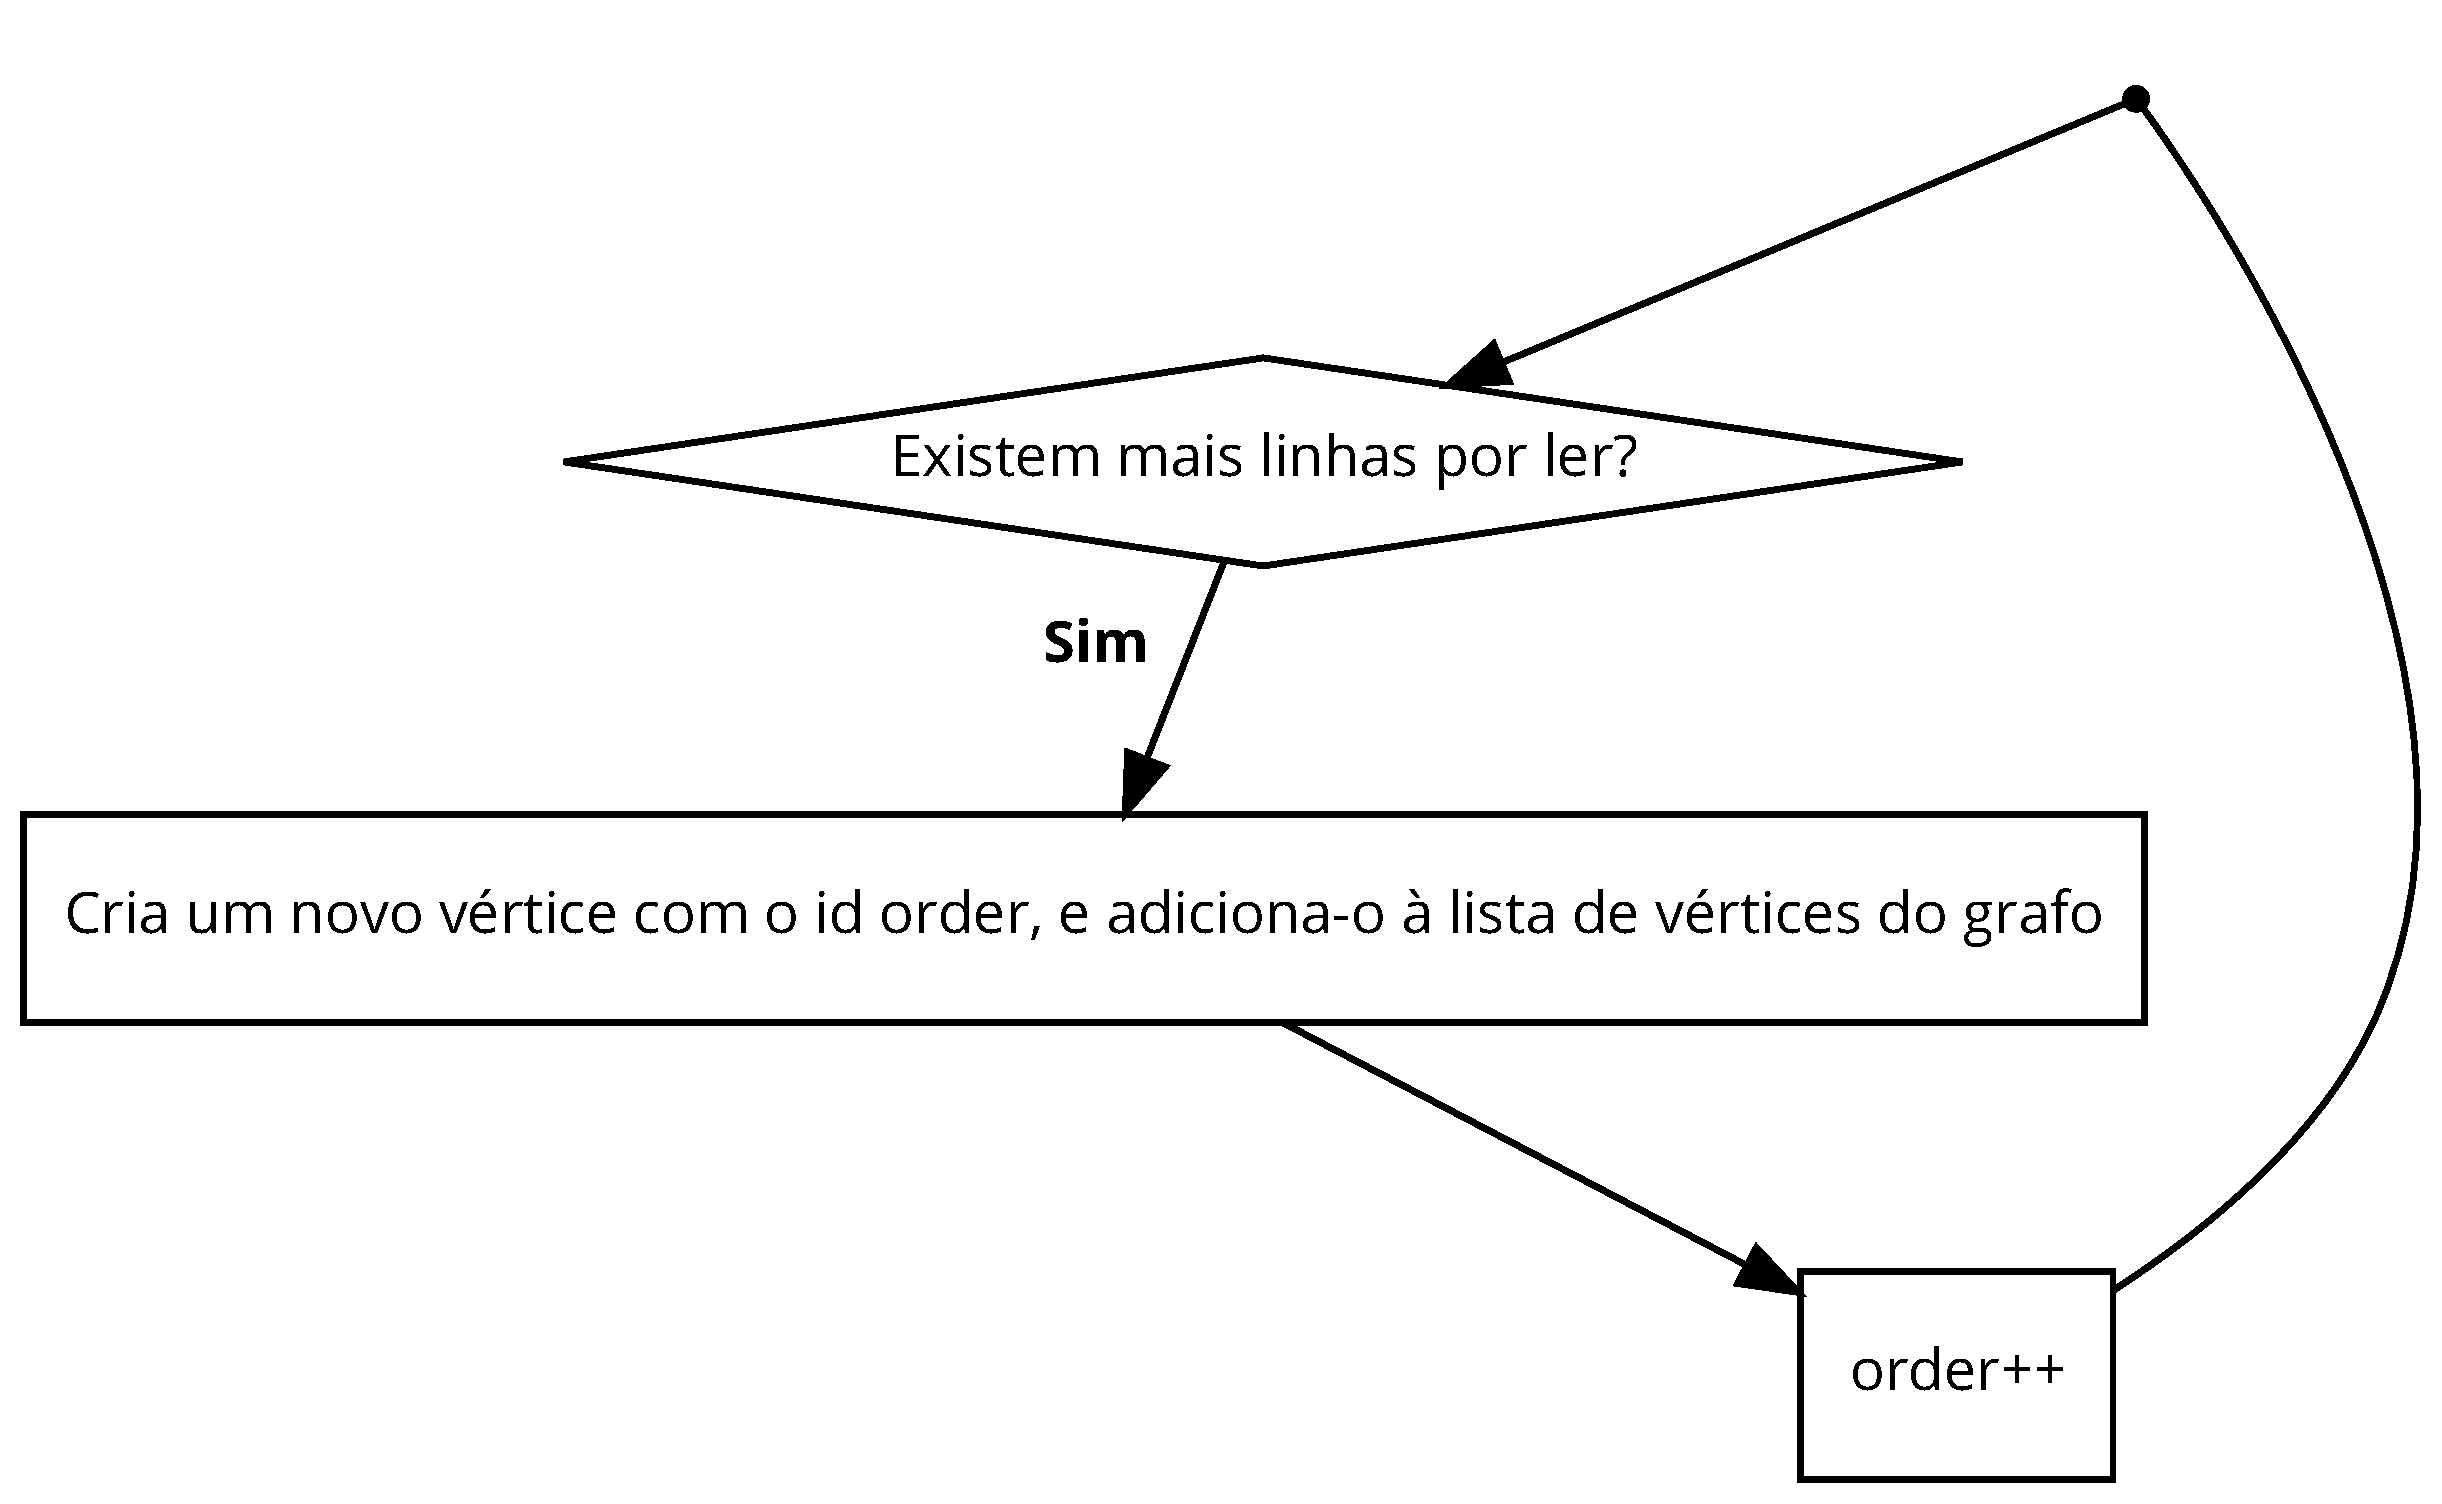
\includegraphics[scale=0.25]{img/lerLinhasDoFicheiro.pdf}
    \caption{Ler linhas do ficheiro}
    \label{fig:lldf}
\end{figure}

\begin{lstlisting}
    while (scf.hasNextLine()) {
        vertexList.add(new Vertex(order));       
        order++;
    }
\end{lstlisting}

Seguidamente são lidas cada uma das entradas de cada linha da matriz para se definir as vizinhanças de cada vértice. Desta forma, a cada entrada da linha que é lida, se for $1$ ou $-1$ então significa que o vértice que é representado pelo índice da linha da matriz é vizinho do vértice representado pelo índice da coluna da entrada em questão.

Consequentemente, se for $1$ então definimos que o vértice representado pelo índice da linha da matriz é sucessor do vértice representado pelo índice da coluna da entrada em questão. Lógicamente também definimos que o índice da coluna da entrada em questão é predecessor do vértice representado pelo índice da linha da matriz. (A distinção entre sucessor e predecessor é implementada na estrutura \textit{Vertex.java}, através da distinção do segundo argumento que é passado na função. Esta anotação é explicanda mais à frente na secção \ref{vertex}).

Analogamente utilizamos a mesma metodologia no caso da entrada ser $-1$.

\begin{figure}[H]
    \centering
        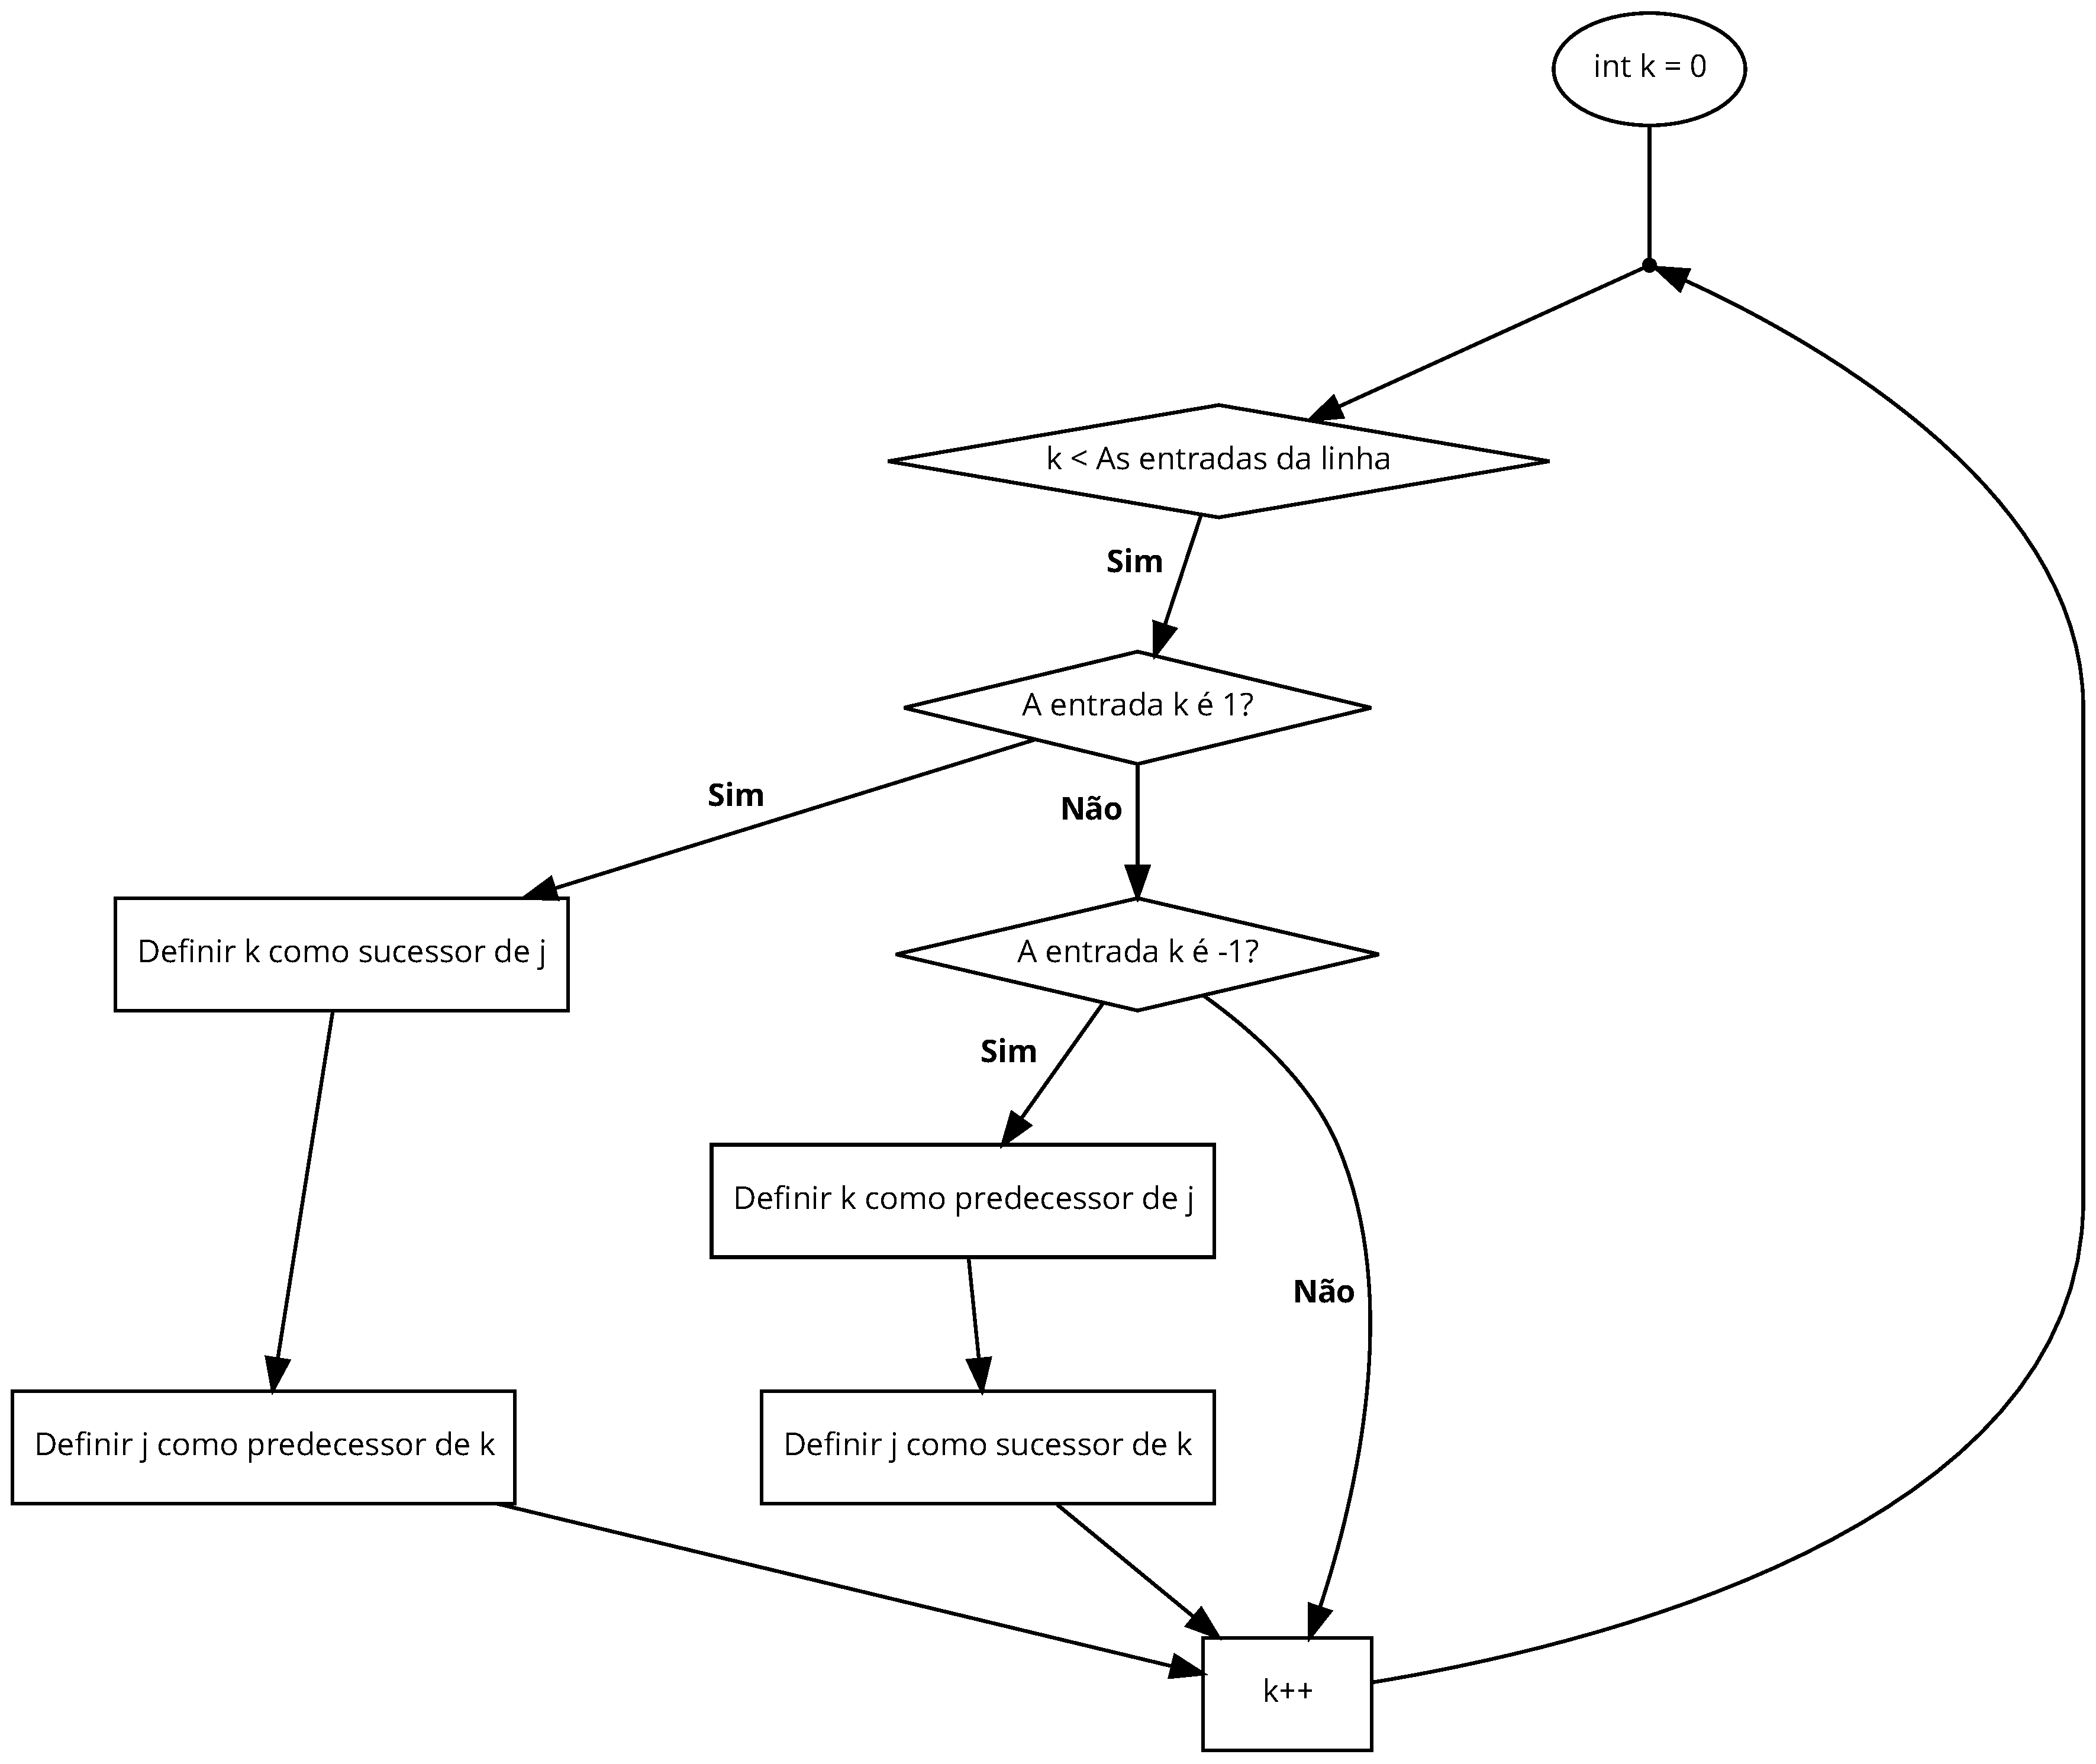
\includegraphics[scale=0.25]{img/definirSucessorEPredecessor.pdf}
    \caption{Definir sucessores e predecessores}
    \label{fig:dsep}
\end{figure}

\begin{lstlisting}
    for (int k = 0; k < line.length; k++) {
        if (line[k].equals("1")) {
            vertexList.get(j).setNeighbors(k, 1);
            vertexList.get(k).setNeighbors(j, -1);
        } else if (line[k].equals("-1")) {
            vertexList.get(j).setNeighbors(k, -1);
            vertexList.get(k).setNeighbors(j, 1);
        }
    }
\end{lstlisting}

O método \textit{getId ()} retorna o \textit{id} deste grafo.

\begin{lstlisting}
        return id;
\end{lstlisting}

O método \textit{getOrder ()} retorna a ordem do grafo.

\begin{lstlisting}
        return order;
\end{lstlisting}

O método \textit{getVertexList ()} retorna a lista com todos os vértices do grafo.

\begin{lstlisting}
        return vertexList;
\end{lstlisting}

O método \textit{isNeighbor (int k, int y)} retorna um valor booleano para dar resposta à pergunta "k é vizinho de y?". Reparemos que k ser vizinho de y é a mesma coisa que y ser vizinho de k.

\begin{lstlisting}
        return (vertexList.get(k).isNeighbor(y) || vertexList.get(y).isNeighbor(k));
\end{lstlisting}

O método \textit{getVertexByDegree ()} retorna uma lista de vértices por ordem crescente do grau do vértice.

Neste método é criada uma estrutura temporária para armazenar os vértices pela ordem pretendida.

Num primeiro momento, é obtido o grau máximo de todos os vértices. Após esta operação é adicionada à estrutura temporária os vértices que têm o grau igual ao grau máximo (os vértices são adicionamos sempre ao inicio da lista, o que permite criar a lista por ordem crescente de grau dos vértices). Quando não houver mais vértices com o grau máximo então é reduzido o valor máximo numa unidade voltando a efetuar o processo anterior. Este ciclo termina quando o valor máximo for 0.

Por fim é retornada a estrutura temporária, sendo esta uma lista com os vértices organizados por ordem crescente do grau.

\begin{figure}[H]
    \centering
        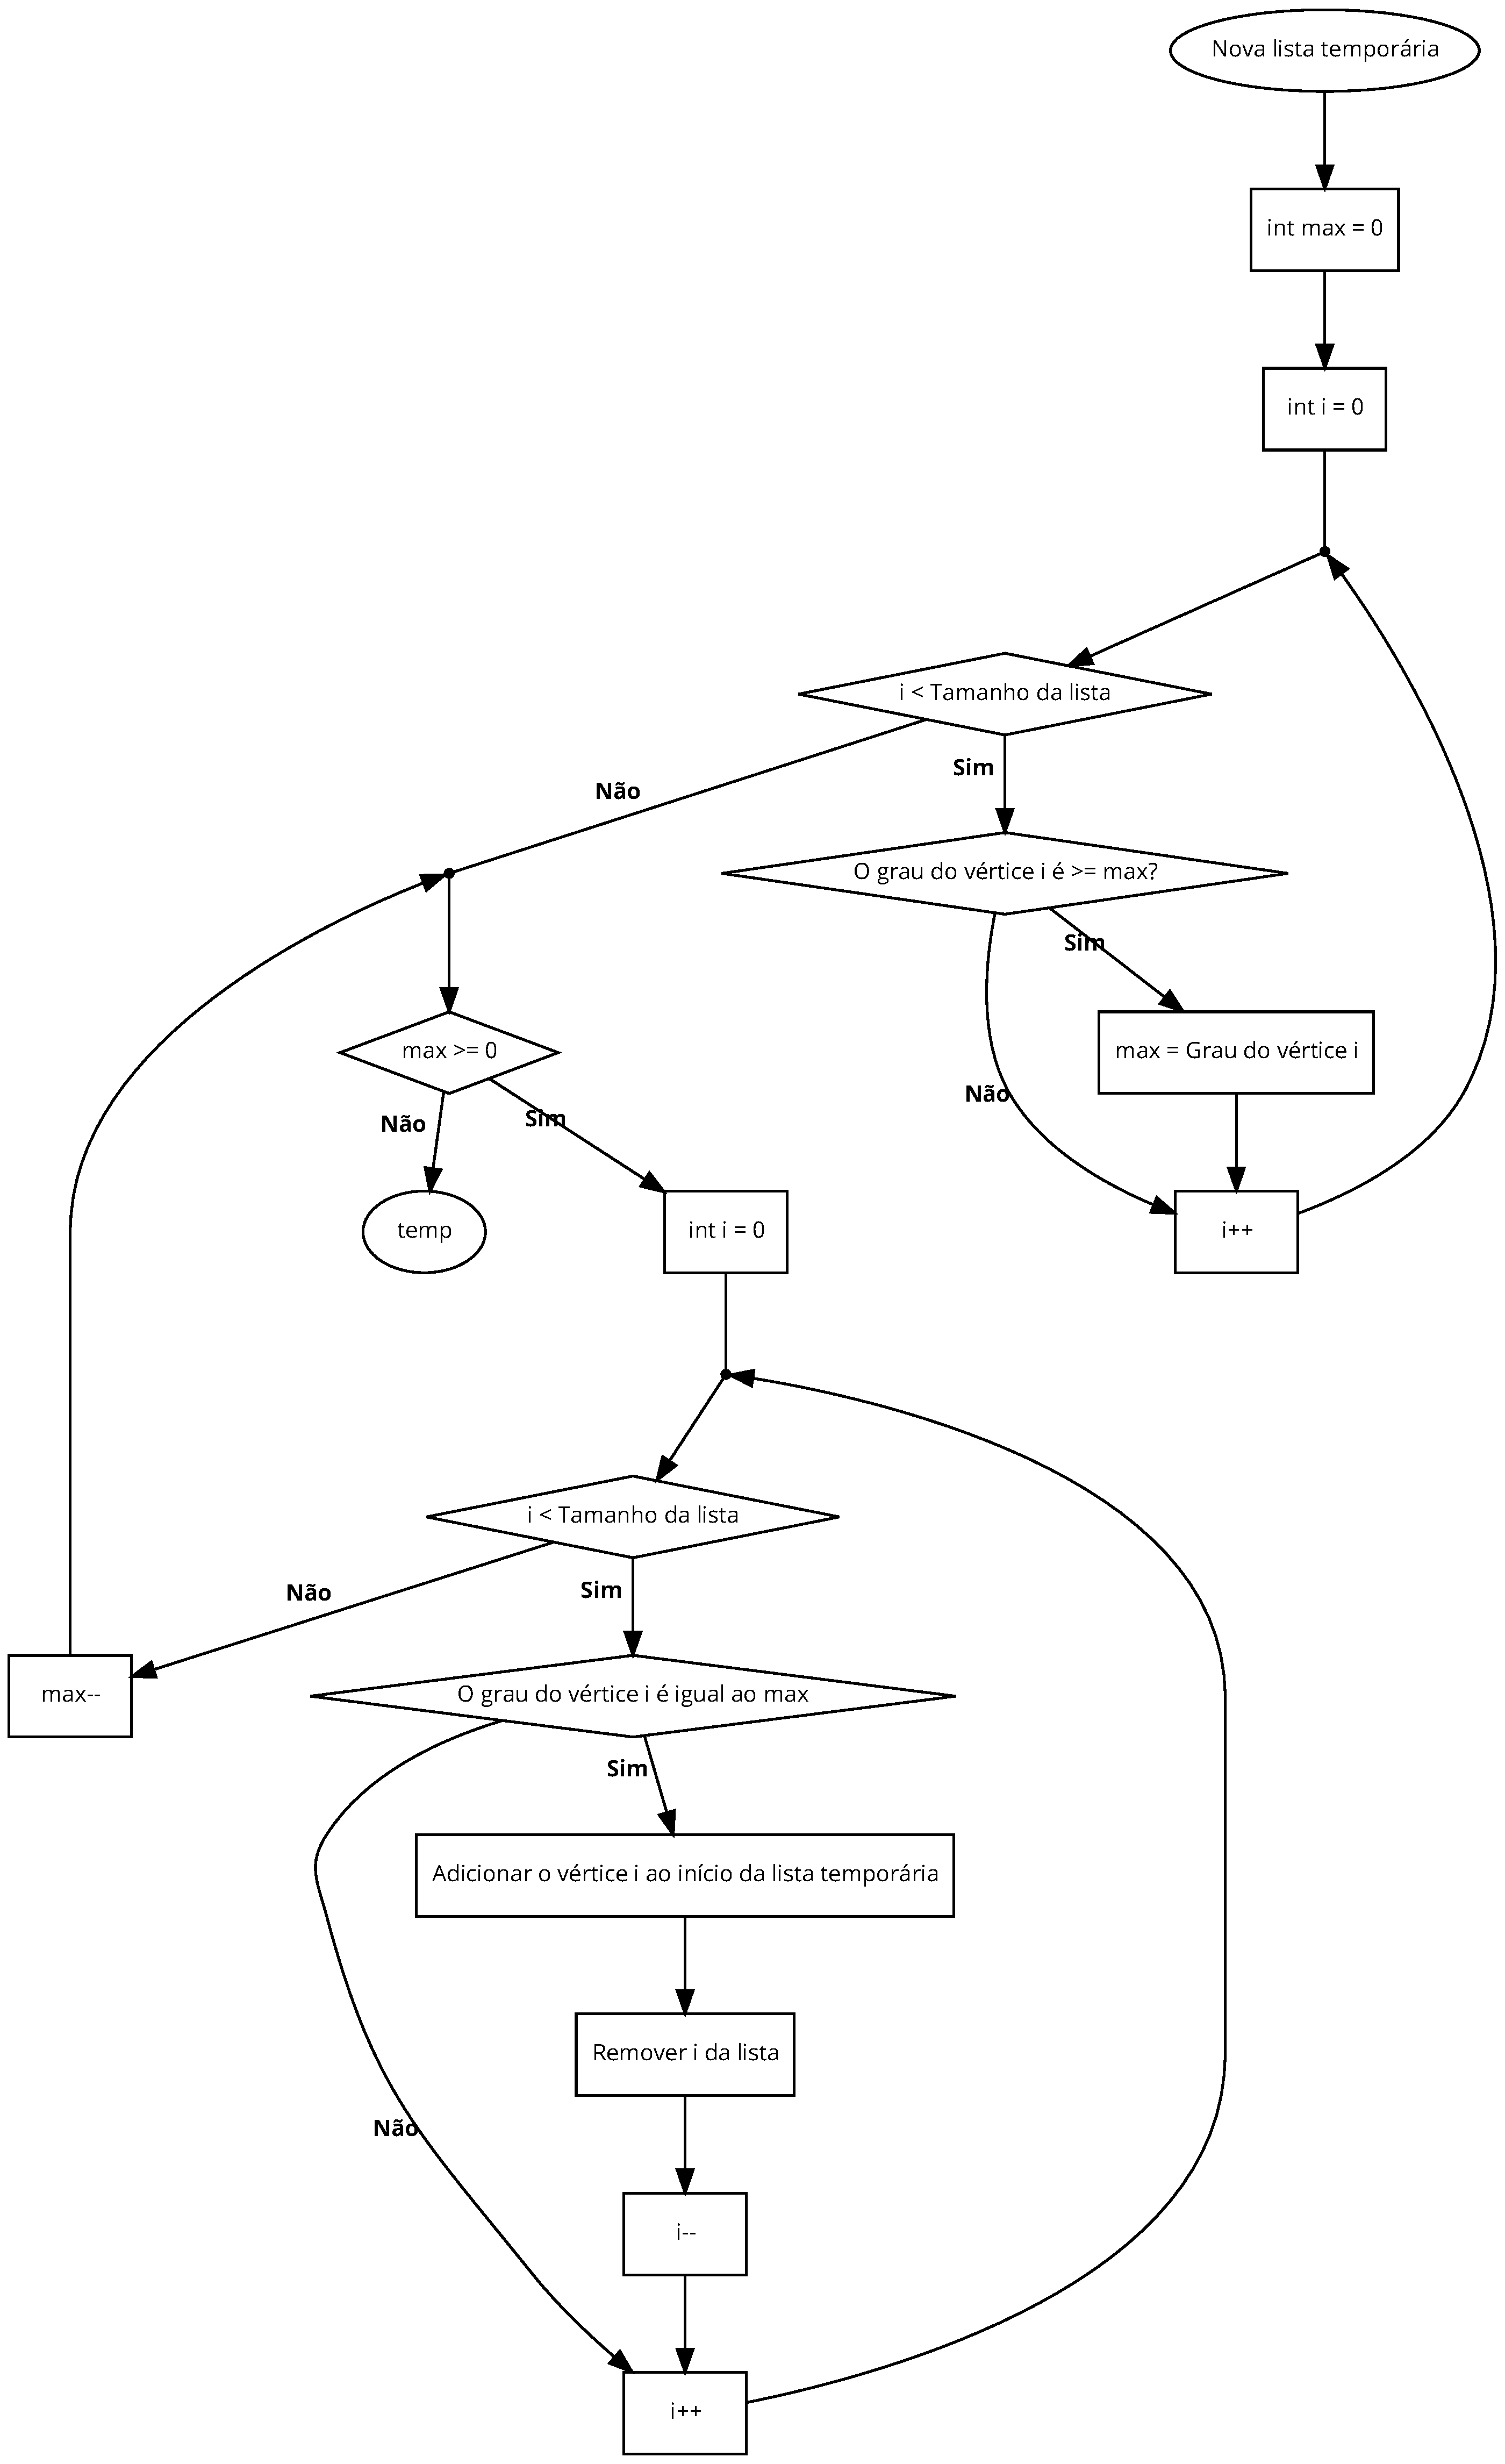
\includegraphics[scale=0.18]{img/ordernarVerticesPorGrau.pdf}
    \caption{Ordenar os vértices por ordem crescente de grau}
    \label{fig:ovpg}
\end{figure}

\begin{lstlisting}
        ArrayList<Vertex> temp = new ArrayList<Vertex>();
        int max = 0;
        for (int i = 0; i < vertexList.size(); i++)
            if (vertexList.get(i).getDegree() >= max) 
                max = vertexList.get(i).getDegree();
        while (max >= 0) {
            for (int i = 0; i < vertexList.size(); i++) {
                if (vertexList.get(i).getDegree() == max){
                    temp.add(0, vertexList.get(i));
                    vertexList.remove(i);
                    i--;
                }
            }       
            max--;
        }
        return temp;
\end{lstlisting}

O método \textit{sortVertexByDegree ()} organiza a lista de vértices deste grafo pela ordem do grau de cada vértice.

\begin{lstlisting}
        vertexList = getVertexByDegree();
\end{lstlisting}

O método \textit{setDefaultColorVertexes ()} define a cor de cada vértice como 0 (cor inicial).

\begin{lstlisting}
        for (int i = 0; i < vertexList.size(); i++)
            vertexList.get(i).setColor(0);
\end{lstlisting}

\section{Vértice (\textit{Vertex.java})}\label{vertex}

Esta estrutura representa um vértice, identificado por um \textit{id}, \textit{color}, \textit{order}, por um atributo que define se o vértice foi ou não visitado (\textit{visited}), por uma lista de vértices sucessores (\textit{sucessorList}) e uma lista de predecessores (\textit{predecessorList}).

\begin{lstlisting}
    private int id, color, order;
    private boolean visited;
    private ArrayList<Integer> successorList, predecessorList;
\end{lstlisting}

O método \textit{getId ()} retorna o \textit{id} do vértice.

\begin{lstlisting}
    return id;
\end{lstlisting}

O método \textit{setColor (int color)} define a cor do vértice com a cor \textit{color}.

\begin{lstlisting}
    this.color = color;
\end{lstlisting}

O método \textit{getColor ()} retorna a cor do vértice.

\begin{lstlisting}
    return color;
\end{lstlisting}

O método \textit{setOrder (int order)} define a ordem do vértice com o número \textit{order}.

\begin{lstlisting}
    this.order = order;
\end{lstlisting}

O método \textit{setVisited ()} define o vértice como visitado.

\begin{lstlisting}
    visited = true;
\end{lstlisting}

O método \textit{isVisited ()} retorna um booleano que indica se o vértice já foi ou não visitado.

\begin{lstlisting}
    return visited;
\end{lstlisting}

O método \textit{setNeighbors (int k, int ps)} define este vértice como vizinho do vértice identificado por k. Se ps for $1$ então o vértice k é sucessor, caso contrário k é predecessor.

\begin{lstlisting}
    if (ps == 1) {
        if (!successorList.contains(k))
            successorList.add(k);
    }
    else if (ps == -1) {
        if (!predecessorList.contains(k))
            predecessorList.add(k);
    }
\end{lstlisting}

O método \textit{isNeighbor (int k)} retorna um valor booleano que indica se o vértice é vizinho do vértice k.

\begin{lstlisting}
    return (successorList.contains(k) || predecessorList.contains(k));
\end{lstlisting}

O método \textit{getNeighborList ()} retorna a lista de sucessores e predecessores do vértice.

\begin{lstlisting}
    Set<Integer> set = new HashSet<Integer>();
    set.addAll(successorList);
    set.addAll(predecessorList);
    return new ArrayList<Integer>(set);
\end{lstlisting}

O método \textit{getSucessorList ()} retorna a lista de sucessores do vértice.

\begin{lstlisting}
    return sucessorList;
\end{lstlisting}

O método \textit{getPredecessorList ()} retorna a lista de predecessores do vértice.

\begin{lstlisting}
    return predecessorList;
\end{lstlisting}

O método \textit{getDegree ()} retorna o grau do vértice. Este é igual ao número de vizinhos do vértice.

\begin{lstlisting}
    return getNeighborList().size();
\end{lstlisting}

\section{Coloração dos vértices, versão 1}

Esta implementação recebe um objeto do tipo grafo (\textit{Graph.java}) e contém um conjunto de métodos que permite desenvolver um algoritmo de \textit{fácil} leitura.
Quando invocada, esta implementação guarda a lista dos vértices do grafo e define todos os vértices com a cor $0$ (para garantir que o vértice não foi colorido anteriormente com outra cor distinta).

\begin{lstlisting}
    graph.setDefaultColorVertexes();
    vertexList = graph.getVertexList();
\end{lstlisting}

O método \textit{setColorVertex (int id)} define a cor do vértice identificado pelo \textit{id} com a primeira cor disponível (tendo em conta os seus vizinhos), com recurso ao método \textit{getFirstColorAvailable ()}. 
No caso do \textit{id} ser $-1$ significa que o vértice a colorir é o último vértice da lista.
Após obter o vértice correspondente ao \textit{id} obtém a primeira cor disponível (\textit{color}) e atribui ao vértice a cor \textit{color}.

\begin{figure}[H]
    \centering
        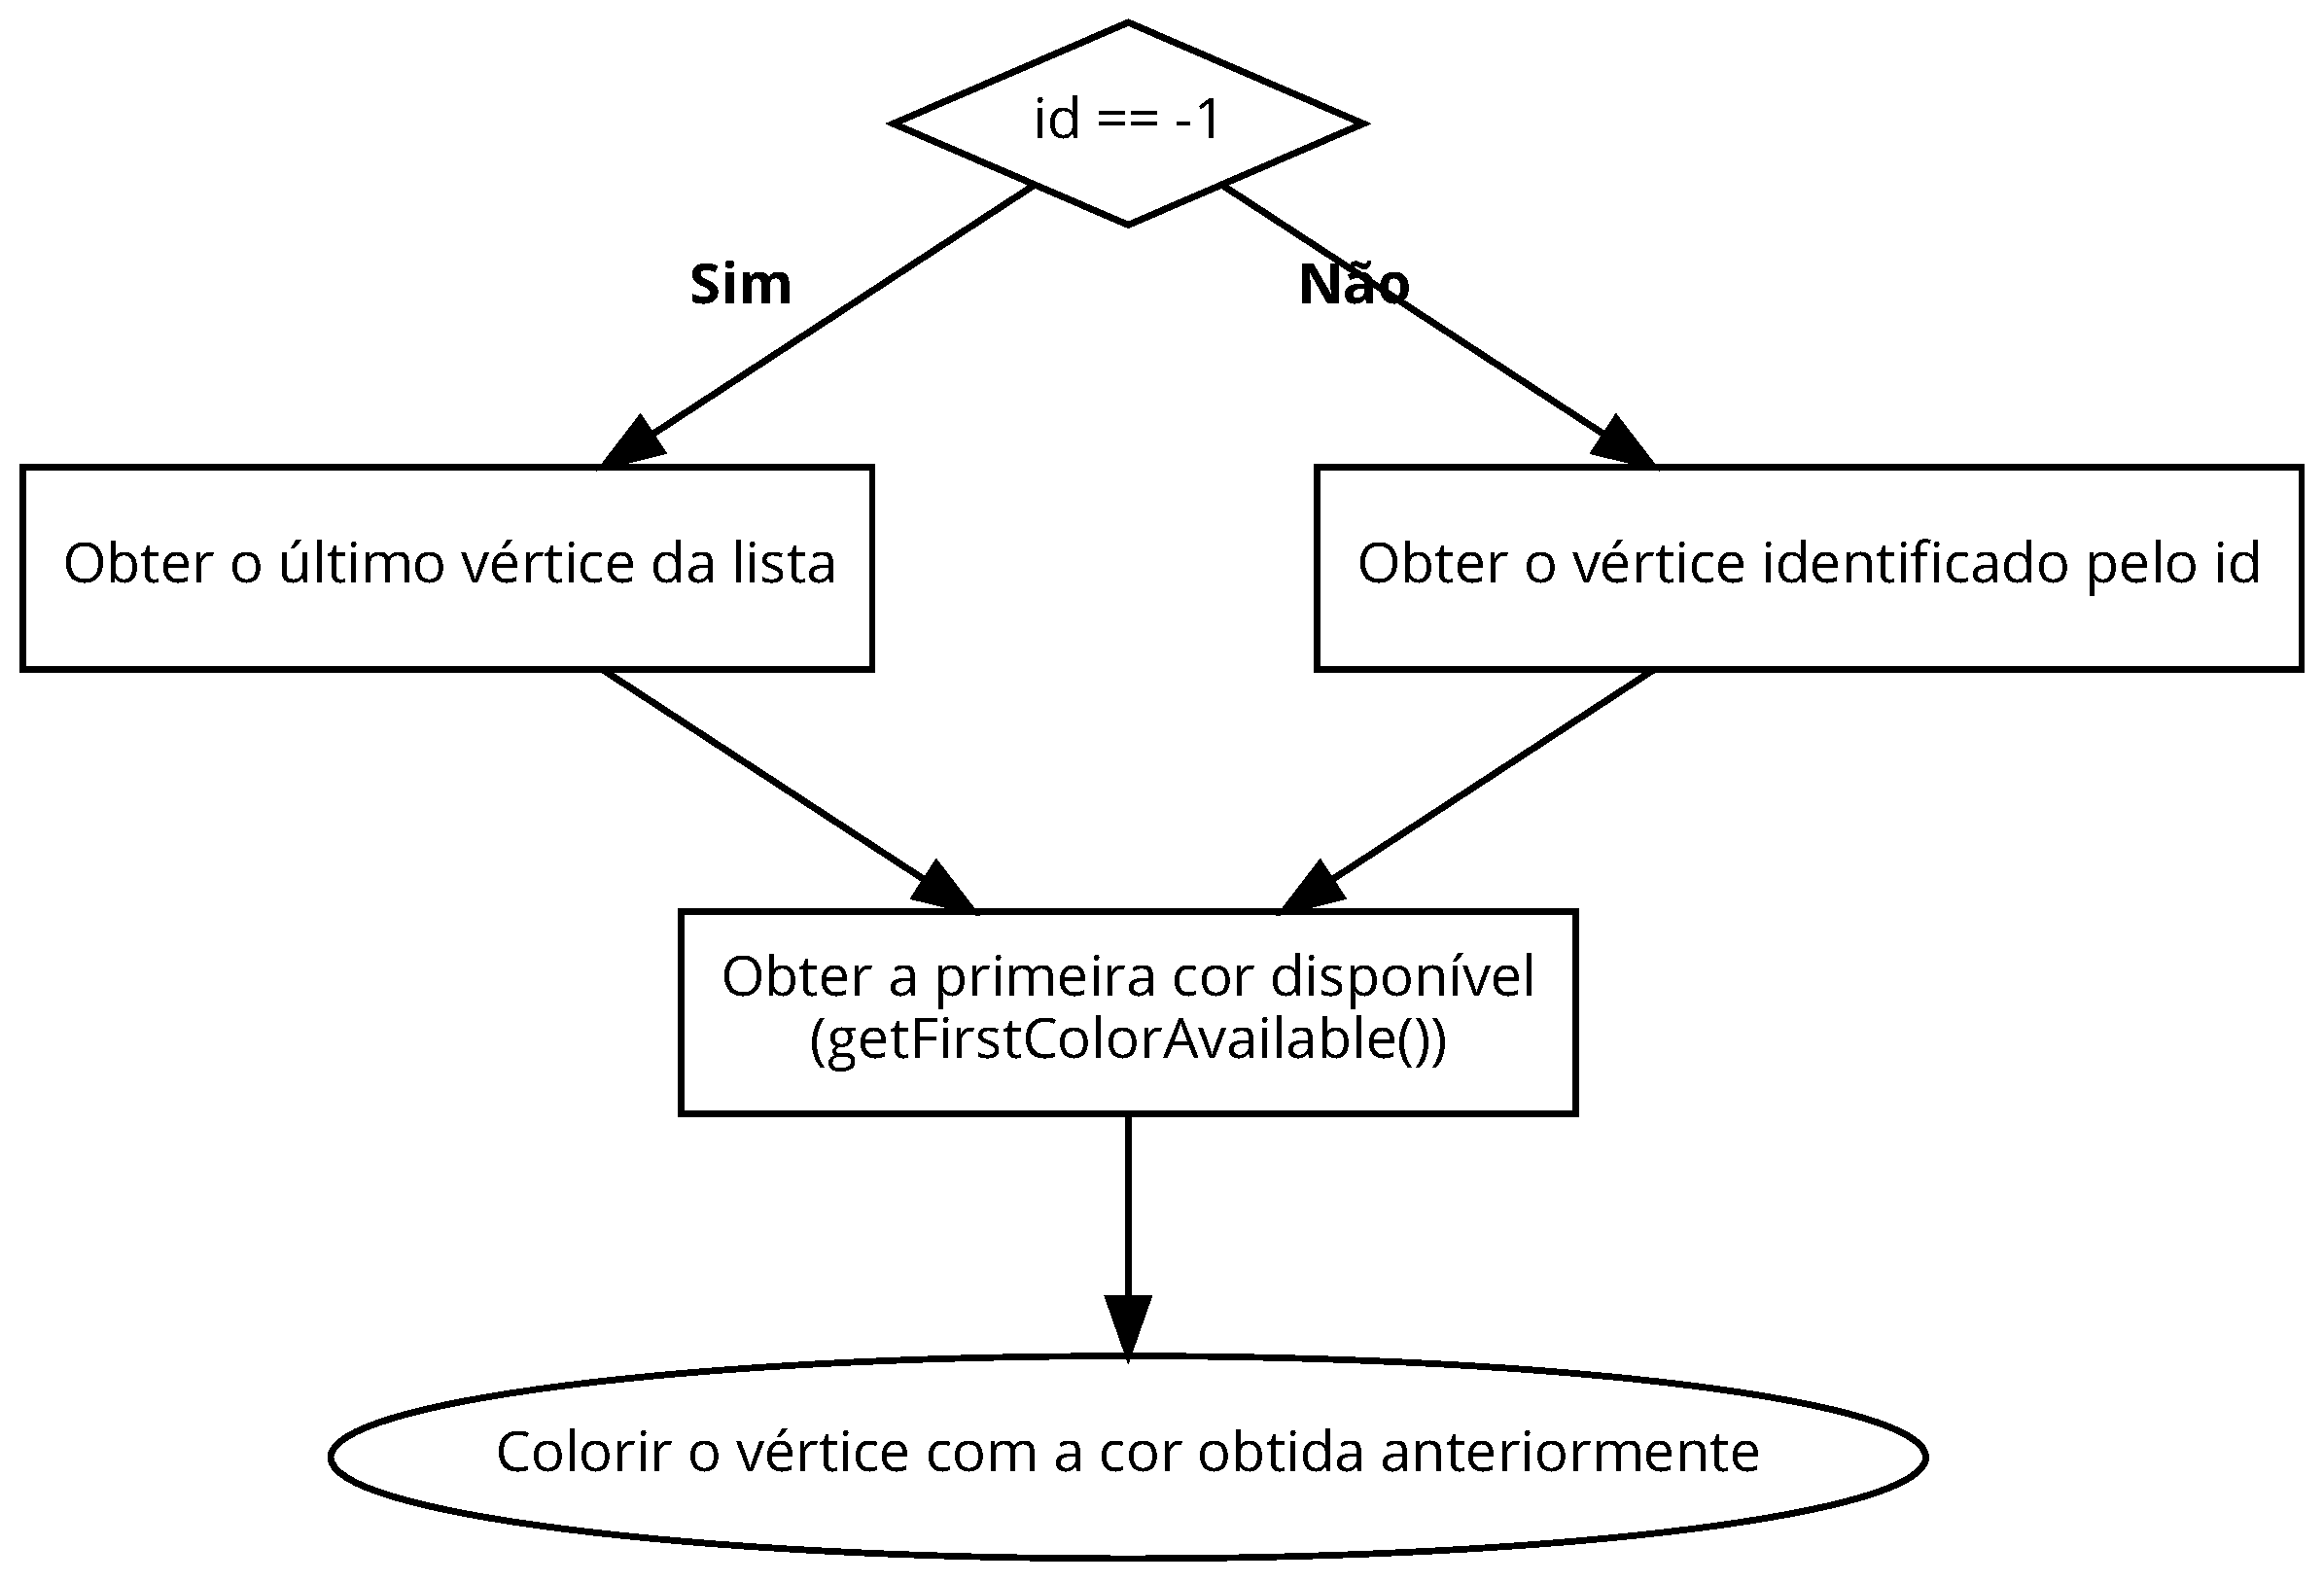
\includegraphics[scale=0.25]{img/setColorVertex.pdf}
    \caption{Definir a cor do vértice}
    \label{fig:scv}
\end{figure}

\begin{lstlisting}
    Vertex vertex;
    if (id == -1)   
        vertex = vertexList.get(vertexList.size()-1);
    else
        vertex = vertexList.get(id);
    int color = getFirstColorAvailable();
    vertex.setColor(color);
\end{lstlisting}

O método \textit{getFirstColorAvailable ()} analisa uma fila de cores e retorna a cor mínima disponível. Esta fila é preenchida no método \textit{saveNeighborColors (int j)}.
Inicialmente começa com a cor mínima k = 1 e verifica se esta cor existe na lista de cores. 
No caso de exisitir então k passa a ser igual a 2 e volta a verificar se 2 existe na lista de cores. Este processo é repetido até encontrar um k que não conste na lista de cores.

\begin{figure}[H]
    \centering
        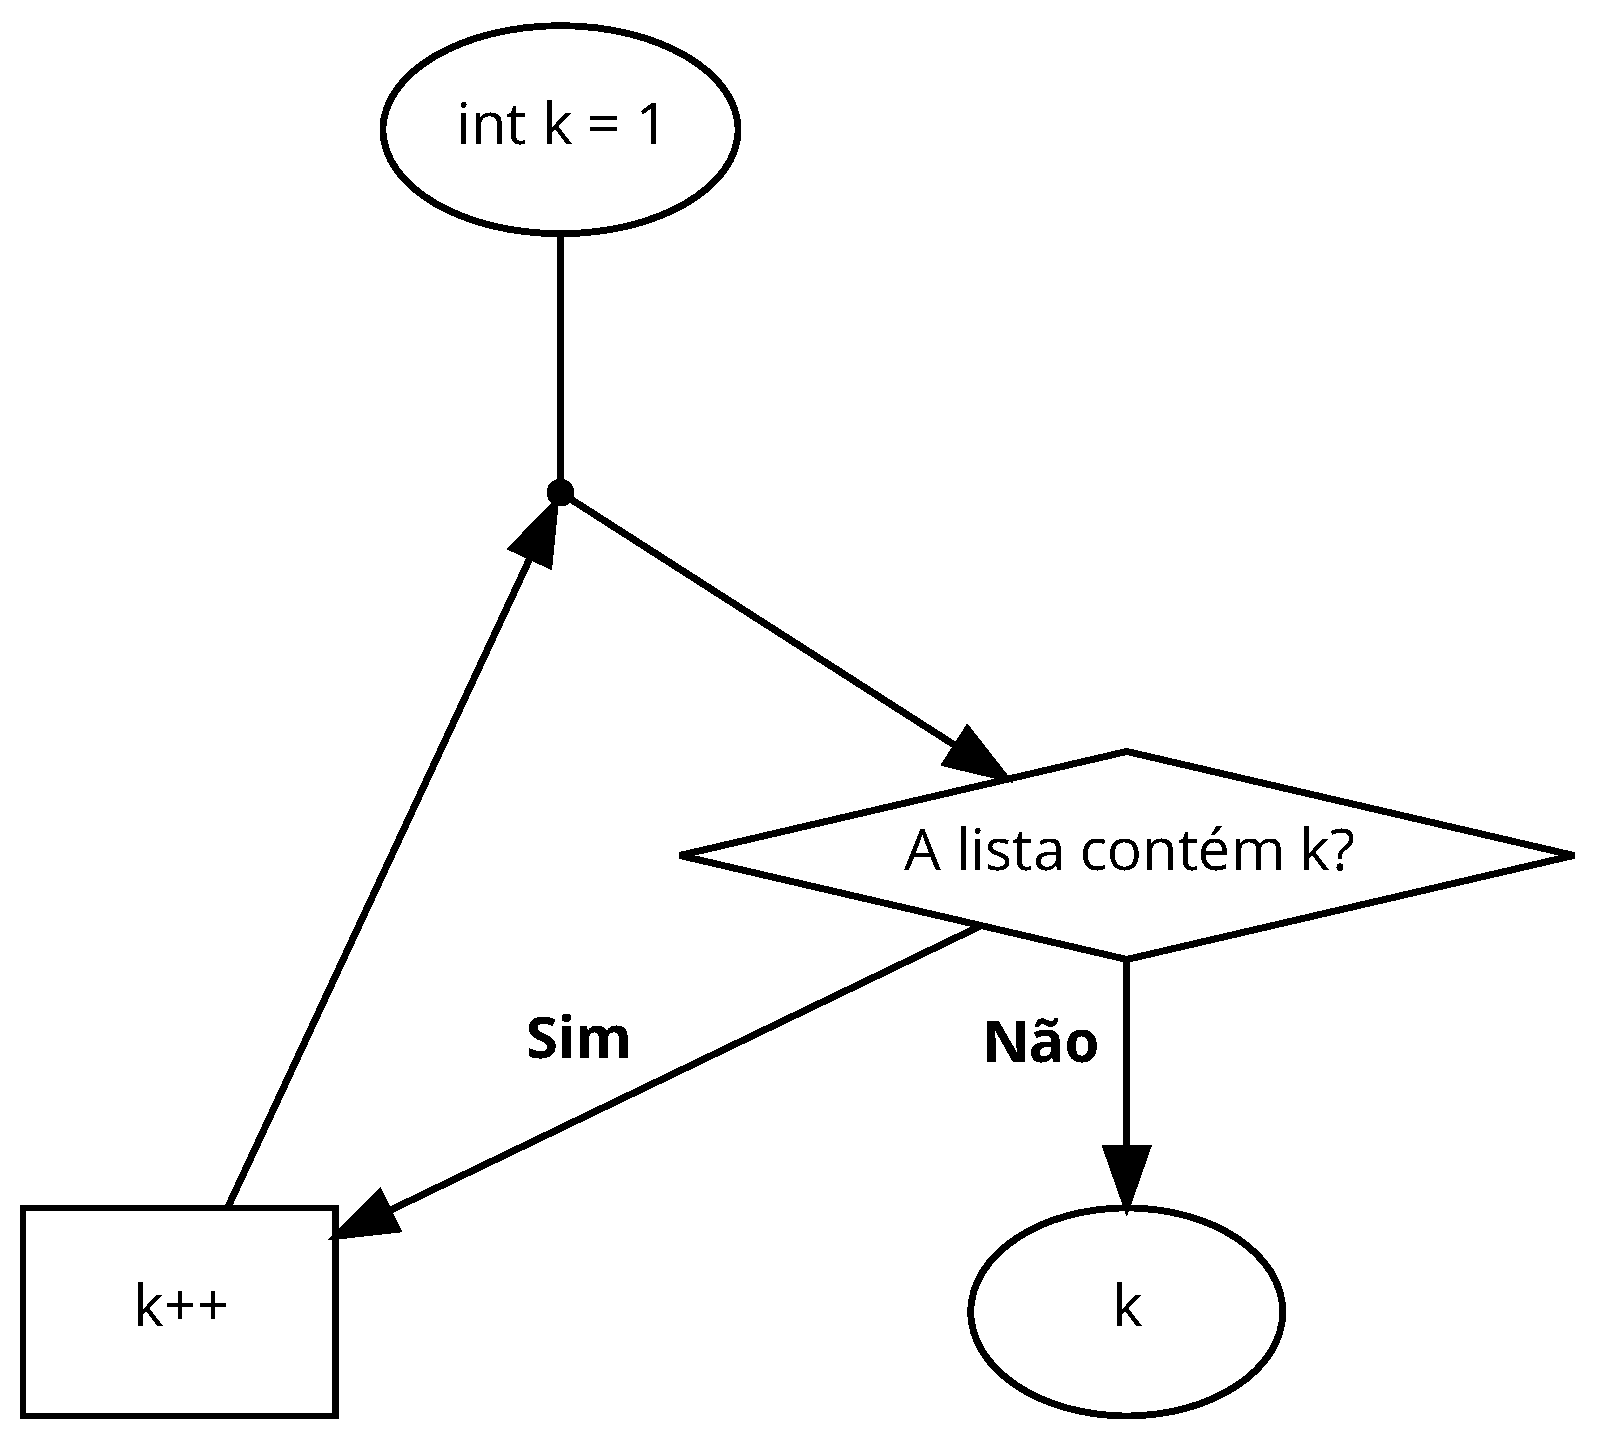
\includegraphics[scale=0.25]{img/getFirstColorAvailable.pdf}
    \caption{Obter a primeira cor disponível}
    \label{fig:gfca}
\end{figure}

\begin{lstlisting}
    int k = 1;
    while(colors.contains(k))
        k++;
    return k;
\end{lstlisting}

O método \textit{saveNeighborColors (int j)} guarda as cores dos vizinhos do vértice identificado por j. 
Nesta implementação, apenas verifica se os vértices anteriores são vizinhos, uma vez que como a ordem pela qual são percorridos os vértices começa no primeiro vértice até ao último, então aquando do vértice j ainda só foram coloridos os vértices anteriores.
Quando encontrar um vértice vizinho, adiciona a cor deste à lista de cores.

\begin{figure}[H]
    \centering
        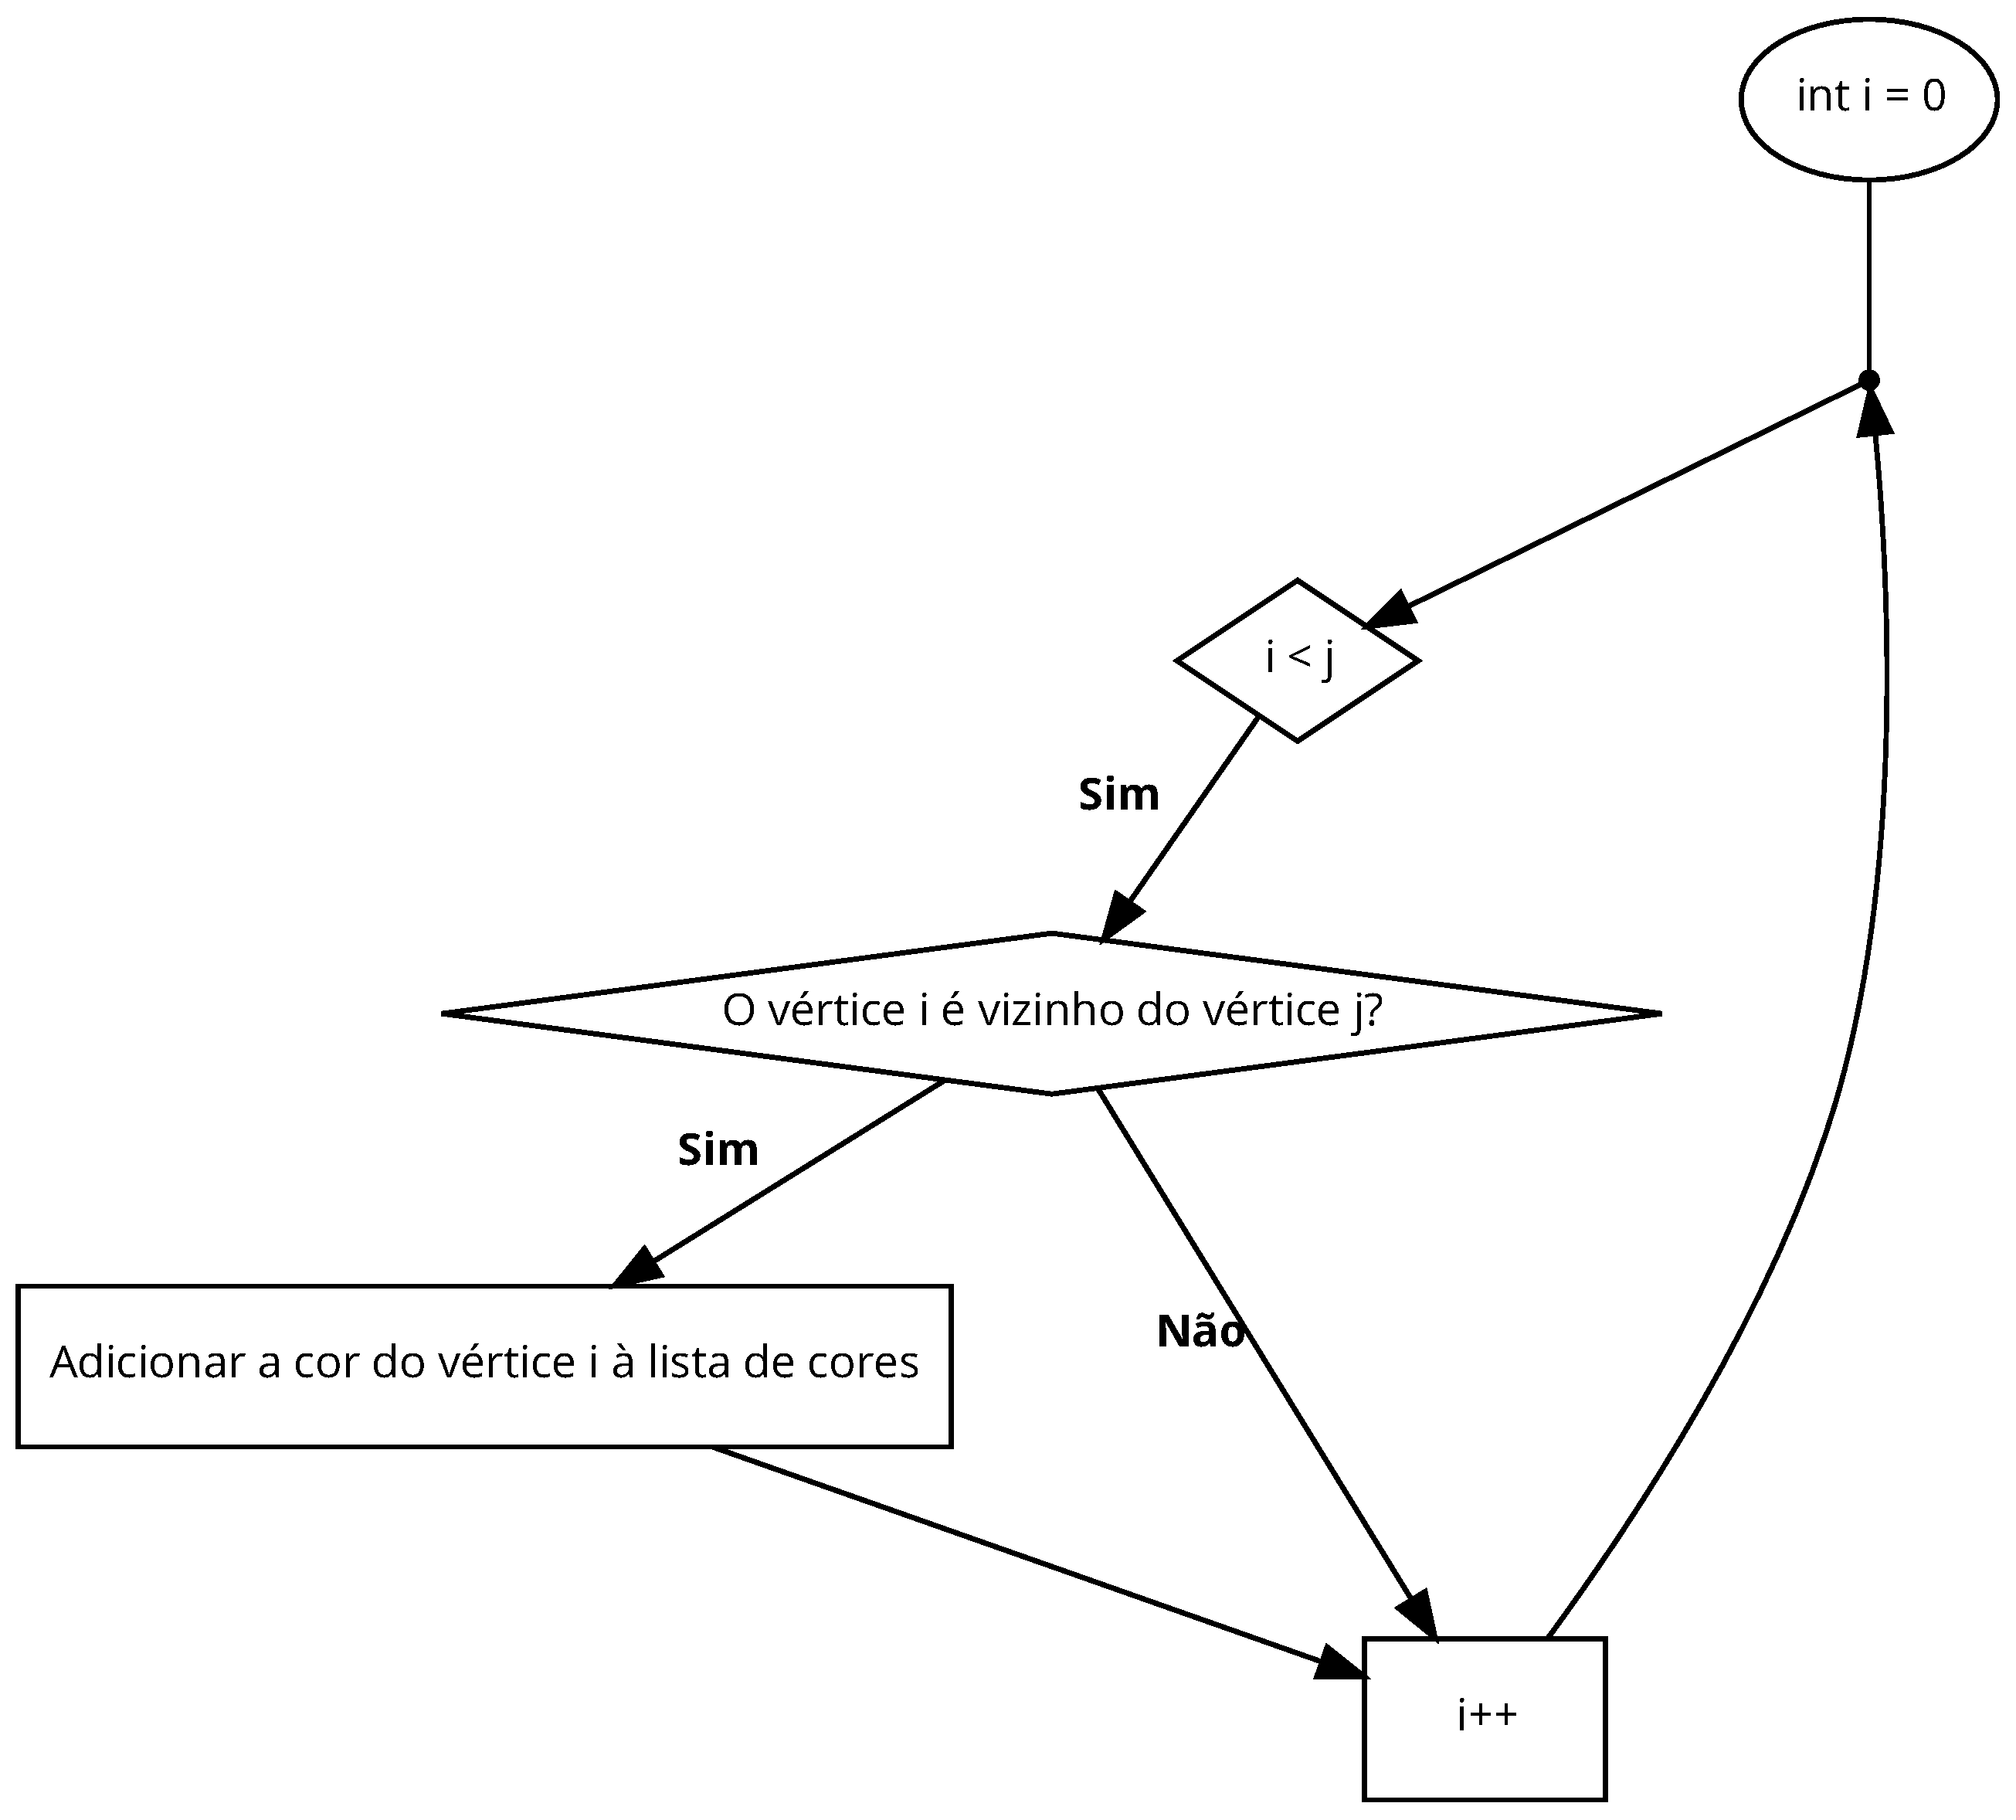
\includegraphics[scale=0.25]{img/saveNeighborColors.pdf}
    \caption{Guardar as cores dos vizinhos}
    \label{fig:snc}
\end{figure}

\begin{lstlisting}
    colors = new LinkedList<Integer>();
    for (int i = 0; i < j; i++)
        if (vertexList.get(j).isNeighbor(vertexList.get(i).getId()))
            colors.add(vertexList.get(i).getColor());
\end{lstlisting}

O método \textit{getVertexList ()} retorna a lista dos vértices do grafo.

\begin{lstlisting}
    return vertexList;
\end{lstlisting}

\subsection*{Algoritmo}

Em suma, seja v1 um objeto do tipo \textit{ColorizeVersion1.java}, definimos a cor do vértice 0 (o primeiro vértice do grafo) com a primeira cor disponível (como é o primeiro vértice, a cor atribuida a este será 1).
Após este processo, percorre-se todos os restantes vértices. A cada um destes, guarda-se a cor dos vértices anteriores que são seus vizinhos e seguidamente é definida a cor do vértice j com a cor mínima disponível (tendo em conta as cores obtidas no processo anterior).
O algoritmo final terá o seguinda aspeto:

\begin{figure}[H]
    \centering
        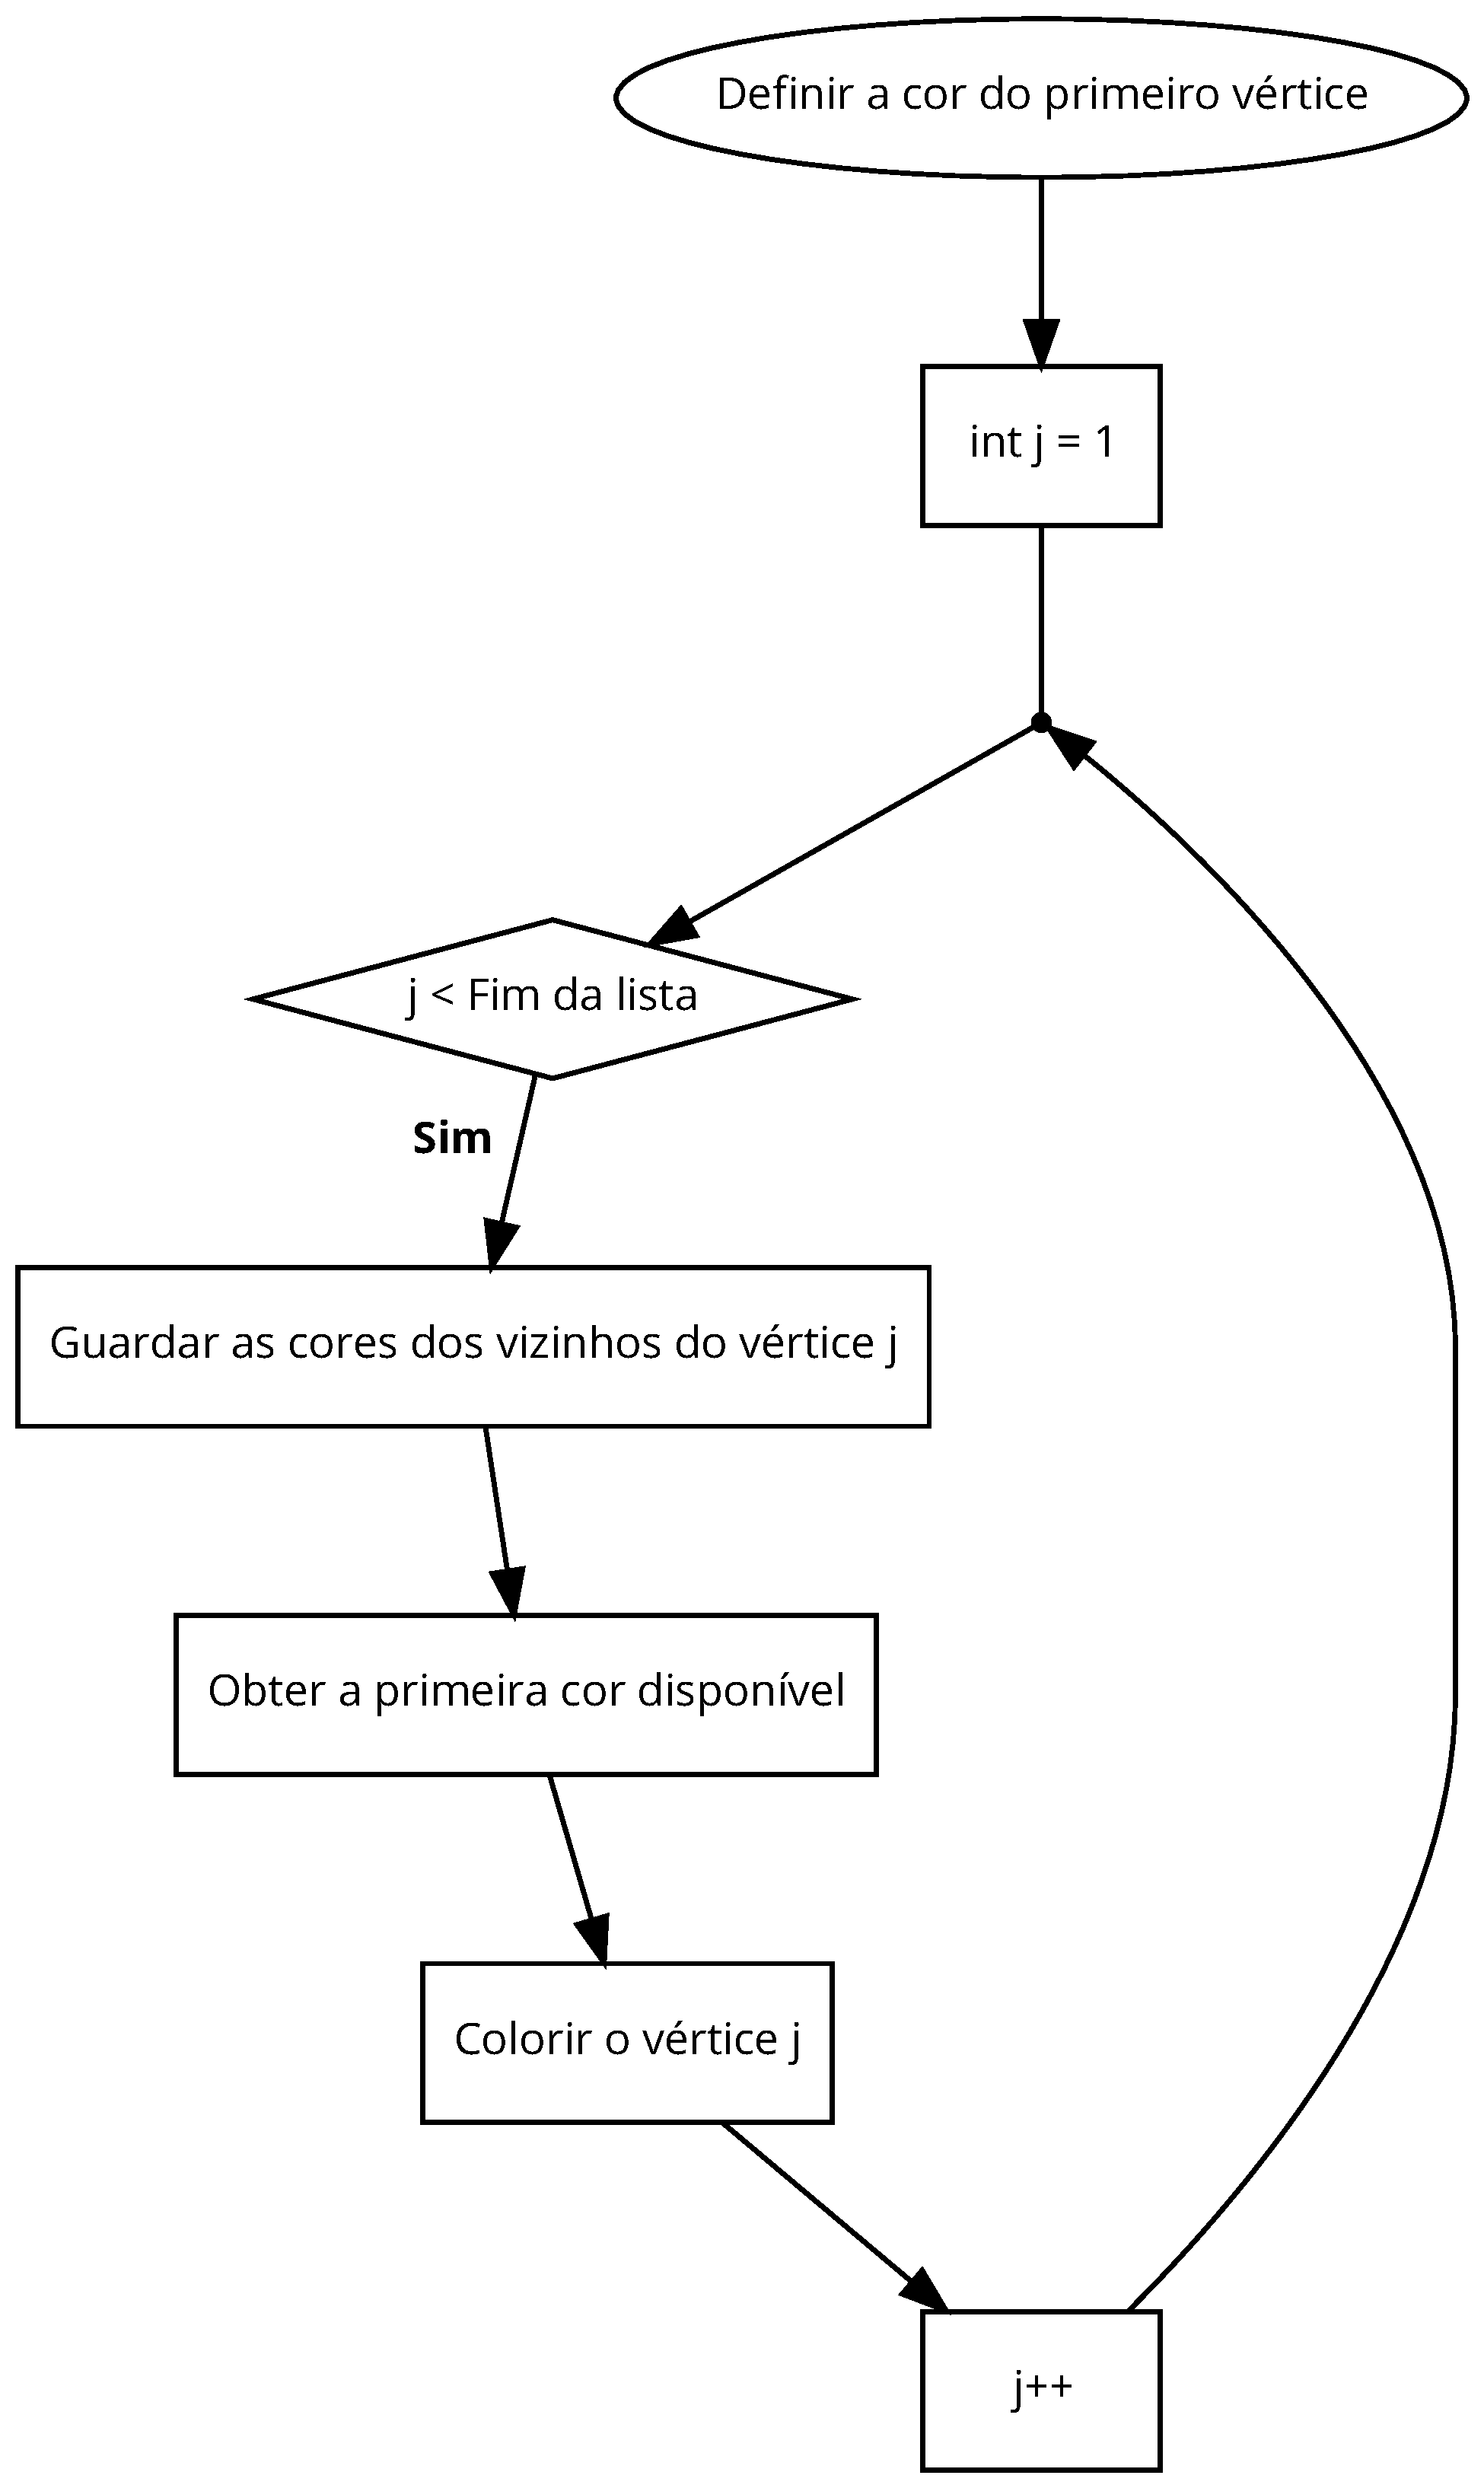
\includegraphics[scale=0.25]{img/colorizeVersion1.pdf}
    \caption{Colorização do grafo, versão 1}
    \label{fig:cV1}
\end{figure}

\begin{lstlisting}
    v1.setColorVertex(0);
    for (int j = 1; j < v1.getVertexList().size(); j++) {
        v1.saveNeighborColors(j);
        v1.setColorVertex(j);
    }
\end{lstlisting}

\section{Coloração dos vértices, versão 2}

Esta implementação, sendo uma extensão da anterior, é em grande parte igual à versão 1. A alteração que implementa é a ordem pela qual verifica os vértices vizinhos, ou seja, apenas verifica os vértices desde o fim até ao vértice j.

\begin{lstlisting}
    colors = new LinkedList<Integer>();
    for (int i = vertexList.size()-1; i > j; i--)
        if (vertexList.get(j).isNeighbor(vertexList.get(i).getId()))
            colors.add(vertexList.get(i).getColor());
\end{lstlisting}

\subsection*{Algoritmo}

Em suma, seja v2 um objeto do tipo \textit{ColorizeVersion2.java}, definimos a cor do último vértice com a primeira cor disponível (como é o primeiro vértice a colorir, a cor atribuida a este será 1).
Após este processo, percorre-se todos os restantes vértices, começando pelo fim (contrariamente à versão anterior). A cada um destes, guarda-se a cor dos seus vizinhos e seguidamente é definida a cor do vértice j com a cor mínima disponível (tendo em conta as cores dos seus vizinhos).
O algoritmo final terá o seguinda aspeto:

\begin{figure}[H]
    \centering
        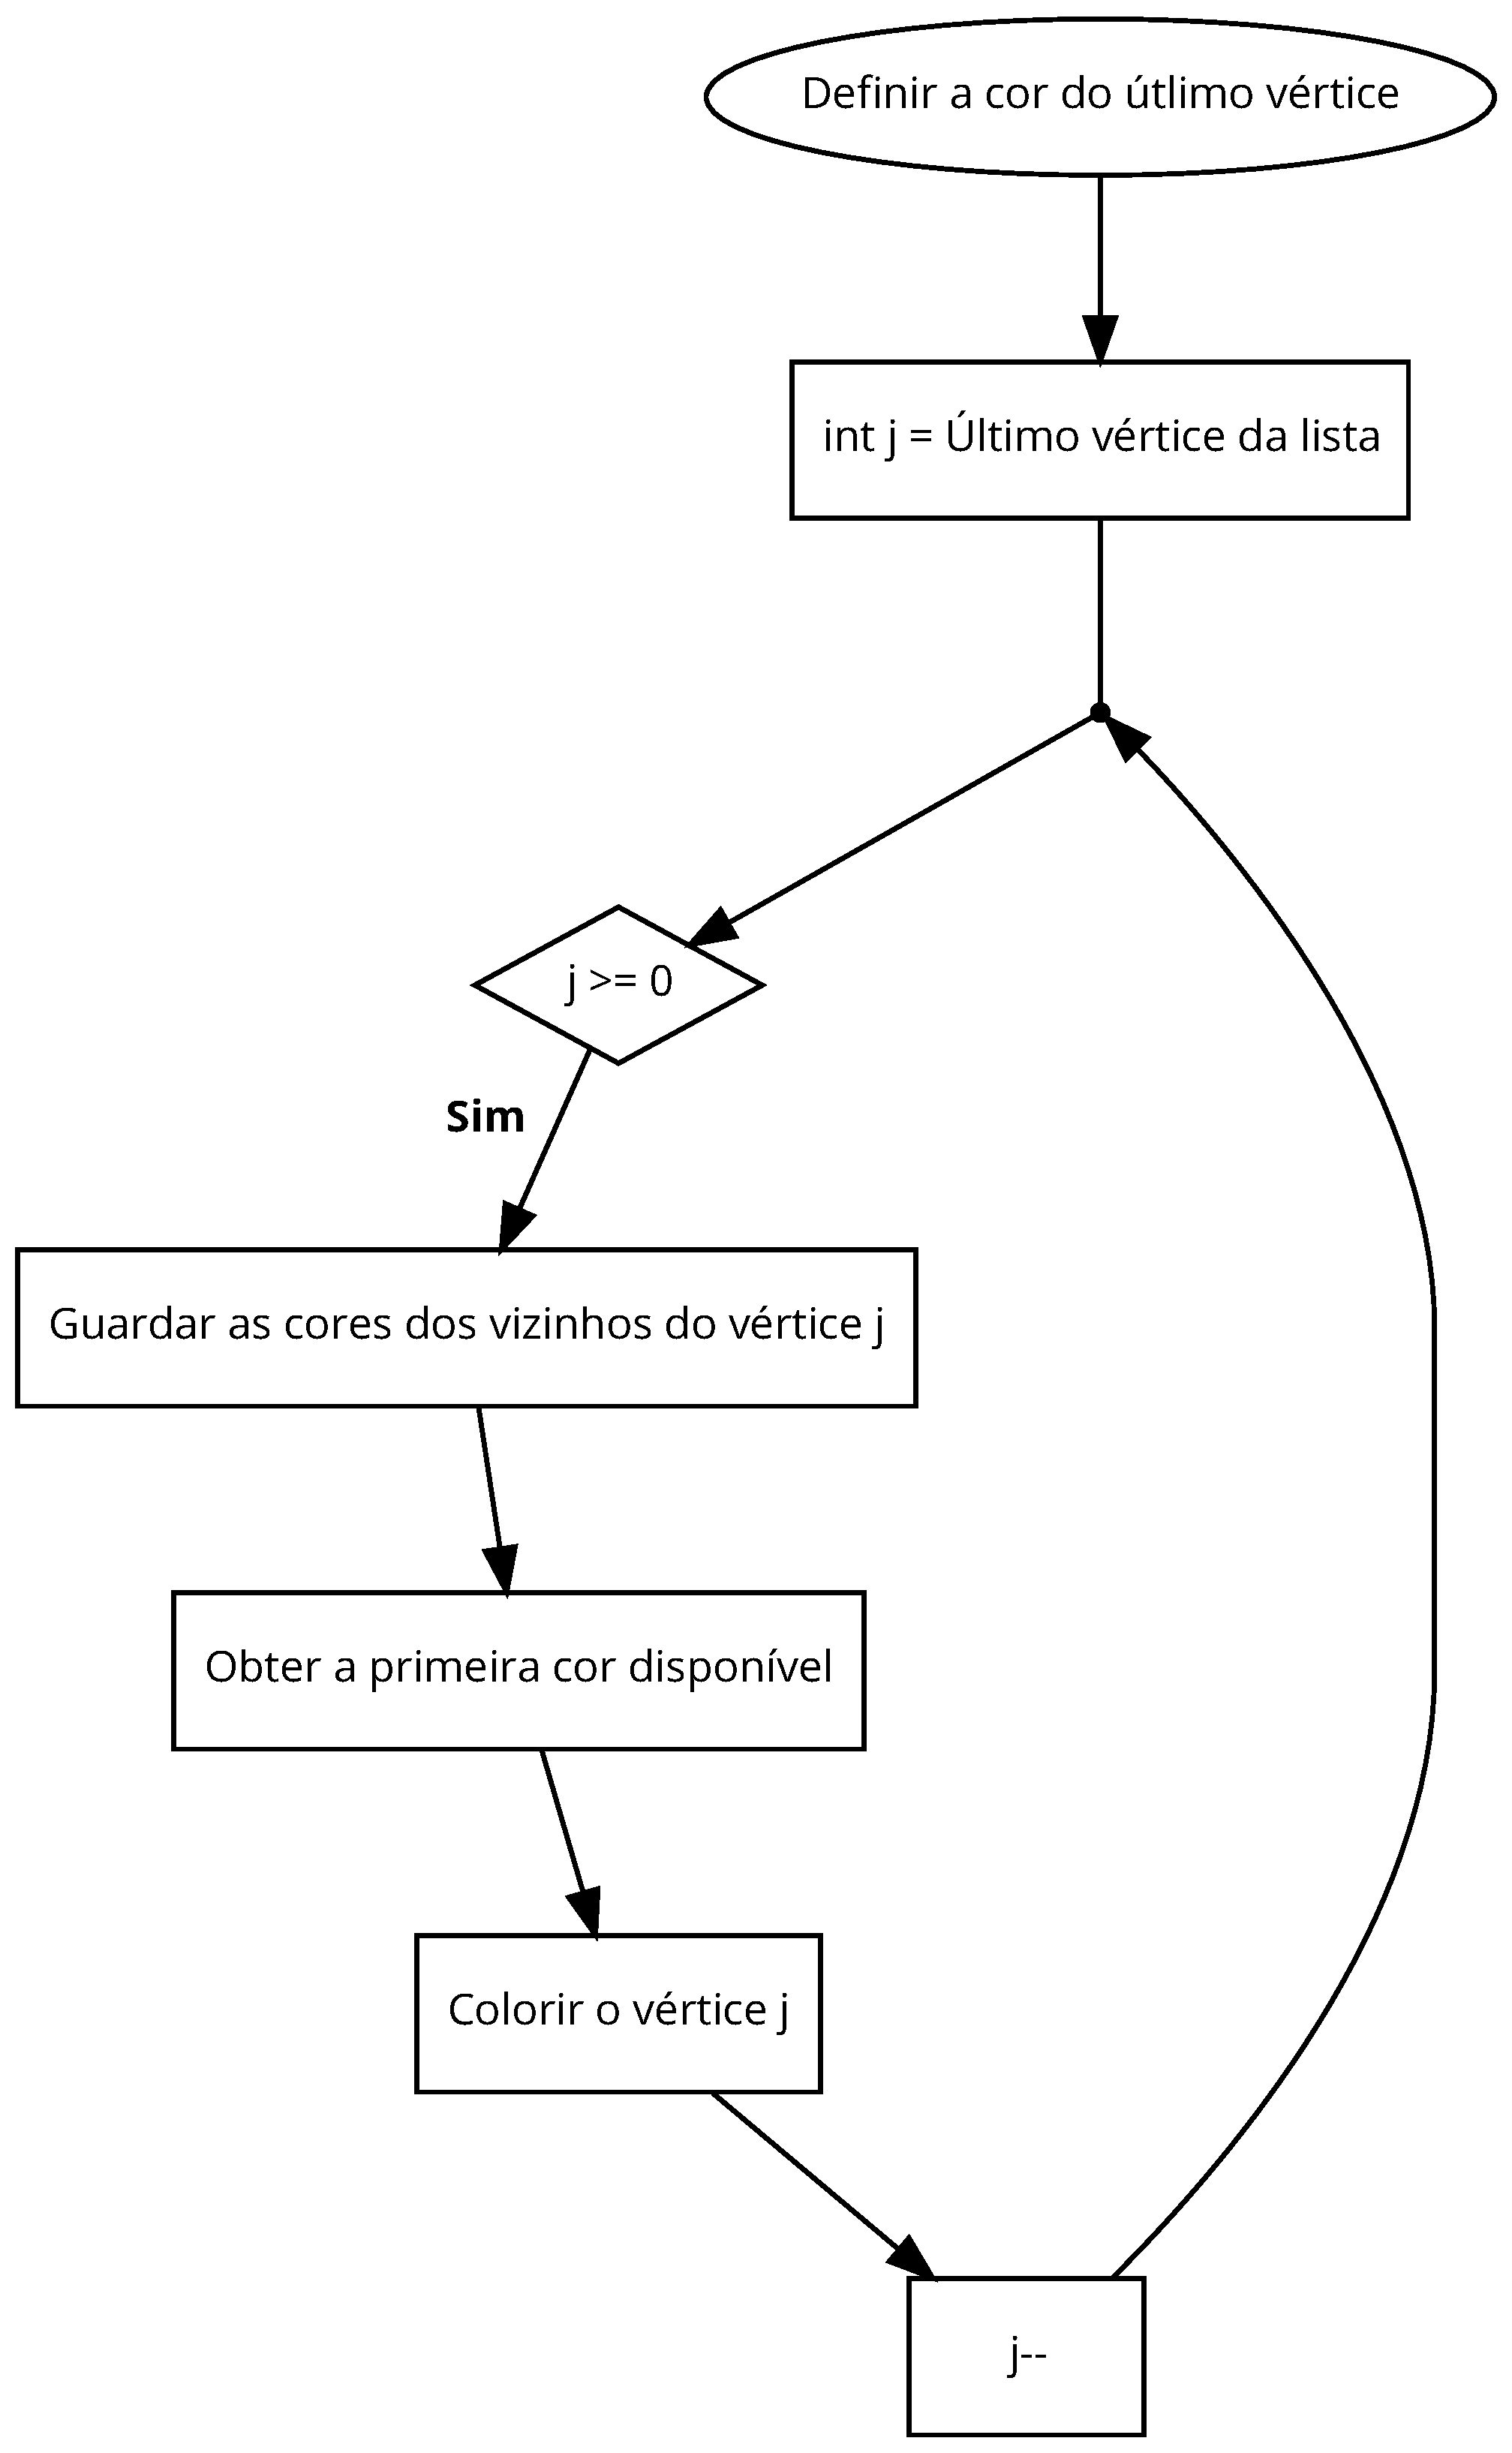
\includegraphics[scale=0.25]{img/colorizeVersion2.pdf}
    \caption{Colorização do grafo, versão 2}
    \label{fig:cV2}
\end{figure}

\begin{lstlisting}
    v2.setColorVertex(-1);
    for (int j = v2.getVertexList().size()-2; j >= 0; j--) {
        v2.saveNeighborColors(j);
        v2.setColorVertex(j);
    }
\end{lstlisting}

\section{Coloração dos vértices, versão 3}

Esta implementação, quando invocada, tem o mesmo comportamento da versão 1 e 2, contudo organiza os vértices pela ordem do seu grau. Uma outra diferença nesta implementação é que ao invês de usar uma lista de cores usa um dicionário em que a chave é o código da cor e o valor é 1 (0 no caso da cor não fazer parte da coloração dos vértices vizinhos de um determinado vértice, e neste caso não é adicionado ao dicionário de cores, 1 no caso de algum vizinho ter a cor identificada pelo código da cor).

\begin{lstlisting}
    colors = new Hashtable<Integer, Integer>();
    vertexByDegree = graph.getVertexByDegree();
\end{lstlisting}

No método \textit{setColorVertex (int id)}, ao invés de se obter os vértices a partir da lista de vértices, o algoritmo recorre à lista dos vértices ordenados por grau. O restante código é igual ao implementado nas versões anteriores.

\begin{lstlisting}
    Vertex vertex;
    if (id == -1)   
        vertex = vertexList.get(vertexByDegree.get(vertexByDegree.size()-1).getId());
    else
        vertex = vertexList.get(vertexByDegree.get(id).getId());
    int color = getFirstColorAvailable();
    vertex.setColor(color);
\end{lstlisting}

O método \textit{saveNeighborColors (int j)} tira proveito do facto de cada vértice ter associado uma lista de vértices vizinhos. Isto permite que o algoritmo não tenha de percorrer todos os vértices do grafo e verificar se algum é vizinho do vértice j e nesse caso adicionar a sua cor à tabela de cores. Neste caso, o algoritmo percorre apenas os vértices que fazem parte da lista de vizinhos do vértice j e adiciona a sua cor à tabela de cores.
Contrariamente a uma lista, a tabela (sendo ela um dicionário) caso contenha a cor que está a adicionar simplesmente atualiza o seu valor (que neste caso fica exatamente igual). Por exemplo, considera-se uma tabela de cores que já contem a cor 2 e 5. Então os valores associados a 2 e 5 é 1 (como foi explicado em cima). Quando se adiciona novamente a cor 2 ou a cor 5, ao invés de criar uma nova entrada nesta tabela de cores, simplesmente verifica se ela já existe antes de criar.

\begin{figure}[H]
    \centering
        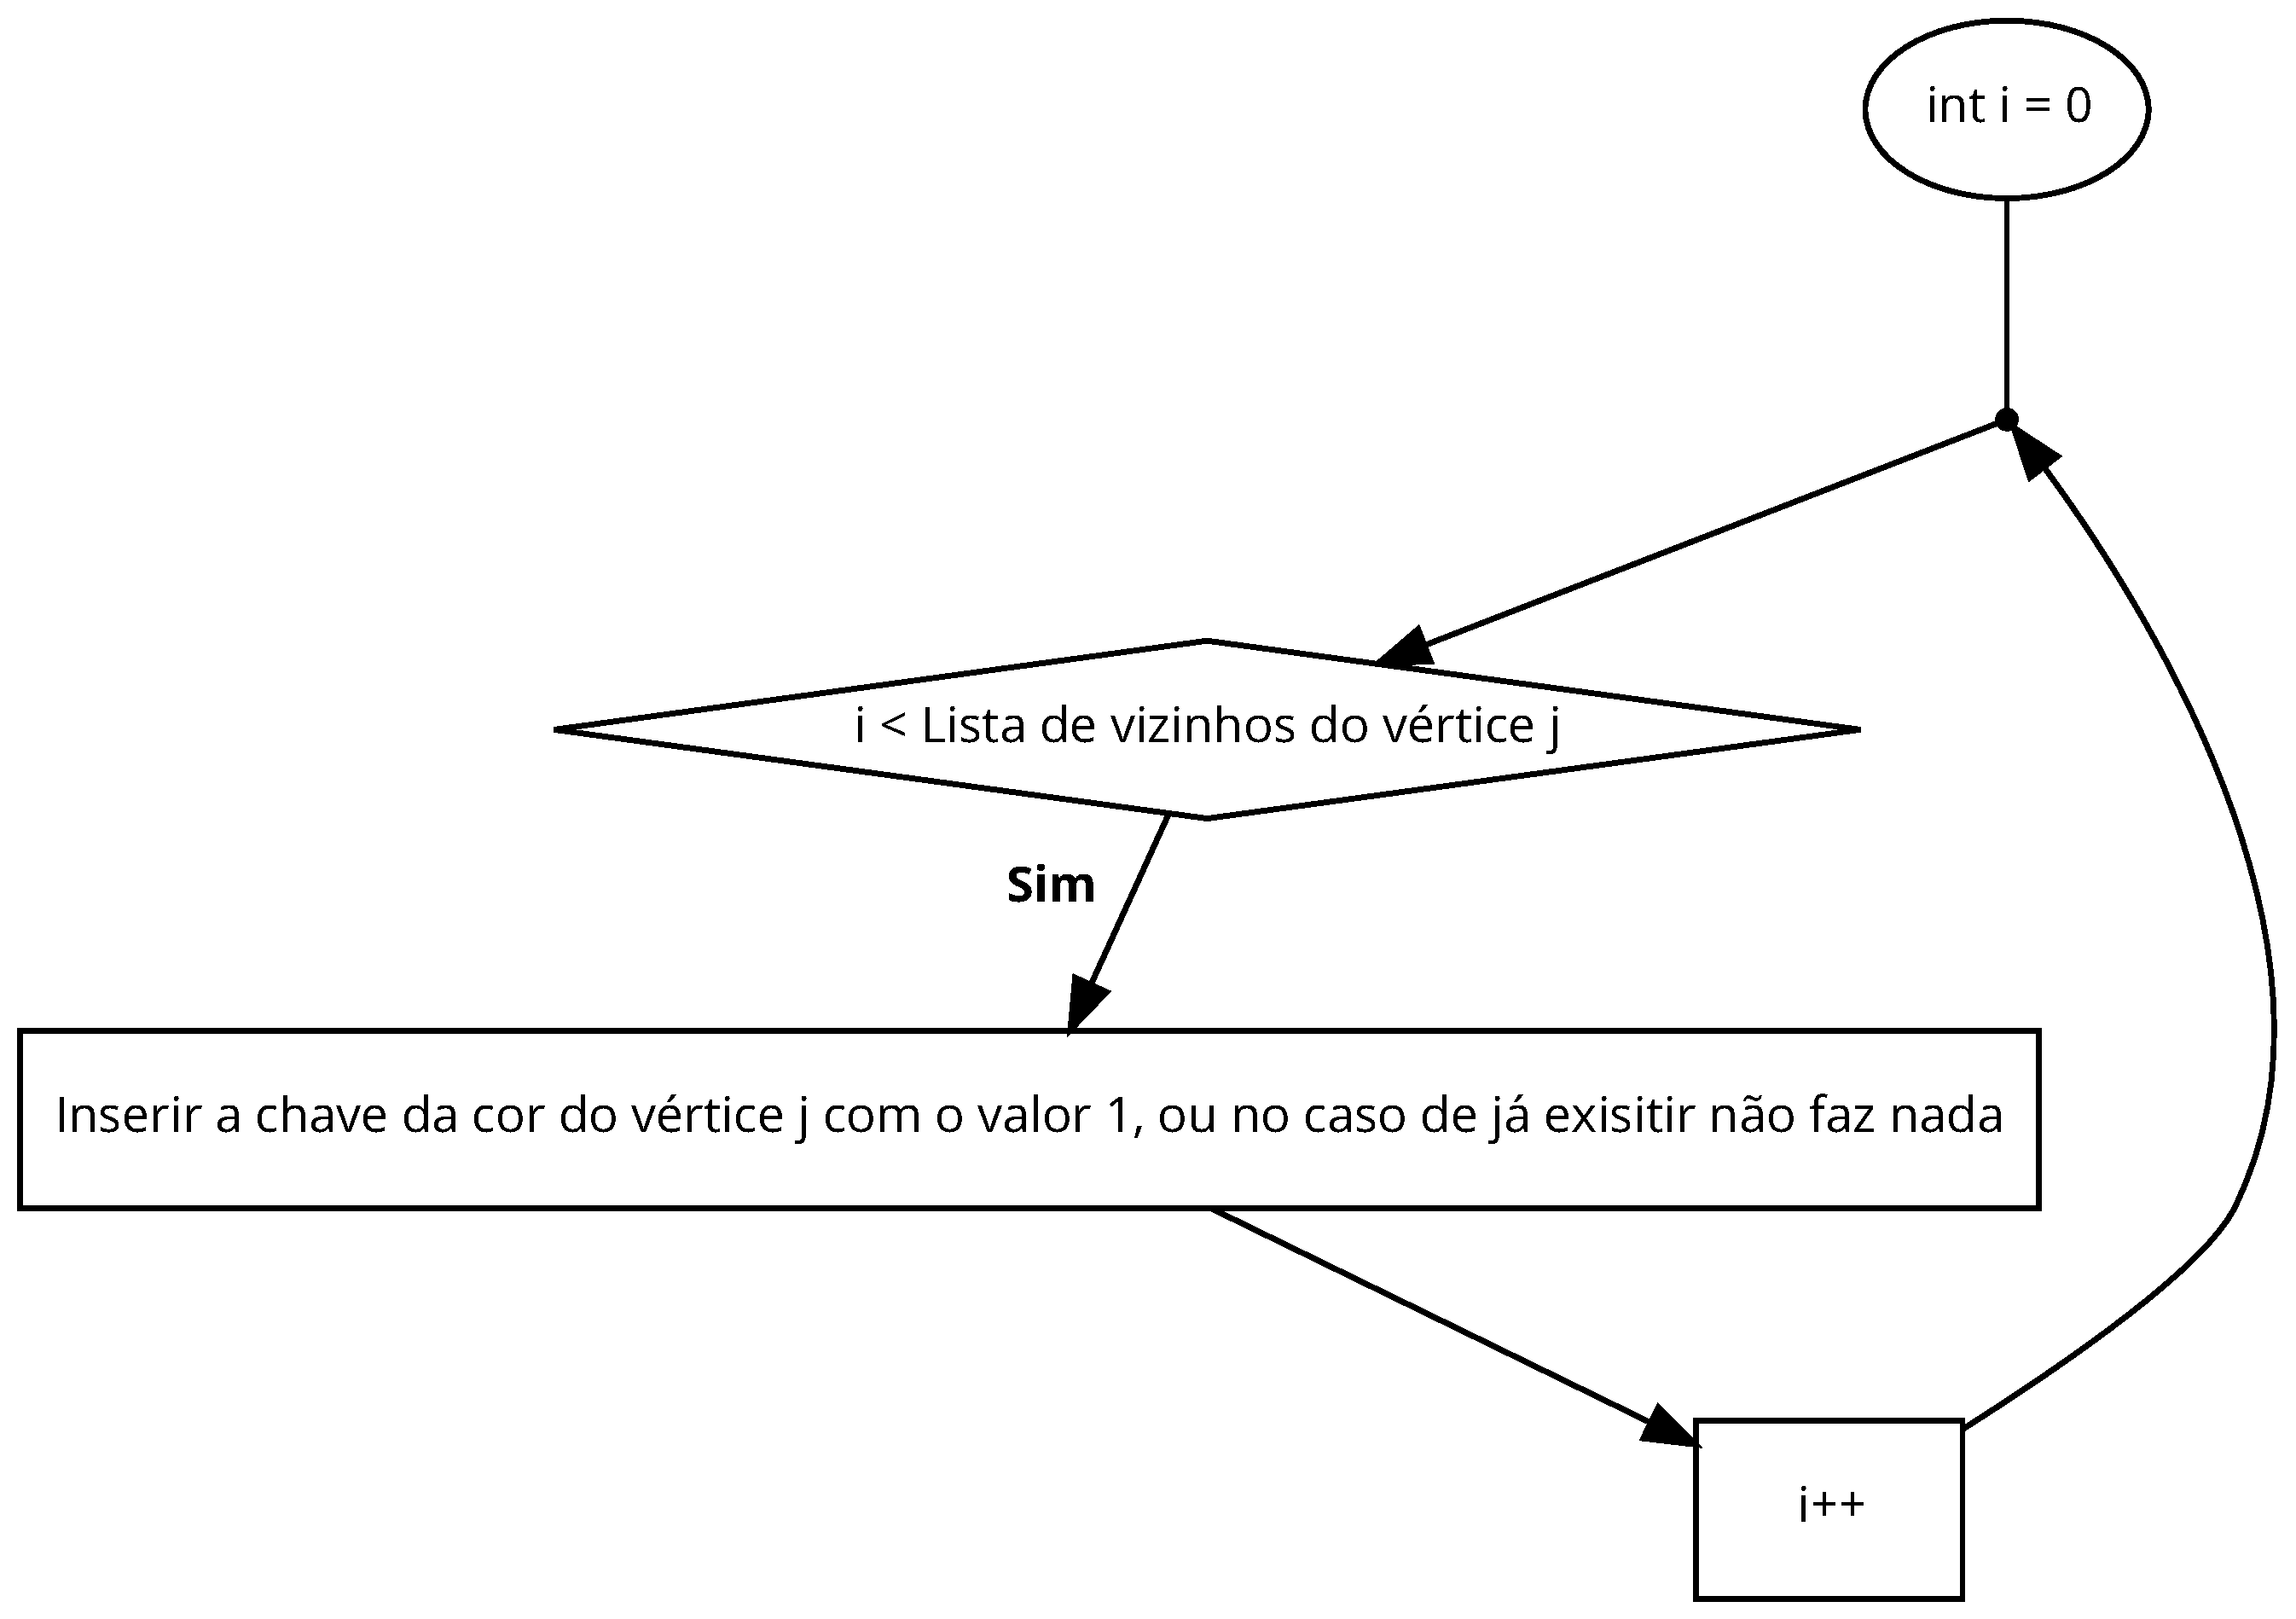
\includegraphics[scale=0.25]{img/saveNeighborColorsV3.pdf}
    \caption{Guardar as cores dos vizinhos, versão 3}
    \label{fig:sncV3}
\end{figure}

\begin{lstlisting}
    colors = new Hashtable<Integer, Integer>();   
    for (int i = 0; i < vertexList.get(vertexByDegree.get(j).getId()).getNeighborList().size(); i++)
        colors.put(vertexList.get(vertexList.get(vertexByDegree.get(j).getId()).getNeighborList().get(i)).getColor(), 1);
\end{lstlisting}

Comparando \ref{fig:snc} com \ref{fig:sncV3} vemos que existe alguma simplificação do processo.

\subsection*{Algoritmo}

Em suma, a implementação deste algoritmo segue a mesma lógica da versão 2, pois uma vez que os vértices estão ordenados por ordem crescente de grau, então começa a percorrer do fim para o início, por forma a atribuir primeiramente as cores aos vértices com maior grau.
Seja v3 um objeto do tipo \textit{ColorizeVersion3.java}:

\begin{figure}[H]
    \centering
        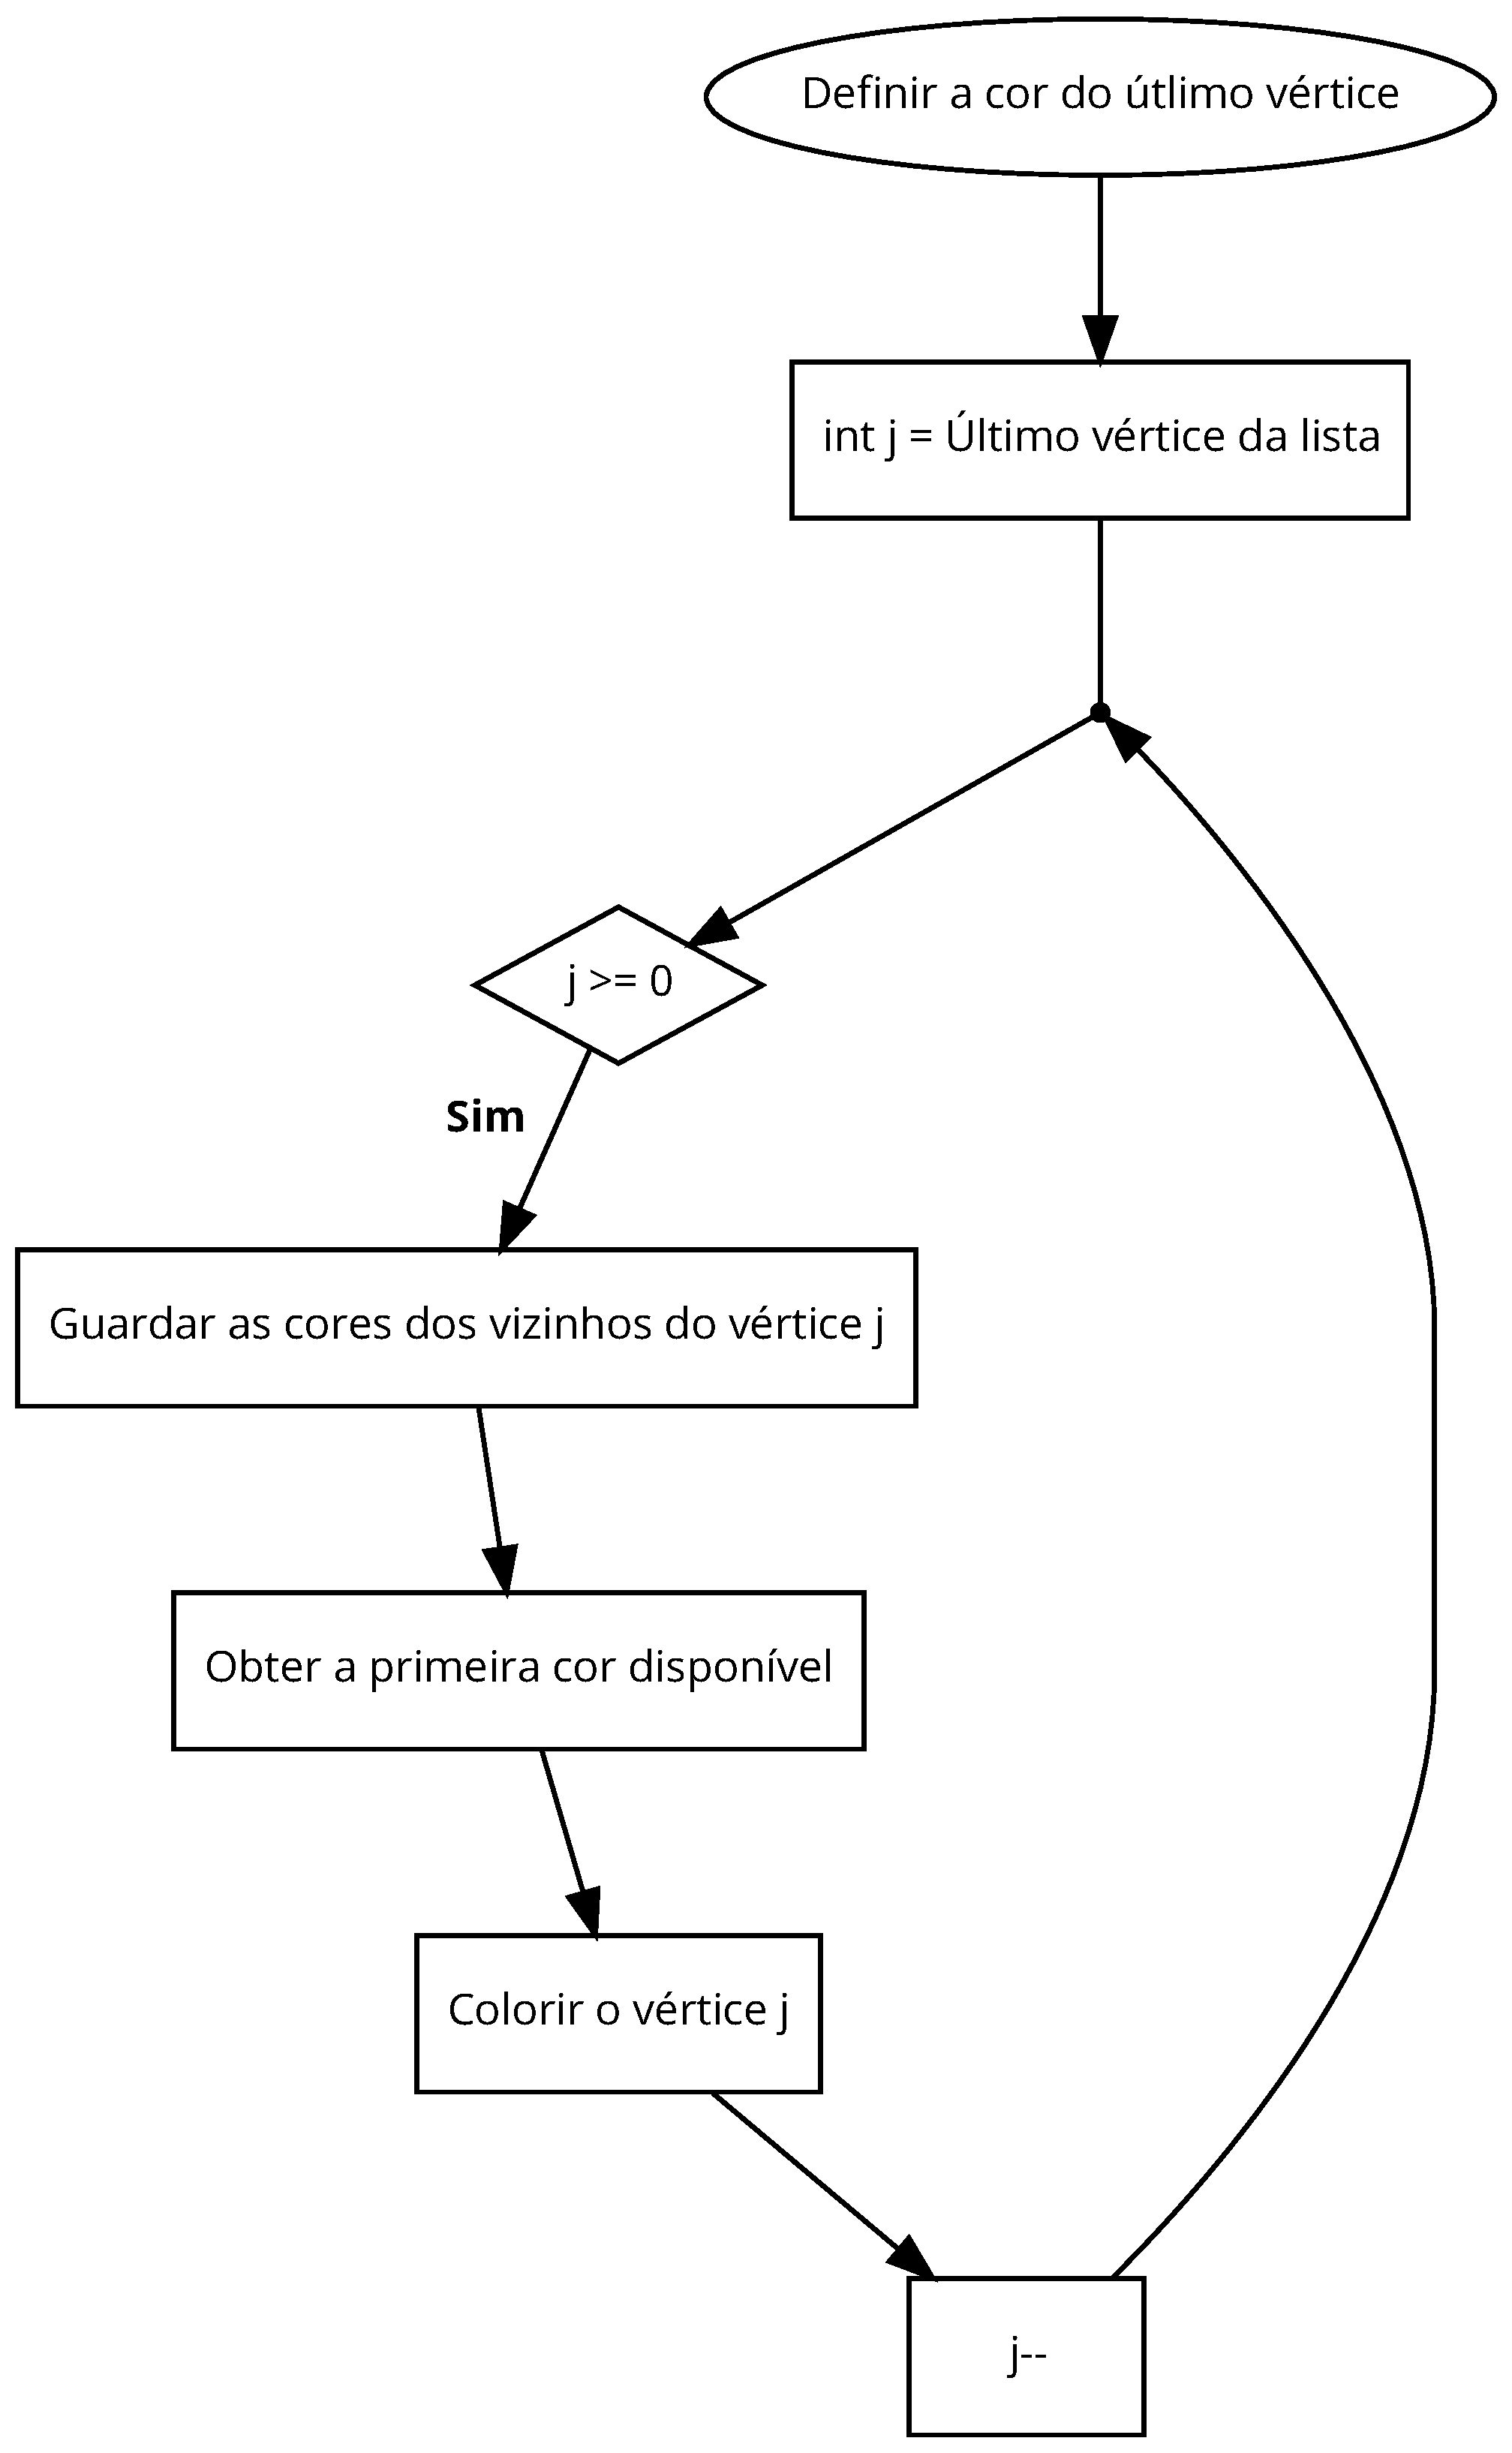
\includegraphics[scale=0.25]{img/colorizeVersion2.pdf}
    \caption{Colorização do grafo, versão 3}
    \label{fig:cV3}
\end{figure}

\begin{lstlisting}
    v3.setColorVertex(-1);
    for (int j = v3.getVertexList().size()-2; j >= 0; j--) {
        v3.saveNeighborColors(j);
        v3.setColorVertex(j);
    }
\end{lstlisting}

\section{\textit{Depth First Search} (DFS)}

Esta implementação recebe um objeto do tipo grafo (\textit{Graph.java}).
Quando invocada, a lista dos vértices do grafo.
Este objeto contém atributos como uma lista de vértices (\textit{vertexList}), \textit{orderIndex} que servirá para definir a ordem pela qual um vértice foi visitado (inicialmente contém o valor 0) e uma lista de vértices em espera para serem visitados (\textit{stack}).

\begin{lstlisting}
    graph.sortVertexByDegree();
    vertexList = graph.getVertexList();
\end{lstlisting}

O método \textit{getFirstNonVisitedVertex ()} verifica se existem algum vértice não visitado na lista. Caso se verifica então percorre os vértices contidos na lista e quando encontrar o primeiro vértice da lista não visitado, retorna-o.

\begin{figure}[H]
    \centering
        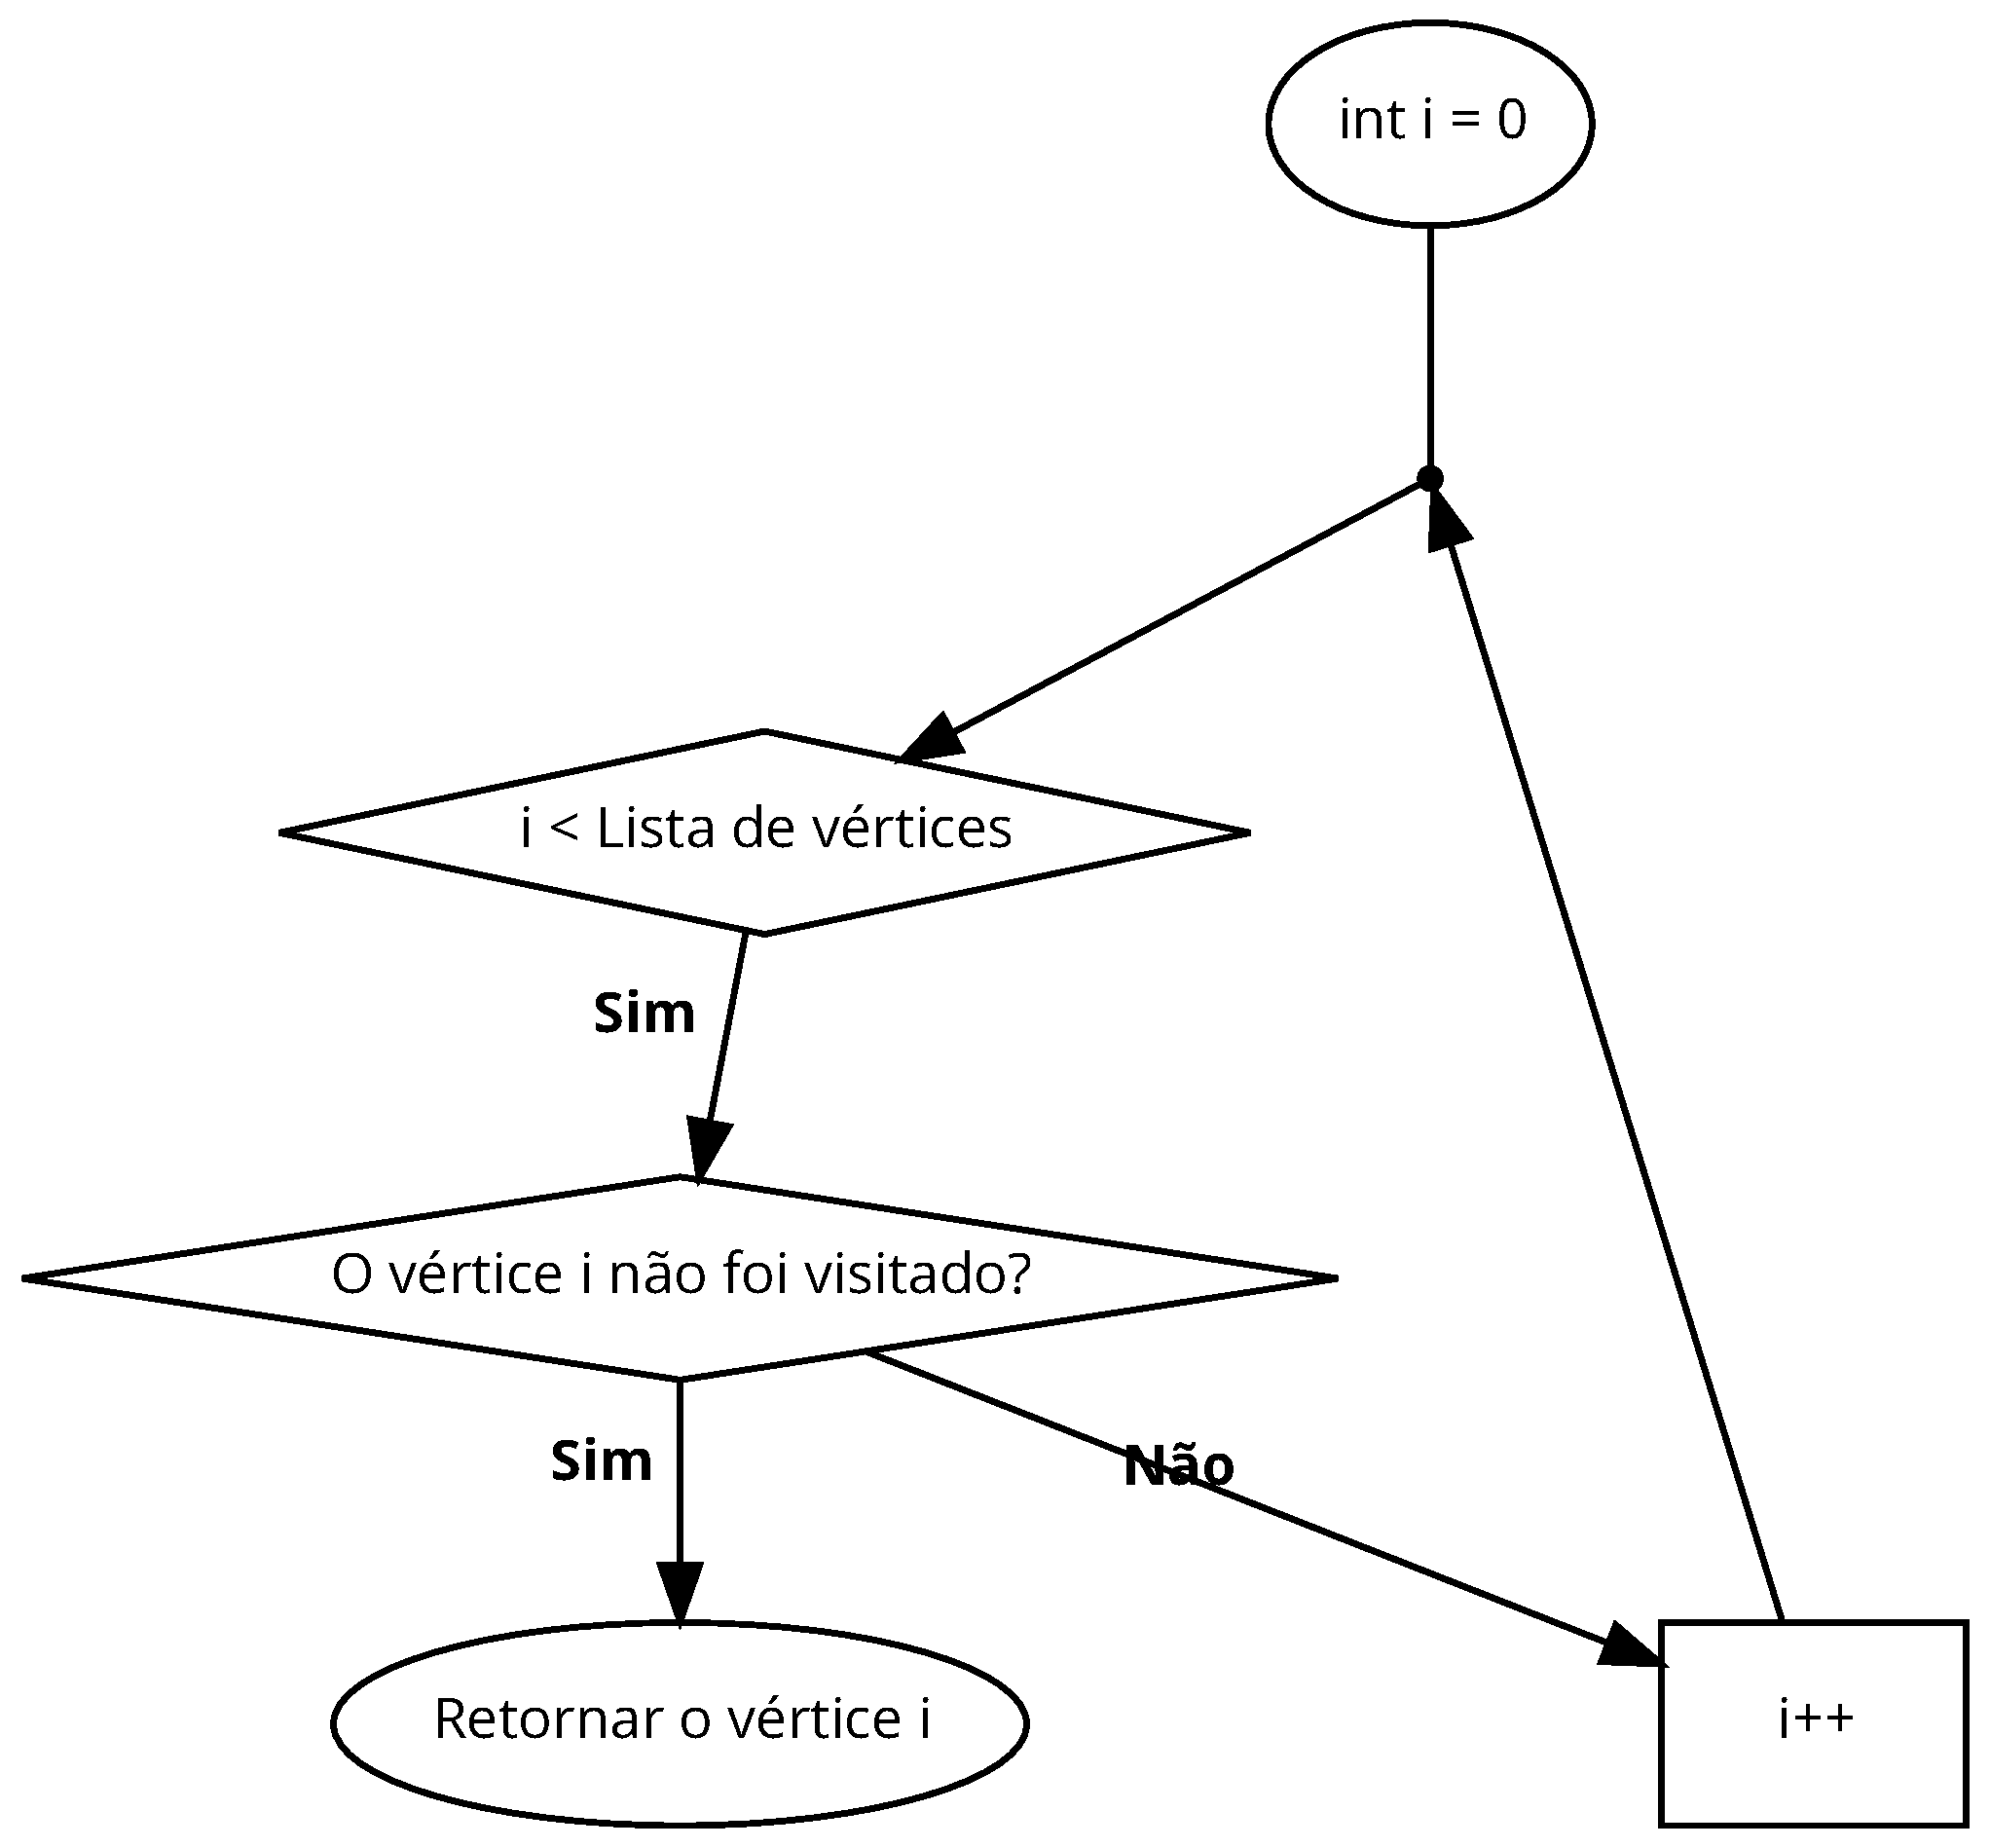
\includegraphics[scale=0.25]{img/getFirstNonVisitedVertex.pdf}
    \caption{Obter o primeiro vértice não visitado}
    \label{fig:gfnvv}
\end{figure}

\begin{lstlisting}
    for (int i = 0; i < vertexList.size(); i++)
        if (!vertexList.get(i).isVisited())
            return vertexList.get(i);
    return vertexList.get(0);
\end{lstlisting}

O método \textit{haveNonVisitedVertexes ()} verifica se a lista contém vértices não visitados.

\begin{figure}[H]
    \centering
        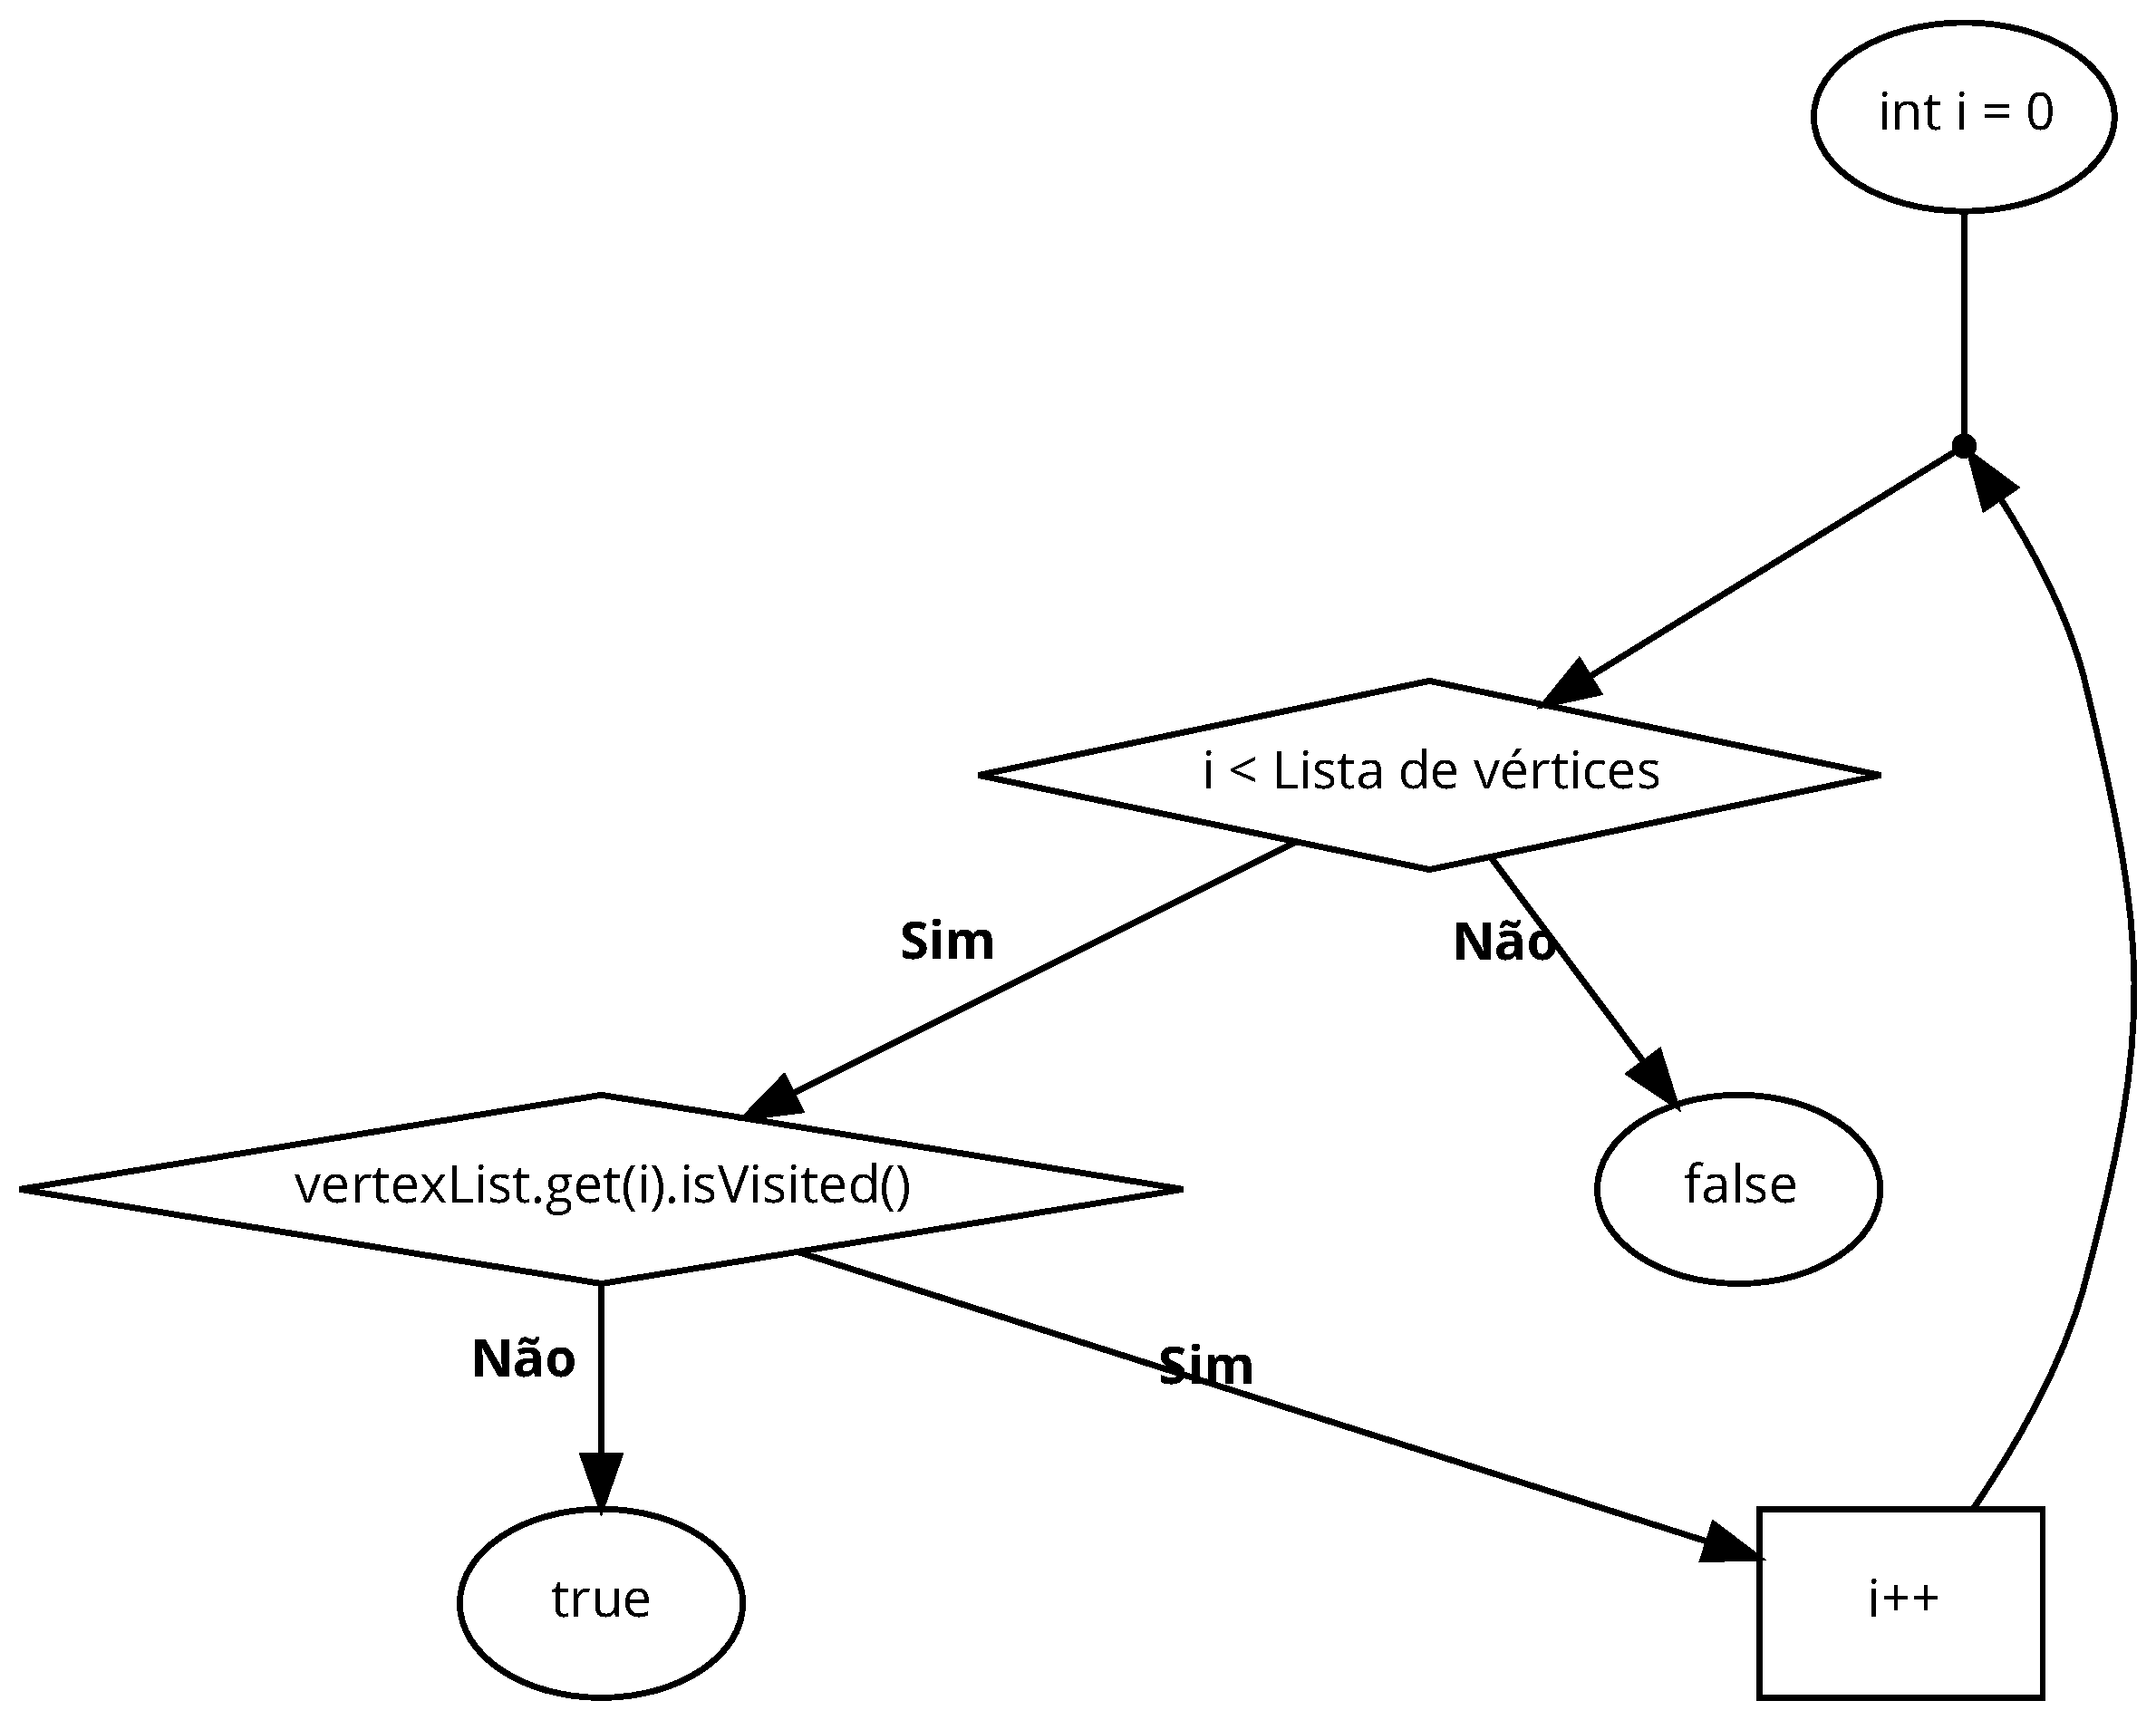
\includegraphics[scale=0.25]{img/haveNonVisitedVertexes.pdf}
    \caption{Verificação da existência de vértices não visitados}
    \label{fig:hnvv}
\end{figure}

\begin{lstlisting}
    for (int i = 0; i < vertexList.size(); i++)
        if (!vertexList.get(i).isVisited()) {
            return true;
        }
    return false;
\end{lstlisting}

O método \textit{setVisited (Vertex vertex)} recebe um vértice e define-o como visitado e atribui a ordem pela qual foi visitado. 

\begin{lstlisting}
    vertex.setVisited();
    setOrder(vertex);
\end{lstlisting}

O método \textit{getVisited (Vertex vertex)} retorna um valor booleano para determinar se o vértice \textit{vertex} já foi visitado anteriormente.

\begin{lstlisting}
    if (vertex.isVisited()) {
        return true;
    } else {
        return false;
    }
\end{lstlisting}

O método \textit{setOrder (Vertex vertex)} defina a ordem pela qual o vértice foi visitado e adiciona-o à \textit{stack} dos vértices em espera.

\begin{lstlisting}
    vertex.setOrder(++orderIndex);
    addToStack(vertex);    
\end{lstlisting}

O método \textit{addToStack (Vertex vertex)} adiciona à lista de espera o vértice vertex.

\begin{lstlisting}  
    stack.add(vertex);
\end{lstlisting}    

O método \textit{getStack ()} retorna a lista com os vértices em espera.

\begin{lstlisting}
    return stack;
\end{lstlisting}

O método \textit{getTopStack ()} retorna o primeiro vértice na lista dos vértices em espera.

\begin{lstlisting}
    return stack.pop();
\end{lstlisting}

O método \textit{getAllSucessors (Vertex vertex)} retorna um iterador dos sucessores do vértice \textit{vertex}.

\begin{lstlisting}
    return vertex.getSucessorList().listIterator();
\end{lstlisting}

O método \textit{getNextSucessor (Iterator<Integer> neighbors)} retorna o próximo sucessor (vértice) do vértice identificado por \textit{neighbors}.

\begin{lstlisting}
    return vertexList.get(neighbors.next());    
\end{lstlisting}

O método \textit{haveNonVisitedPredecessors (Vertex vertex)} verifica se o vértice \textit{vertex} tem predecessores visitados. Para tal, percorre a lista de predecessores do vértice \textit{vertex} e quando encontrar (se encontrar) um vértice predecessor não visitado retorna \textit{true}.

\begin{figure}[H]
    \centering
        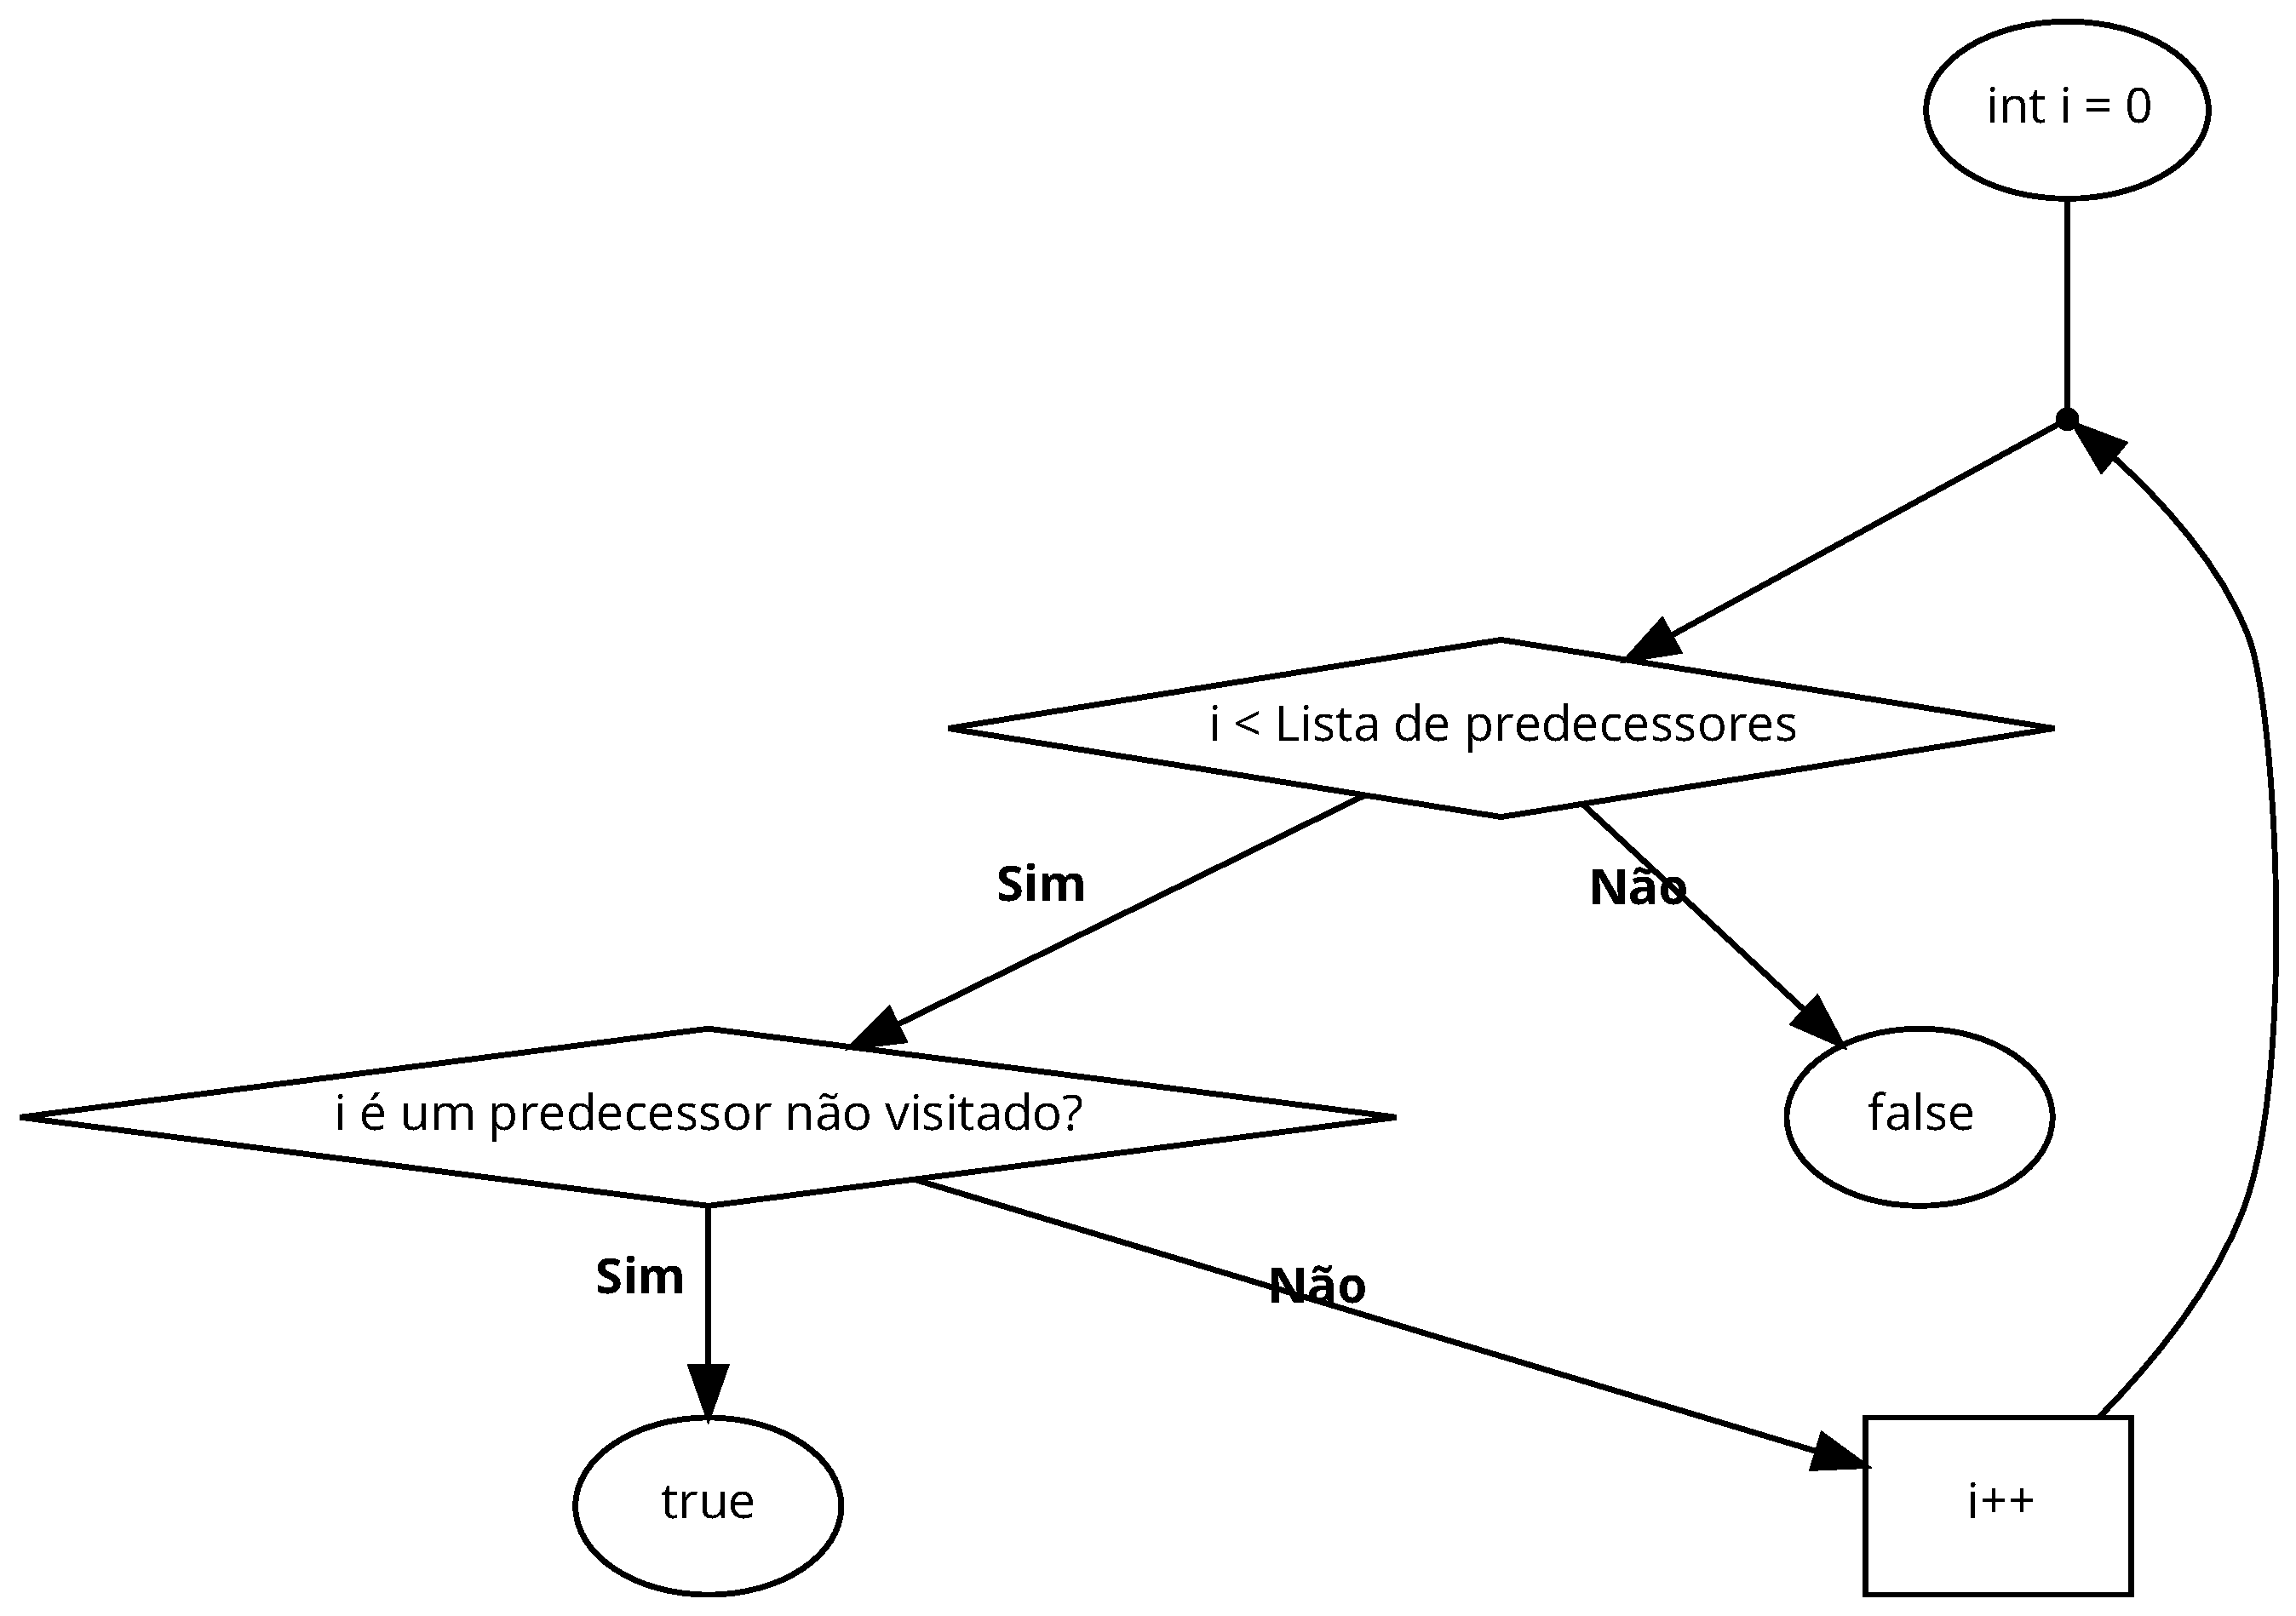
\includegraphics[scale=0.25]{img/haveNonVisitedPredecessors.pdf}
    \caption{Verificação da existência de predecessores não visitados}
    \label{fig:hnvp}
\end{figure}

\begin{lstlisting}
    for (int i = 0; i < vertex.getPredecessorList().size(); i++) {
        if (!vertexList.get(vertex.getPredecessorList().get(i)).isVisited())
            return true;
    }
    return false;
\end{lstlisting}

\subsection*{Algoritmo}

Em suma, a implementação final do algoritmo consiste na verificação da existência de algum vértice não visitado. No caso de existir obtém o primeiro vértice da lista que ainda não foi visitado, definindo-o seguidamente como visitado e adicionando-o à lista de espera. Após concluido este processo vão analisar se existem vértices na lista de espera, obtendo os visinhos primeiro vértice disponível. Enquanto existirem vizinhos obtém o seu sucessor, verificando se já foi visitado e se contém predecessores não visitados. No caso de esta condição se verificar, define-o como visitado e volta à verificação da existência de mais vizinhos.
Este processo repete-se enquanto houverem vértices não visitaos ou existirem vértices na lista de espera.

\begin{figure}[H]
    \centering
        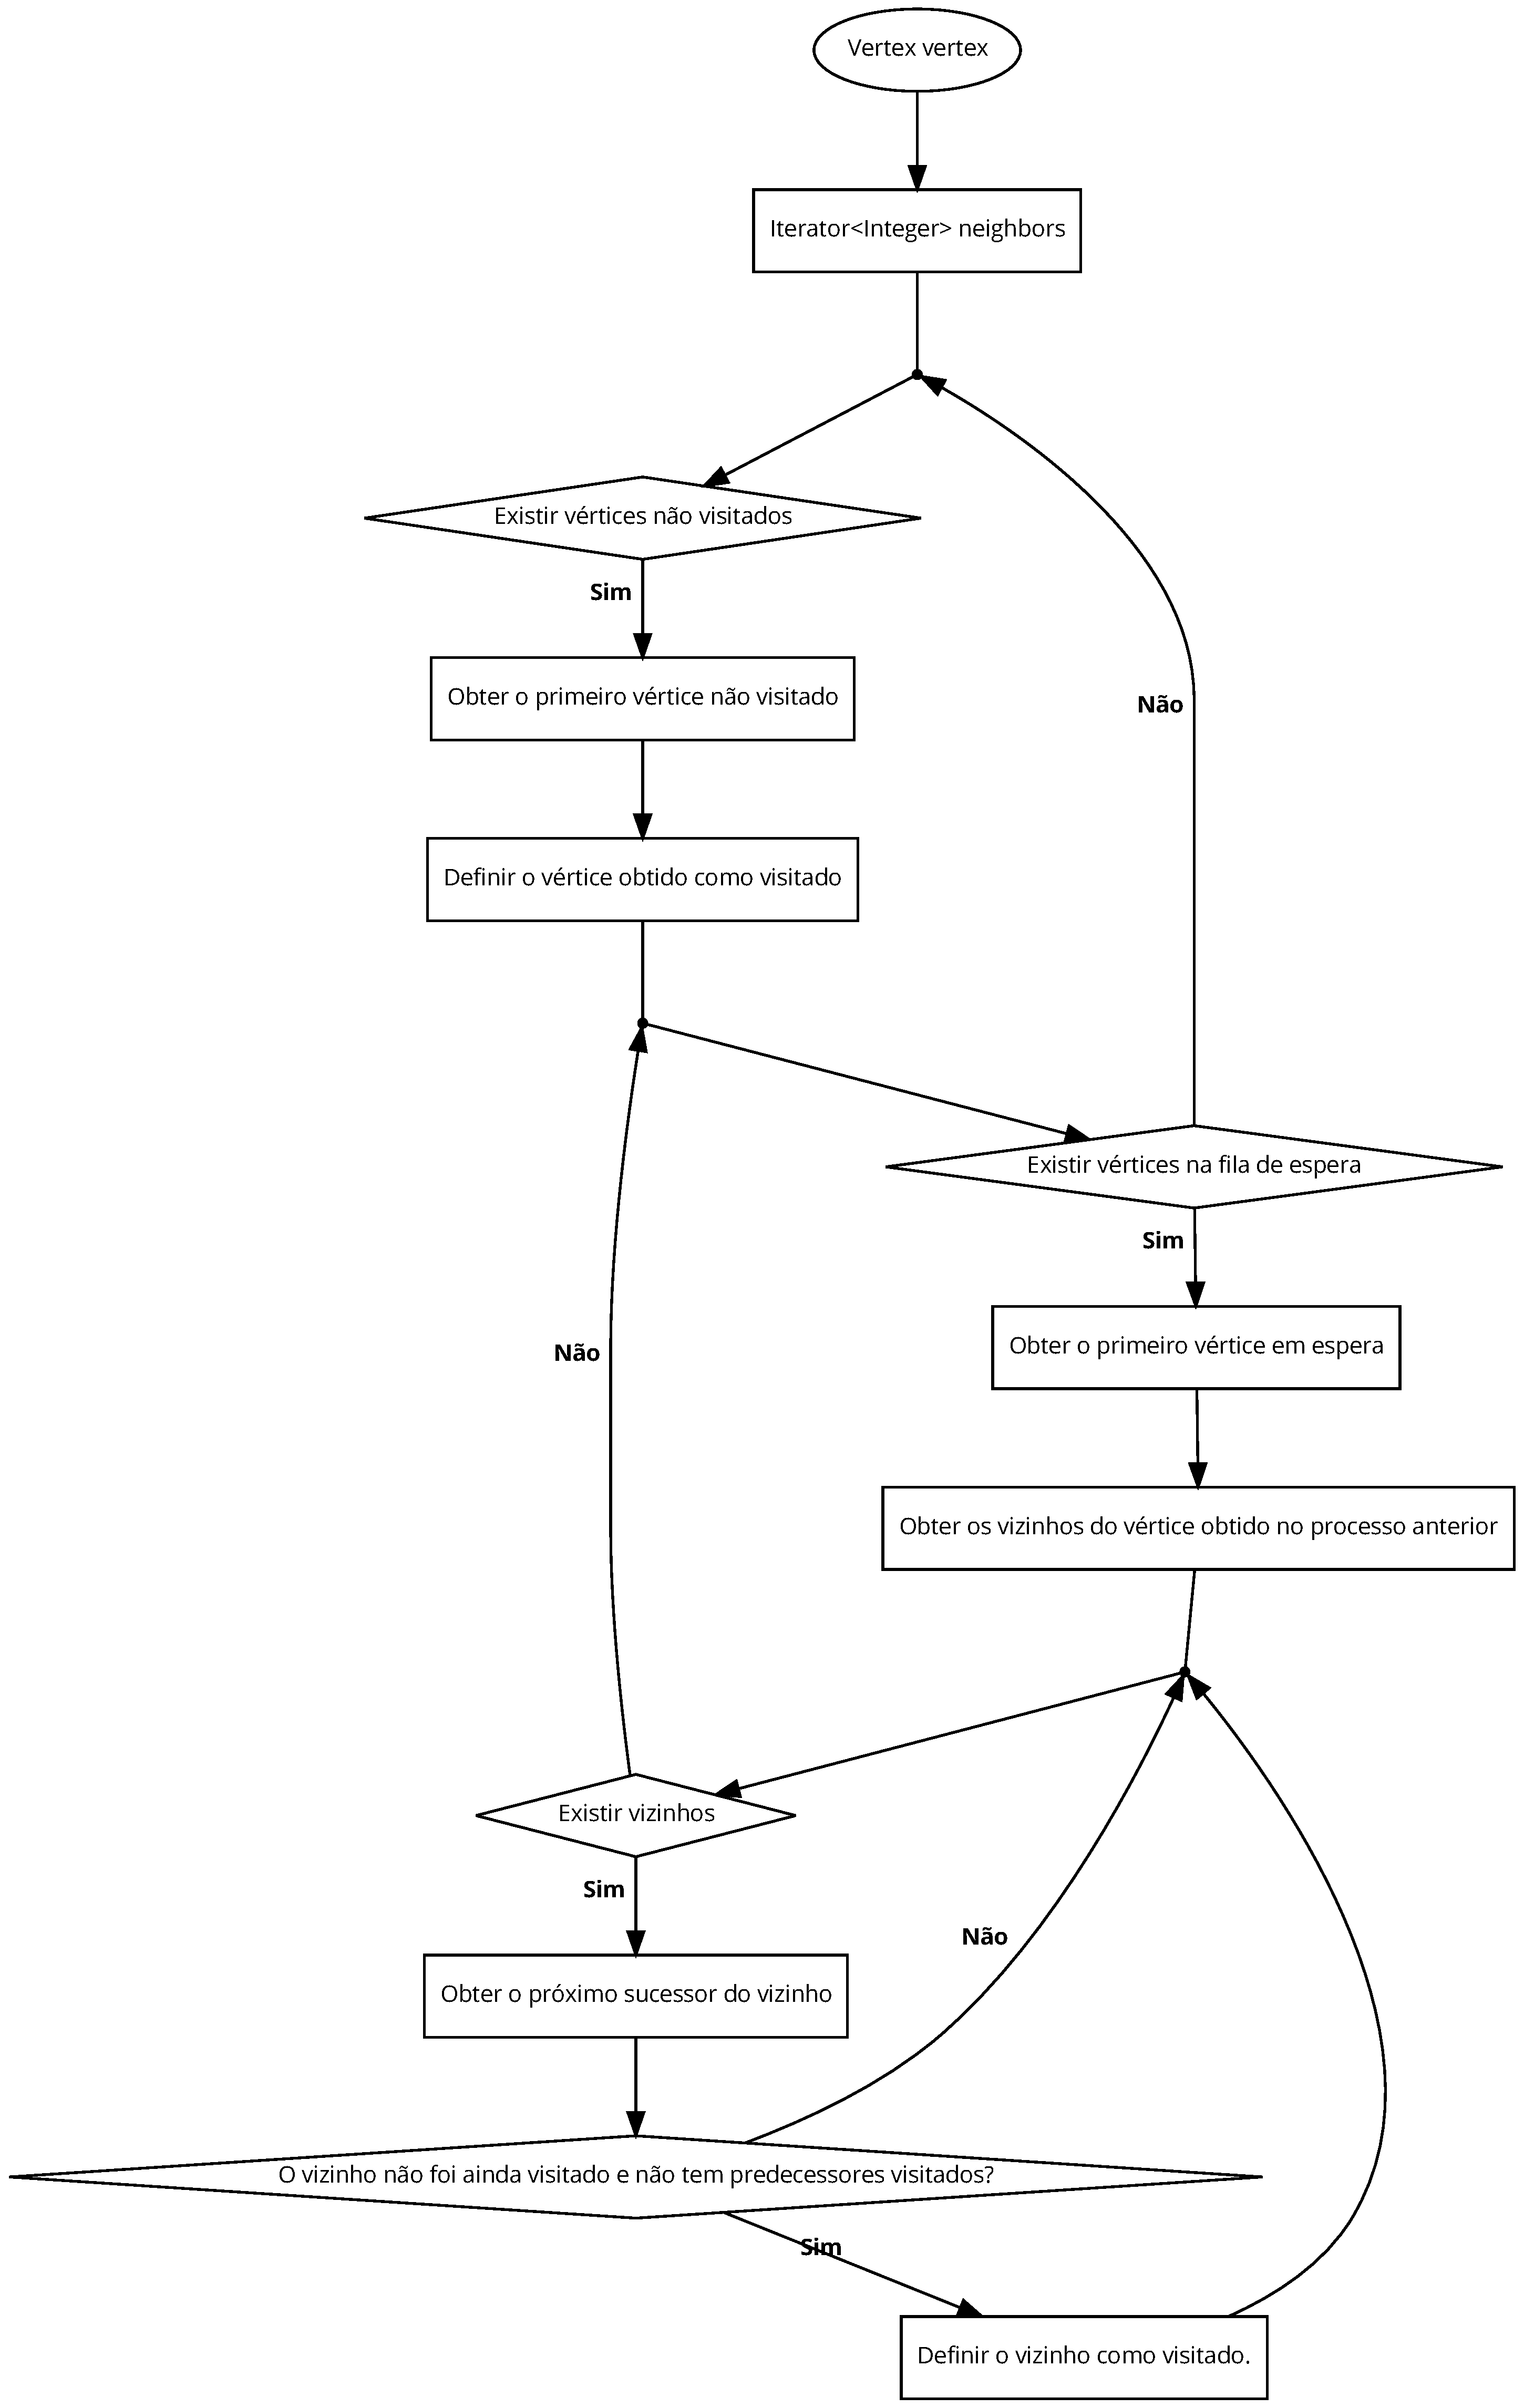
\includegraphics[scale=0.16]{img/dfs.pdf}
    \caption{Algoritmo \textit{Depth First Search}}
    \label{fig:dfsAl}
\end{figure}

\begin{lstlisting}
    Vertex vertex;
    Iterator<Integer> neighbors;
    while (dfs.haveNonVisitedVertexes()) {
        vertex = dfs.getFirstNonVisitedVertex();
        dfs.setVisited(vertex);
        while (dfs.getStack().size() != 0) {
            vertex = dfs.getTopStack();
            neighbors = dfs.getAllSucessors(vertex);
            while (neighbors.hasNext()) {
                Vertex n = dfs.getNextSucessor(neighbors);
                if (!dfs.getVisited(n) && !dfs.haveNonVisitedPredecessors(n))
                    dfs.setVisited(n);
            }
        }
    }
\end{lstlisting}

\chapter{Resolução dos exercícios (Análise e resultados)}

\section{Exercício 1}

Nos grafos apresentados nesta secção, o número em cada vértice representa o seu id.

\subsection*{Matriz $H$}

Consideremos a matriz $H$. Aplicamos o algoritmo \textit{ColorizeVersion1.java} à matriz $H$.

A coloração obtida é a representada no seguinte grafo:

\begin{figure}[H]
    \centering
        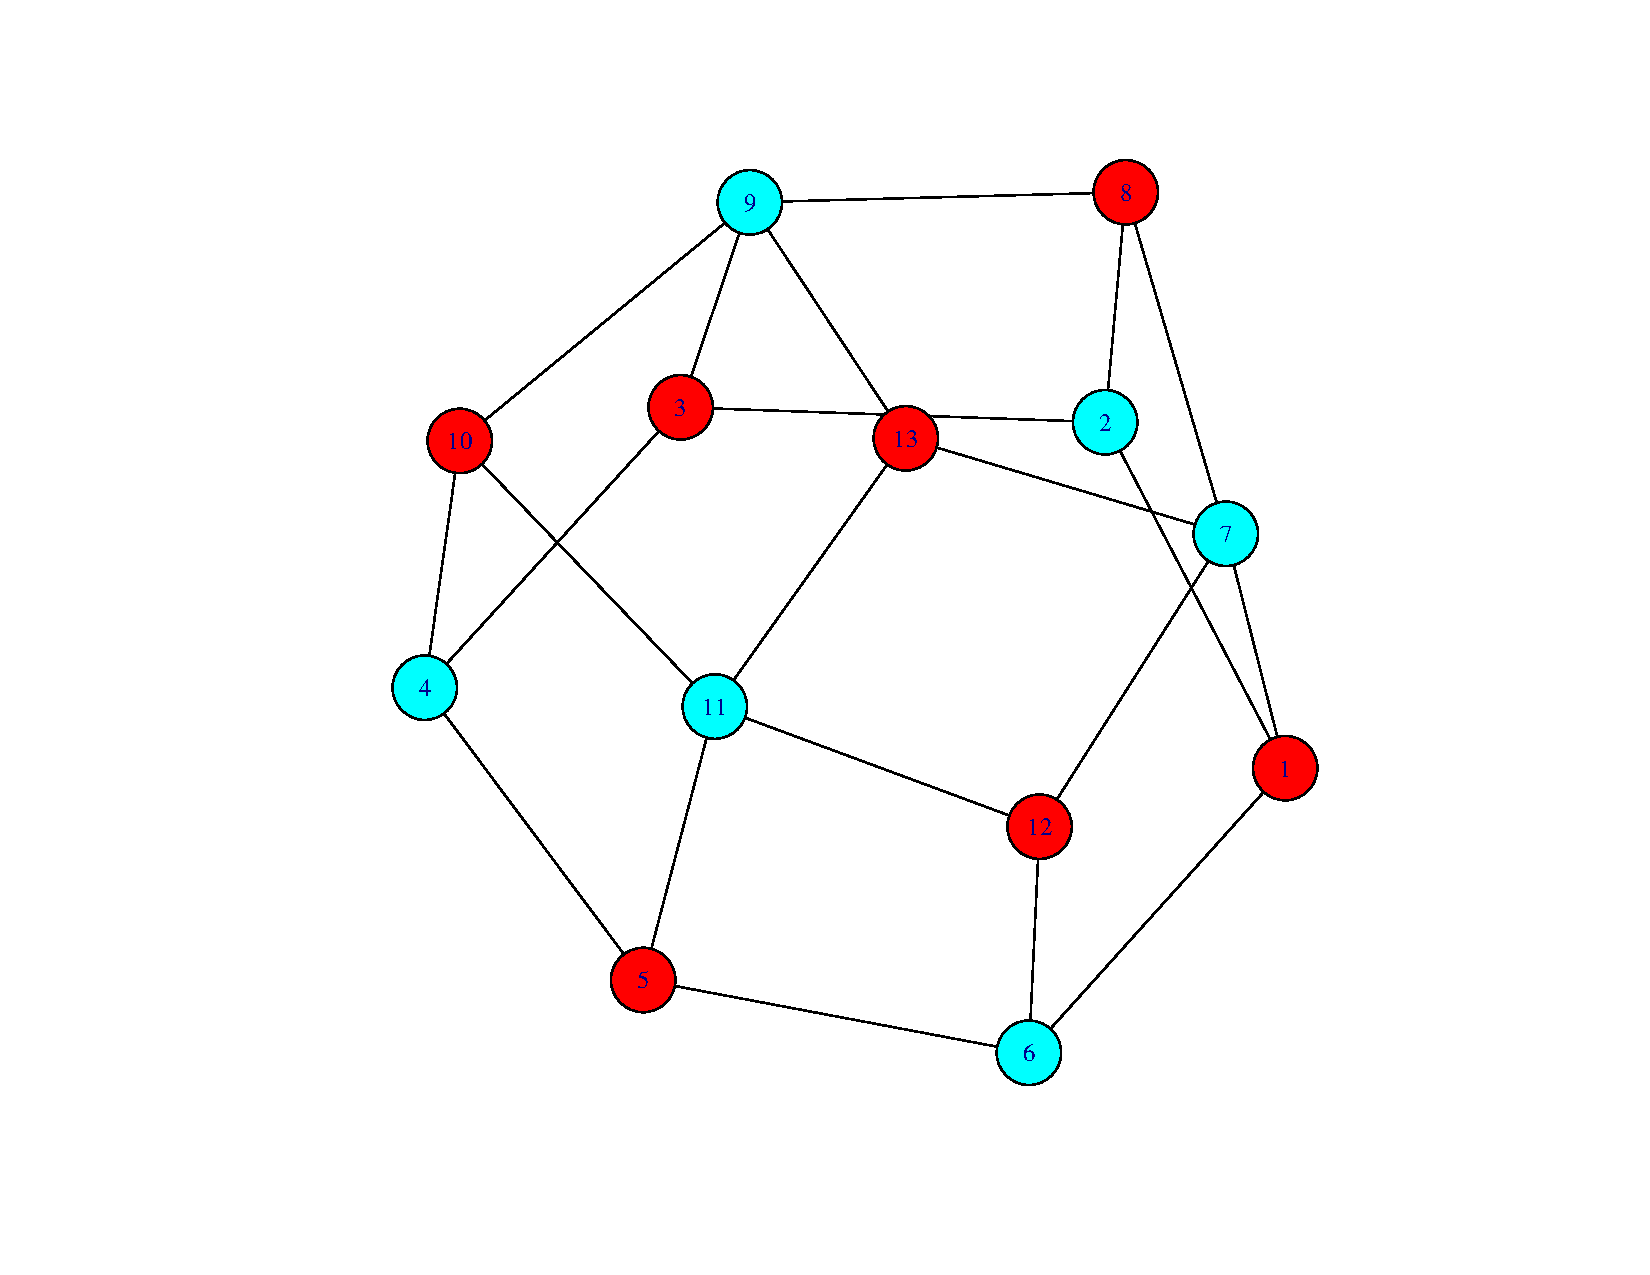
\includegraphics[scale=0.25]{img/v1H.pdf}
    \caption{Grafo H, coloração 1}
    \label{fig:v1H}
\end{figure}

Aplicando a versão 2 e 3 do algoritmo de coloração dos vértices, obtemos os seguintes resultados:

\begin{figure}[H]
    \centering
    \begin{minipage}{.5\textwidth}
      \centering
      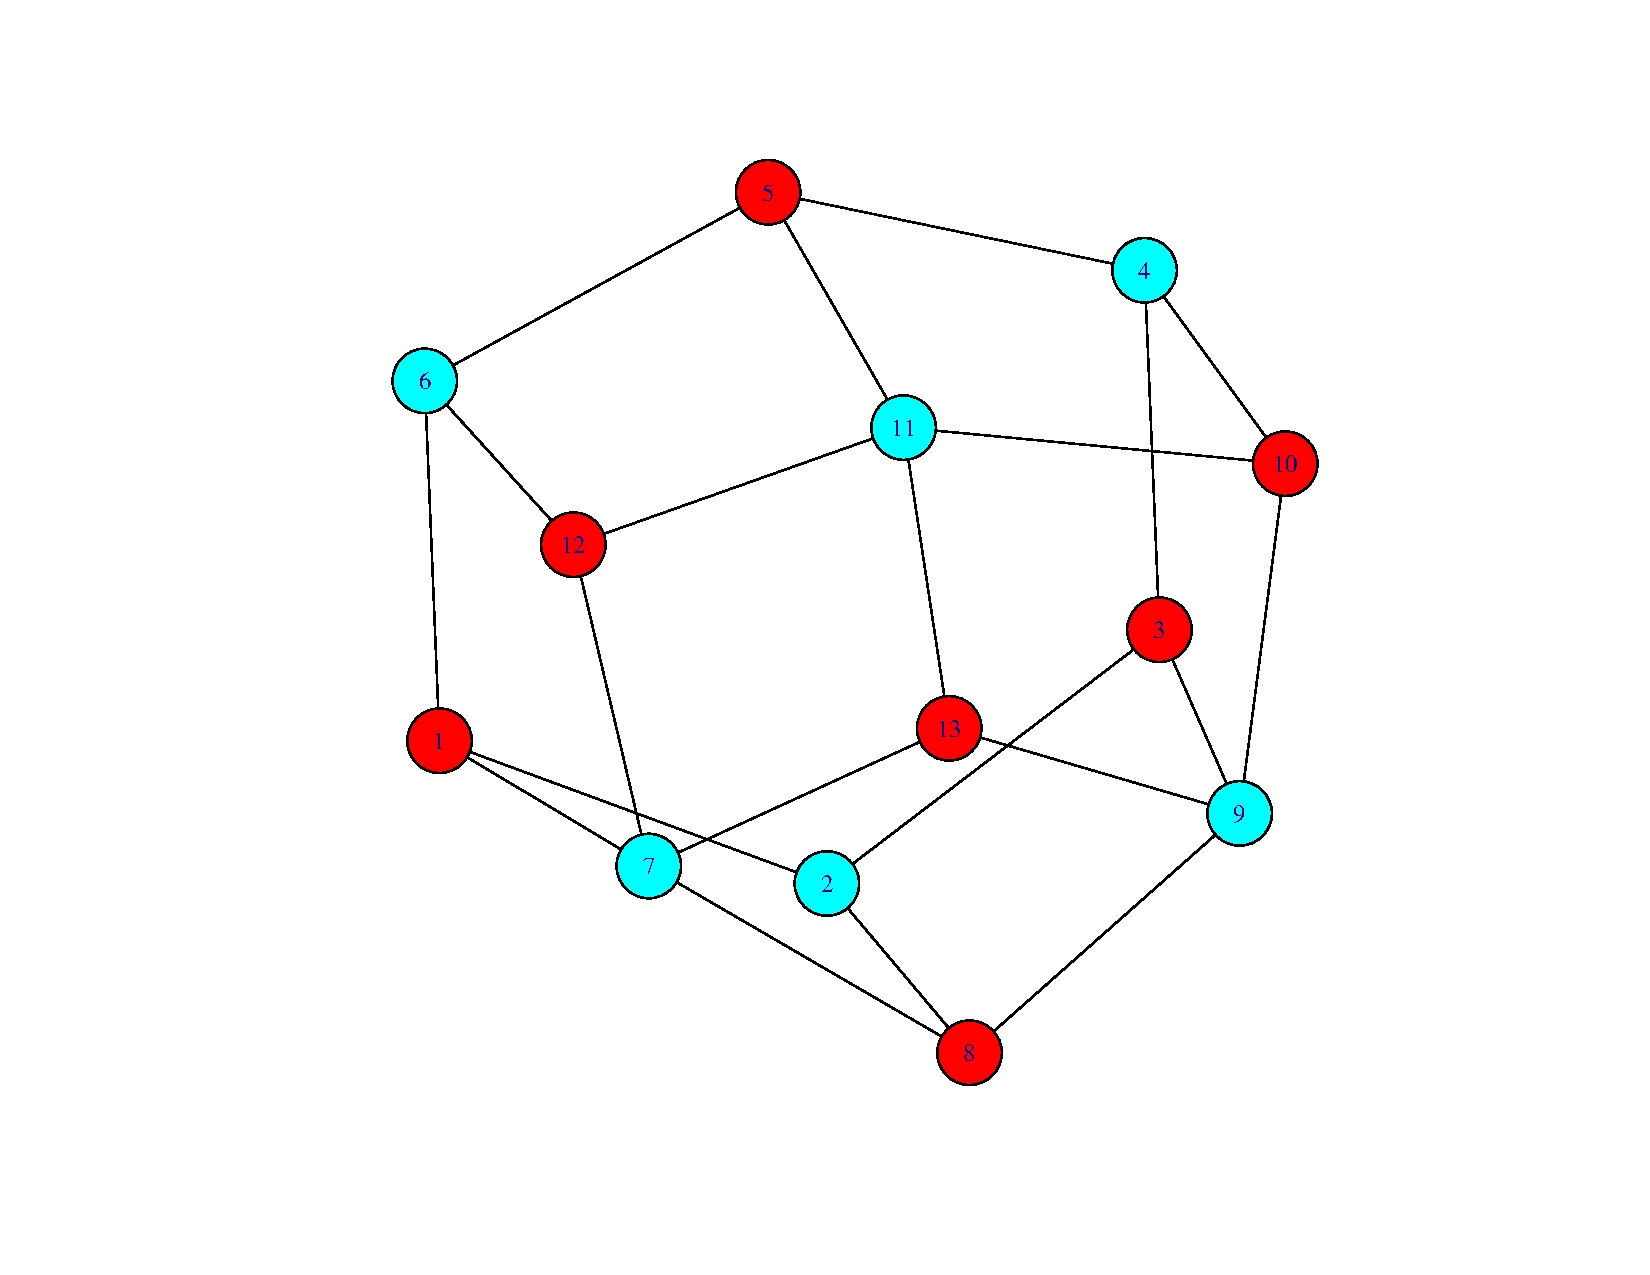
\includegraphics[scale=0.25]{img/v2H.pdf}
      \captionof{figure}{Grafo H, coloração 2}
      \label{fig:v2H}
    \end{minipage}%
    \begin{minipage}{.5\textwidth}
      \centering
      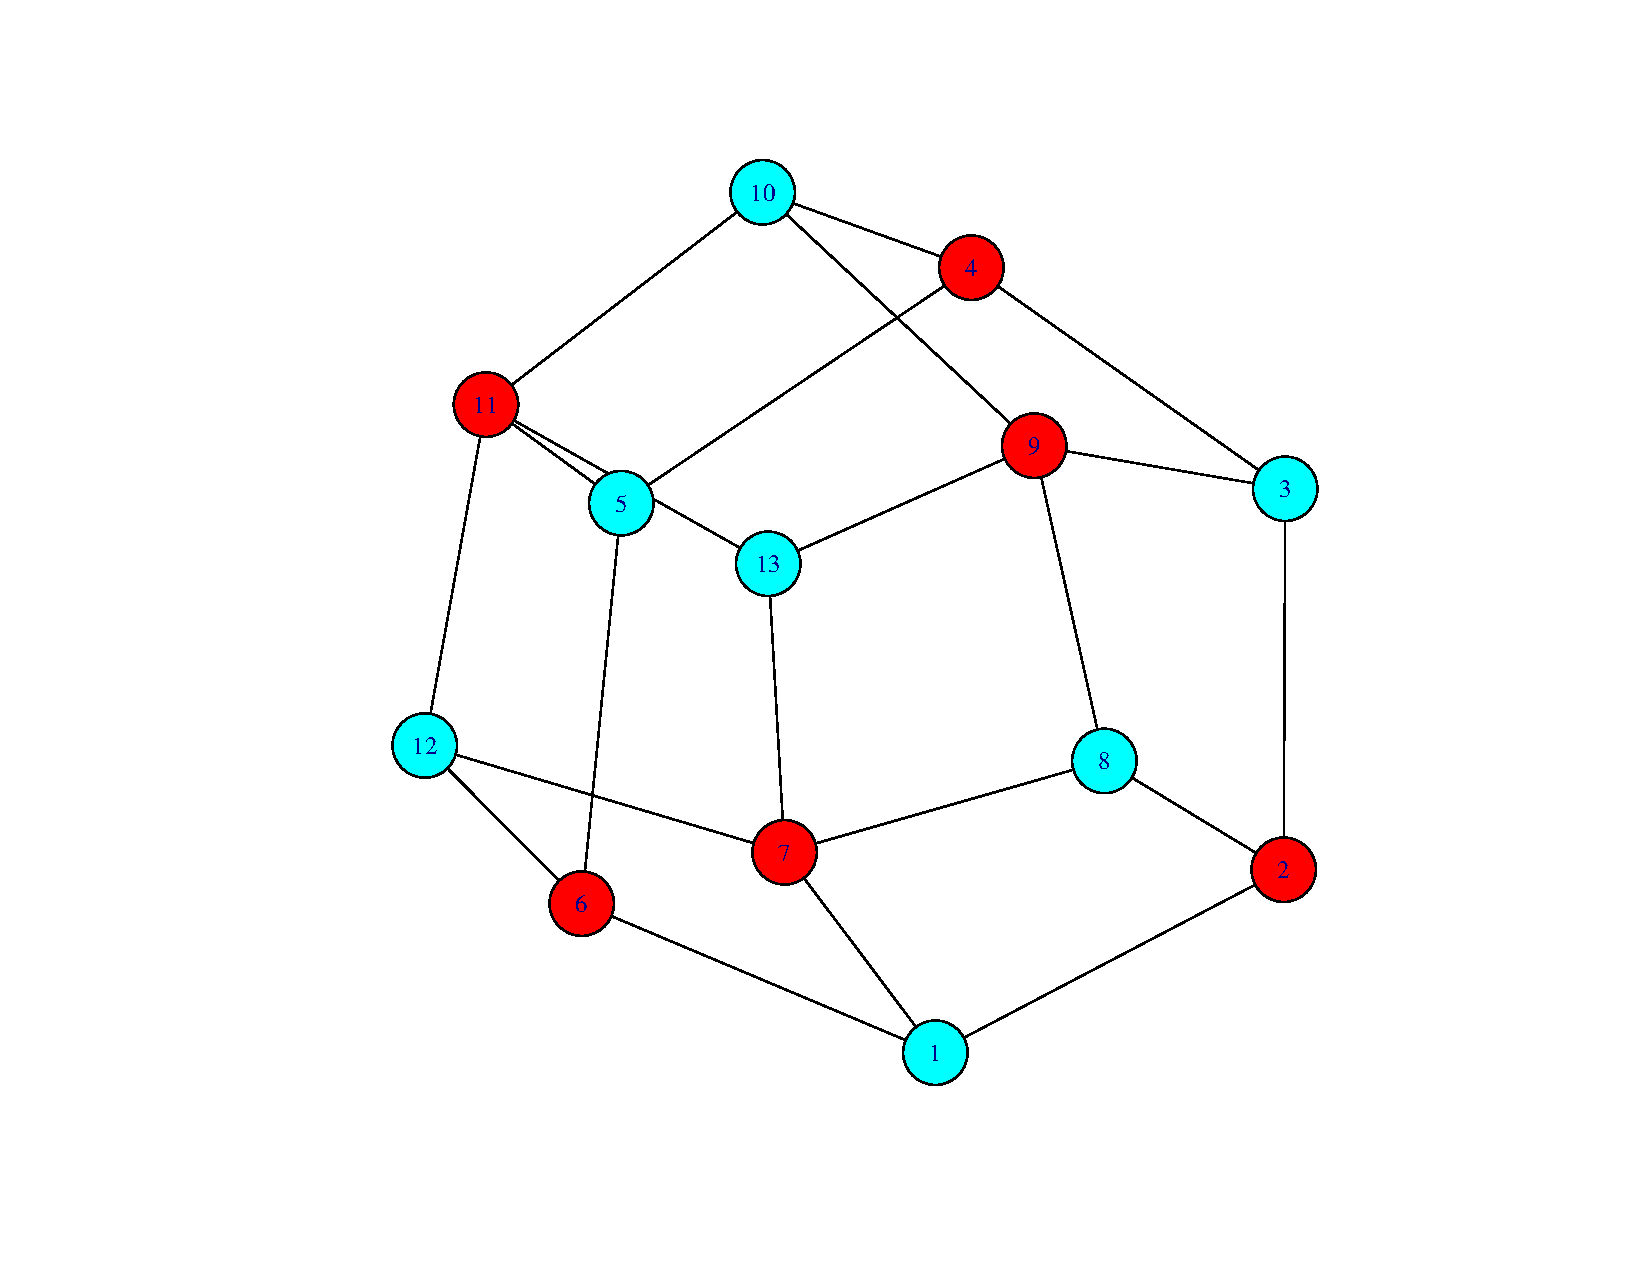
\includegraphics[scale=0.25]{img/v3H.pdf}
      \captionof{figure}{Grafo H, coloração 3}
      \label{fig:v3H}
    \end{minipage}
\end{figure}

Analisando os grafos obtidos, podemos ver que neste caso o algoritmo 1, 2 e 3 retornam colorações iguais, a menos de uma alteração das cores.

\subsection*{Matriz $J$}

Consideremos a matriz $J$. Aplicamos o algoritmo \textit{ColorizeVersion1.java} à matriz $J$.

A coloração obtida é a representada no seguinte grafo:

\begin{figure}[H]
    \centering
        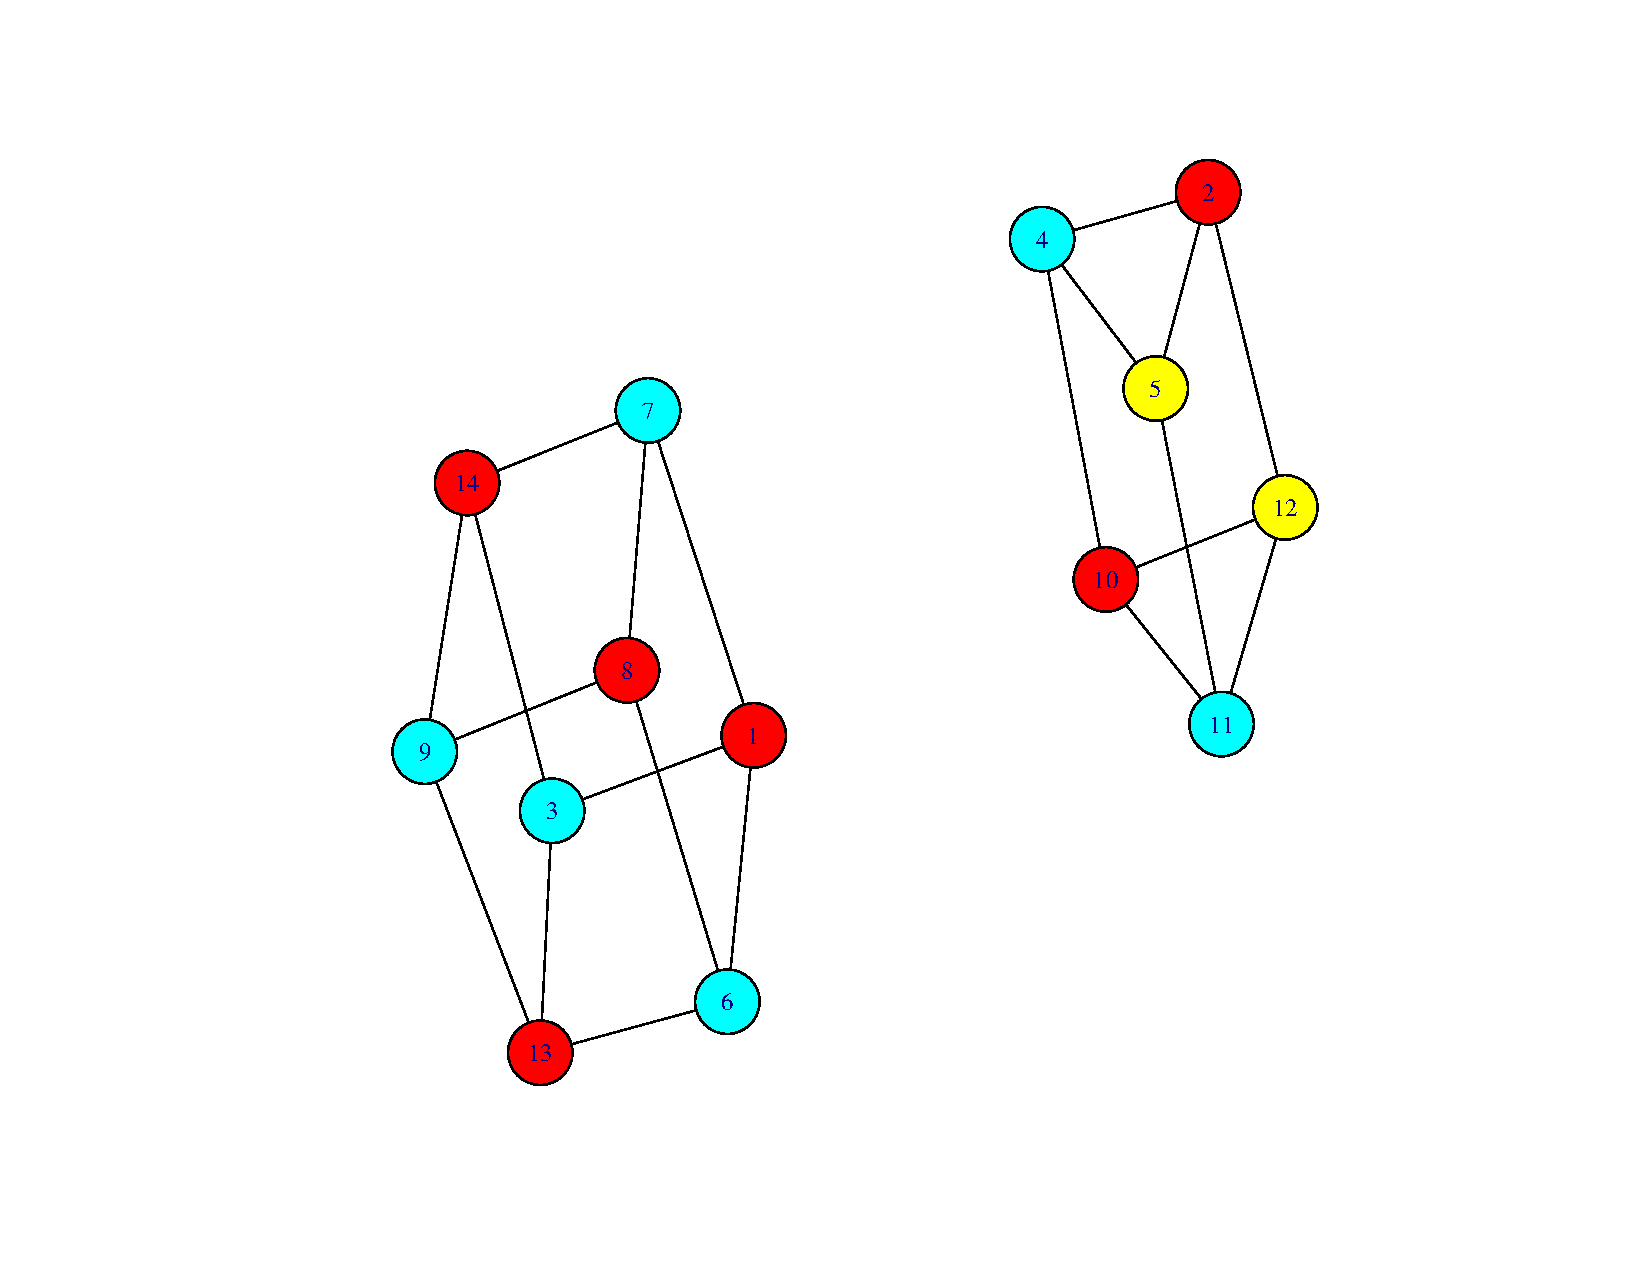
\includegraphics[scale=0.25]{img/v1J.pdf}
    \caption{Grafo J, coloração 1}
    \label{fig:v1J}
\end{figure}

Aplicando a versão 2 e 3 do algoritmo de coloração dos vértices, obtemos os seguintes resultados:

\begin{figure}[H]
    \centering
    \begin{minipage}{.5\textwidth}
      \centering
      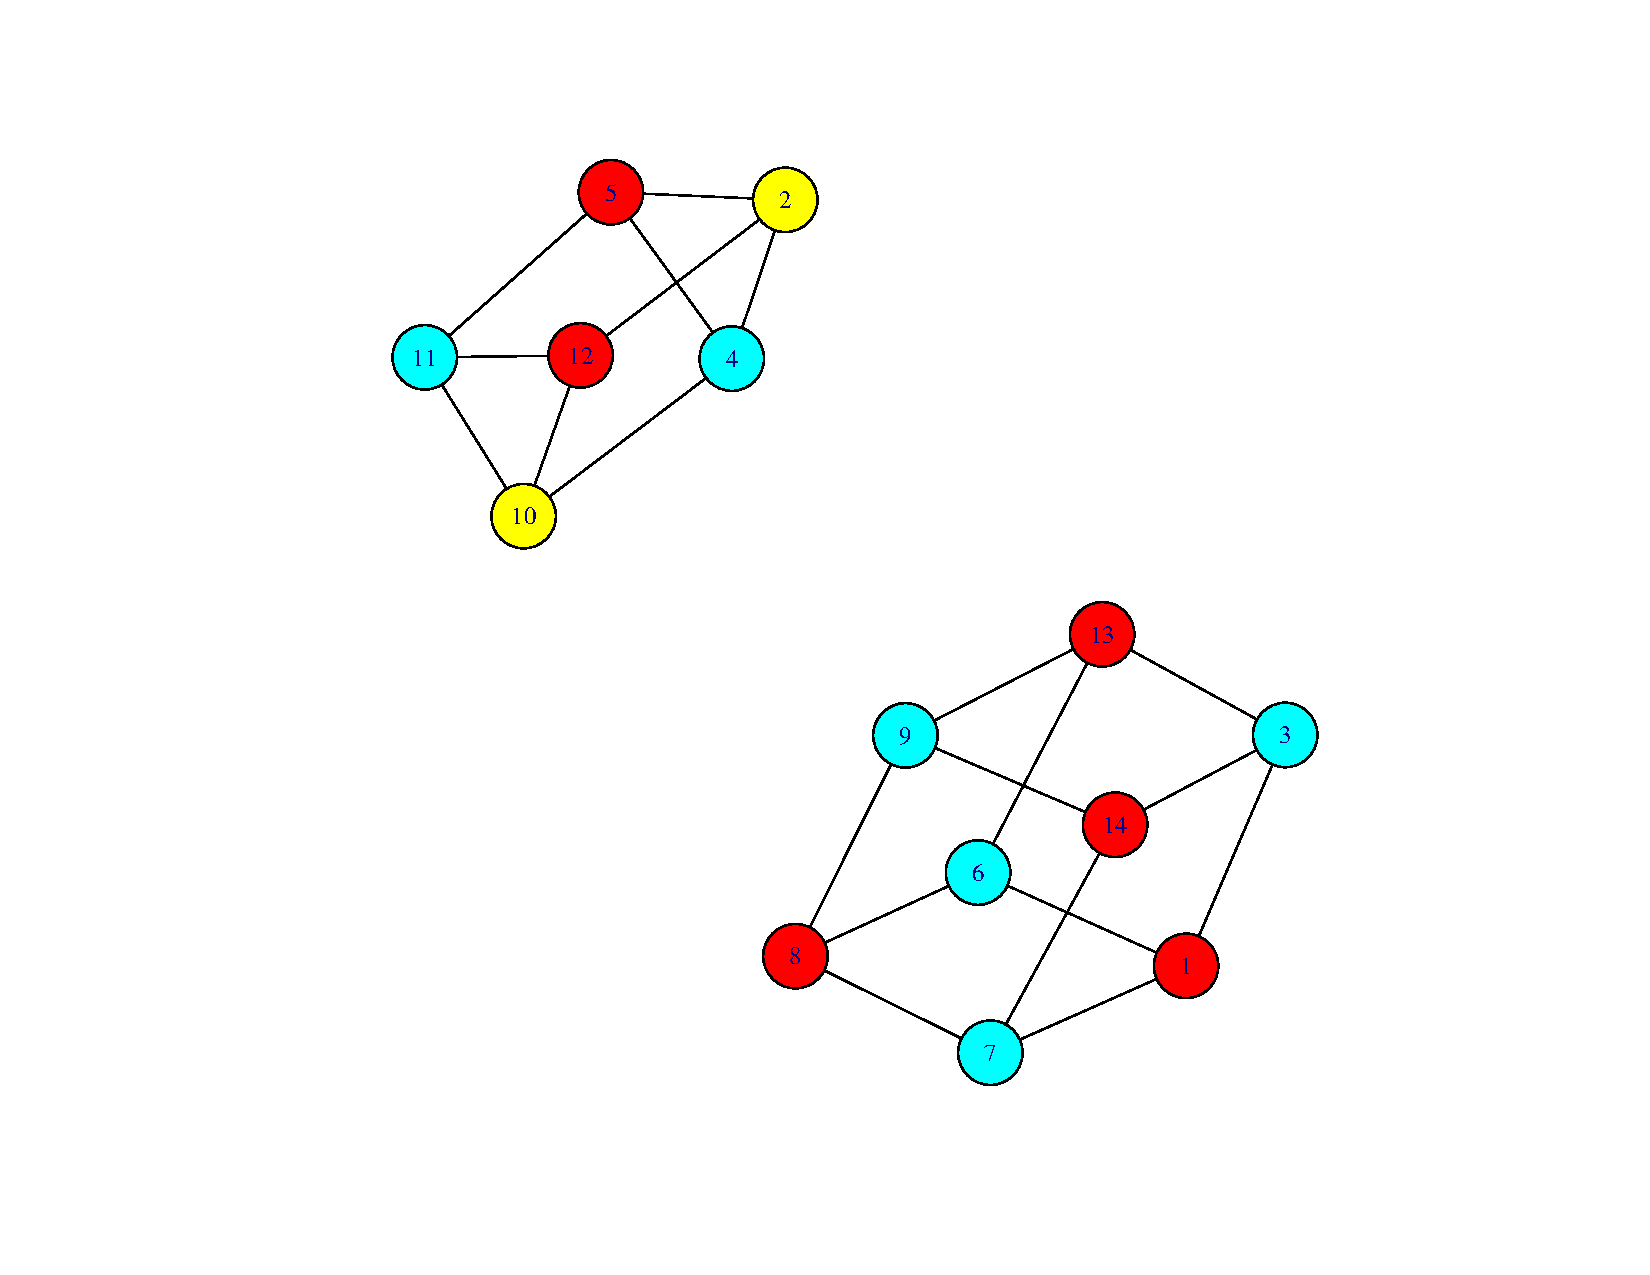
\includegraphics[scale=0.25]{img/v2J.pdf}
      \captionof{figure}{Grafo J, coloração 2}
      \label{fig:v2J}
    \end{minipage}%
    \begin{minipage}{.5\textwidth}
      \centering
      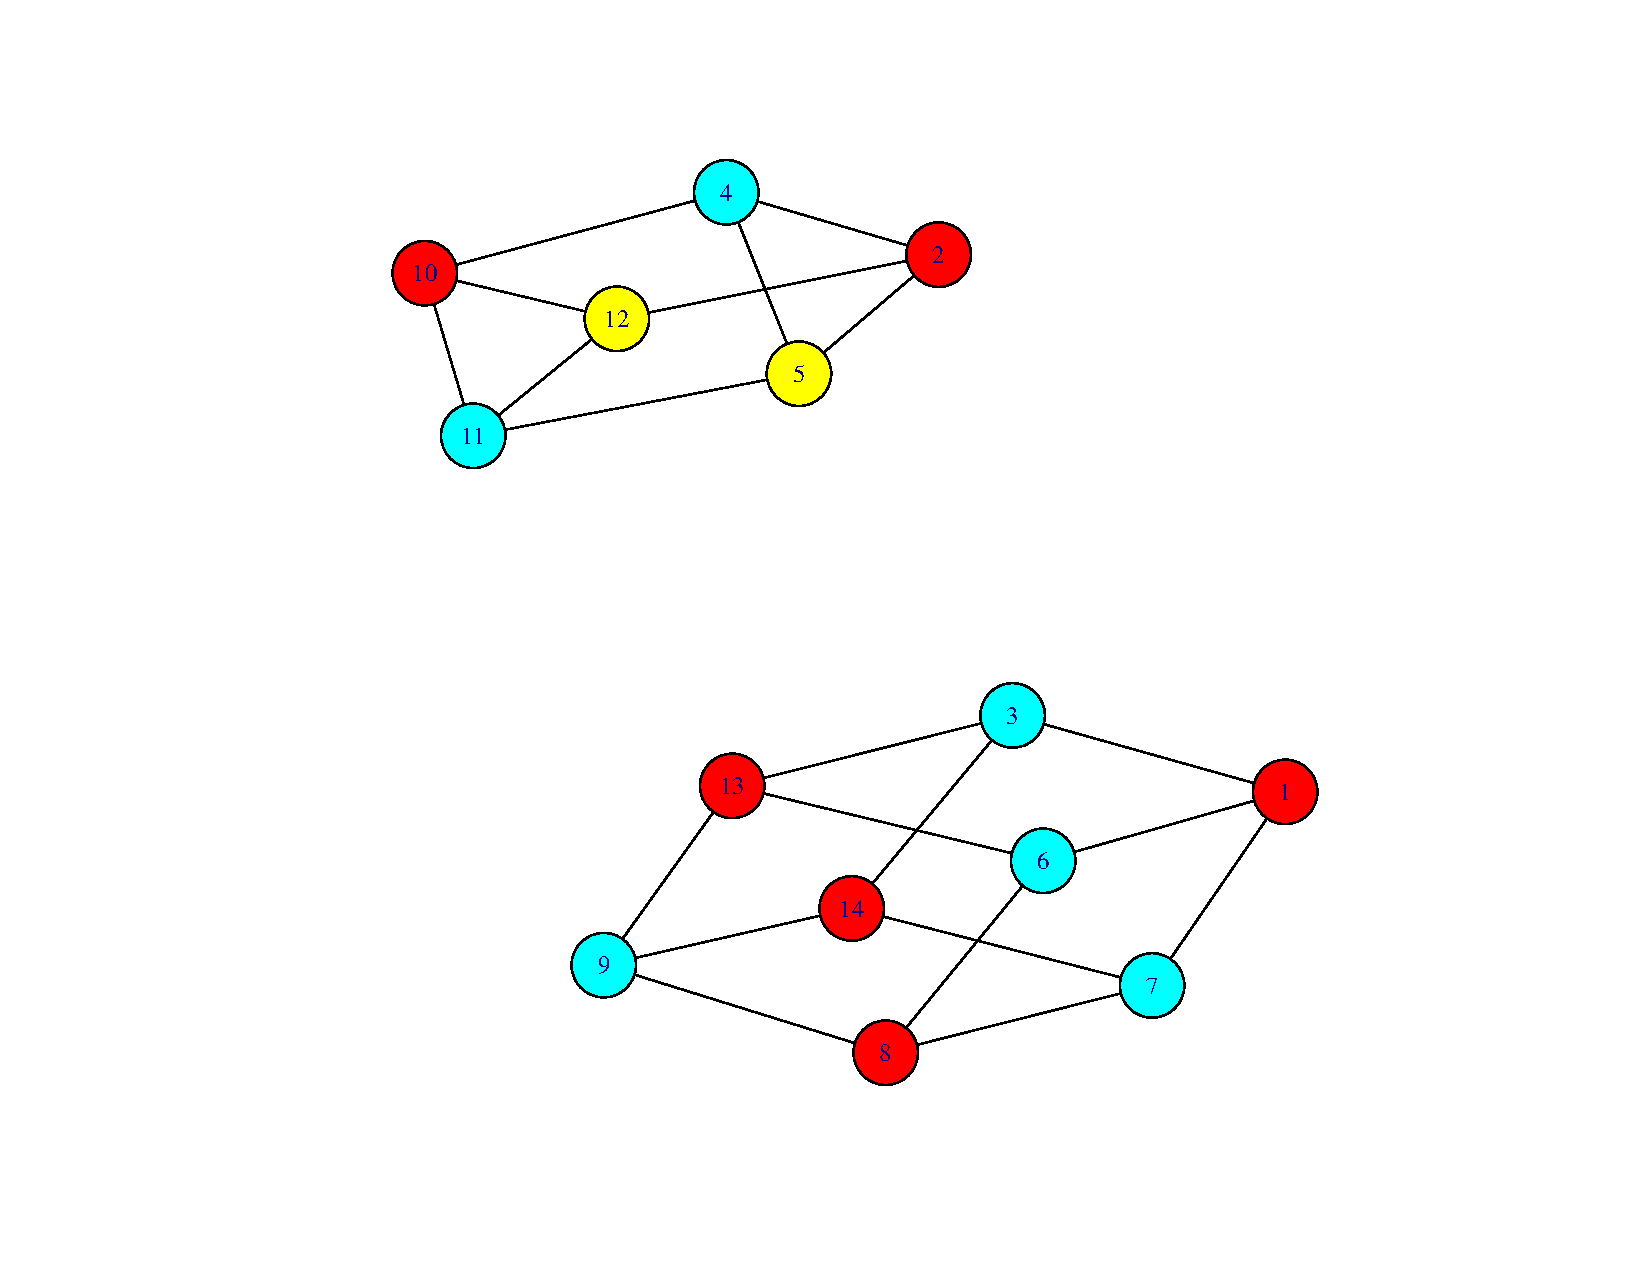
\includegraphics[scale=0.25]{img/v3J.pdf}
      \captionof{figure}{Grafo J, coloração 3}
      \label{fig:v3J}
    \end{minipage}
\end{figure}

Analisando os grafos obtidos, podemos ver que neste caso o algoritmo 1, 2 e 3 retornam colorações equivalentes.

\subsection*{Matriz $M$}

Consideremos a matriz $M$. Aplicamos o algoritmo \textit{ColorizeVersion1.java} à matriz $M$.

A coloração obtida é a representada no seguinte grafo:

\begin{figure}[H]
    \centering
        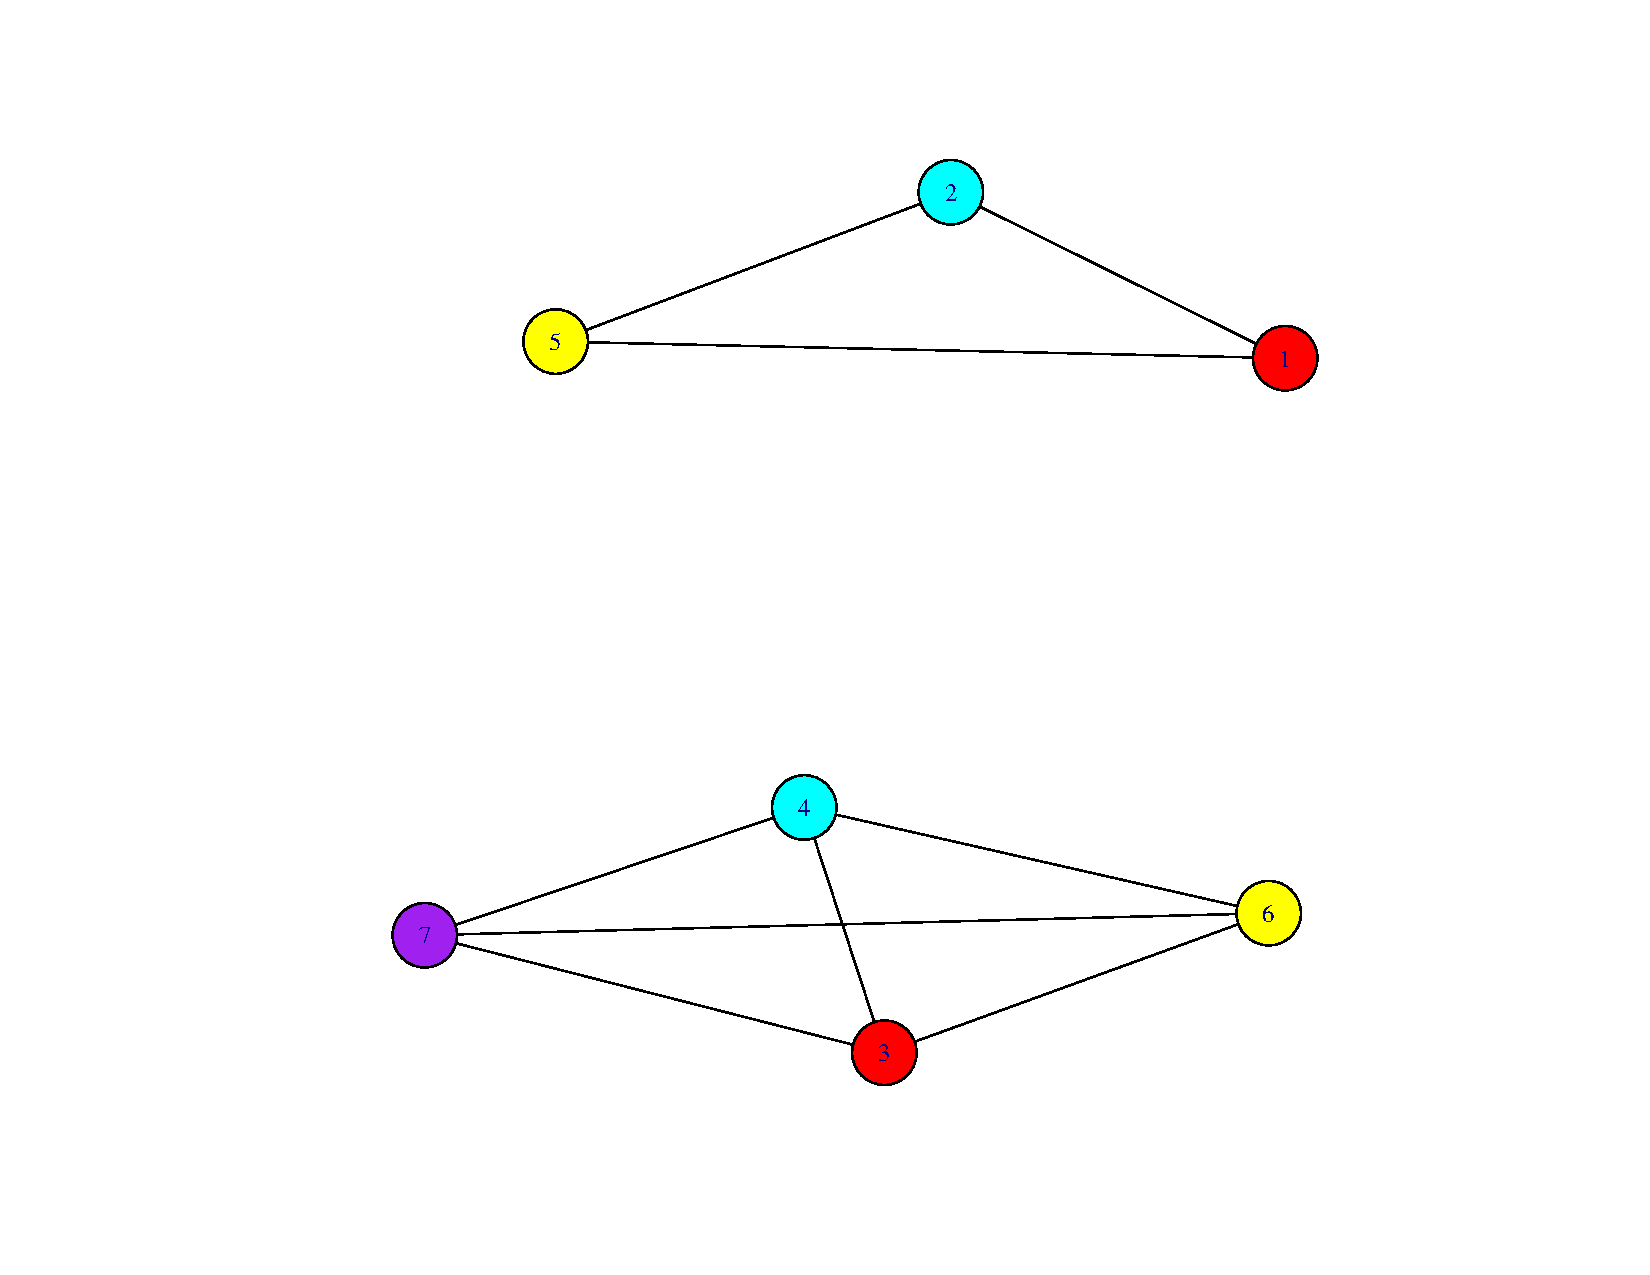
\includegraphics[scale=0.25]{img/v1M.pdf}
    \caption{Grafo M, coloração 1}
    \label{fig:v1M}
\end{figure}

Aplicando a versão 2 e 3 do algoritmo de coloração dos vértices, obtemos os seguintes resultados:

\begin{figure}[H]
    \centering
    \begin{minipage}{.5\textwidth}
      \centering
      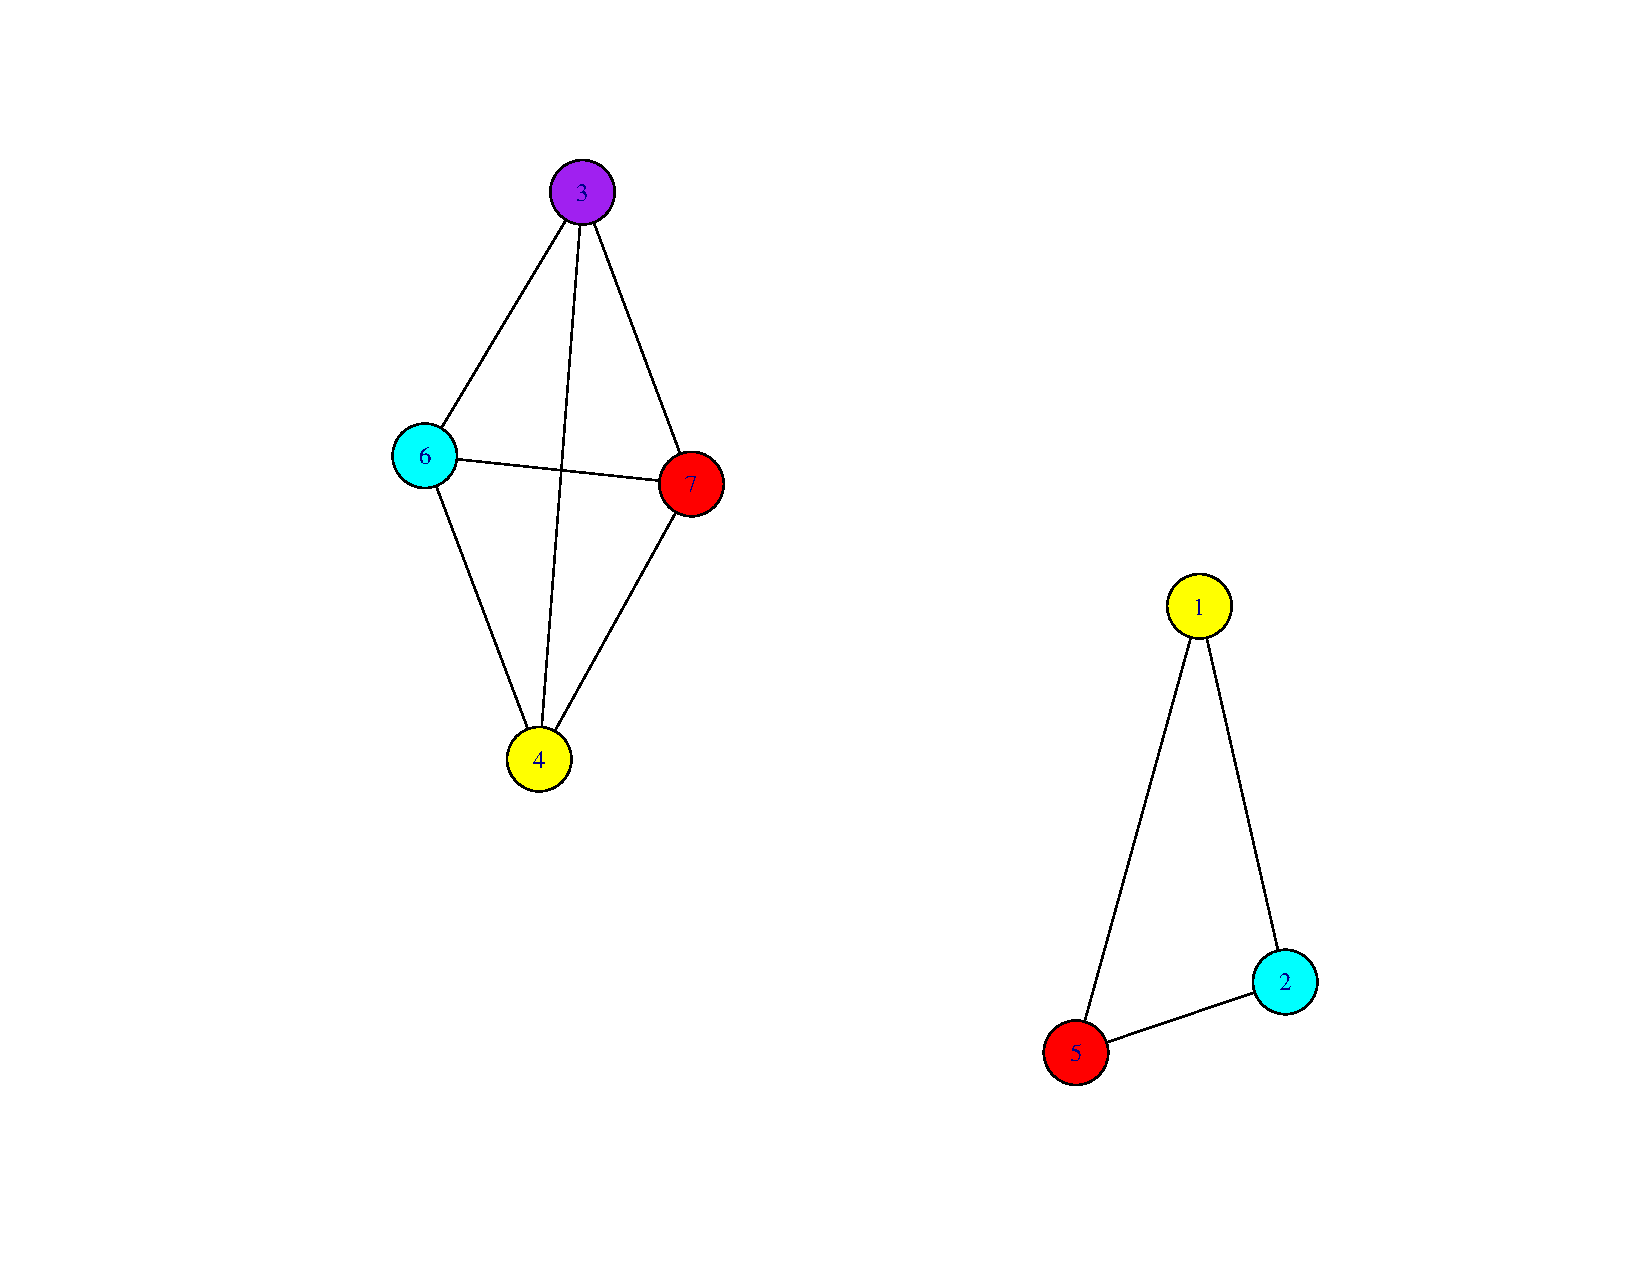
\includegraphics[scale=0.25]{img/v2M.pdf}
      \captionof{figure}{Grafo M, coloração 2}
      \label{fig:v2M}
    \end{minipage}%
    \begin{minipage}{.5\textwidth}
      \centering
      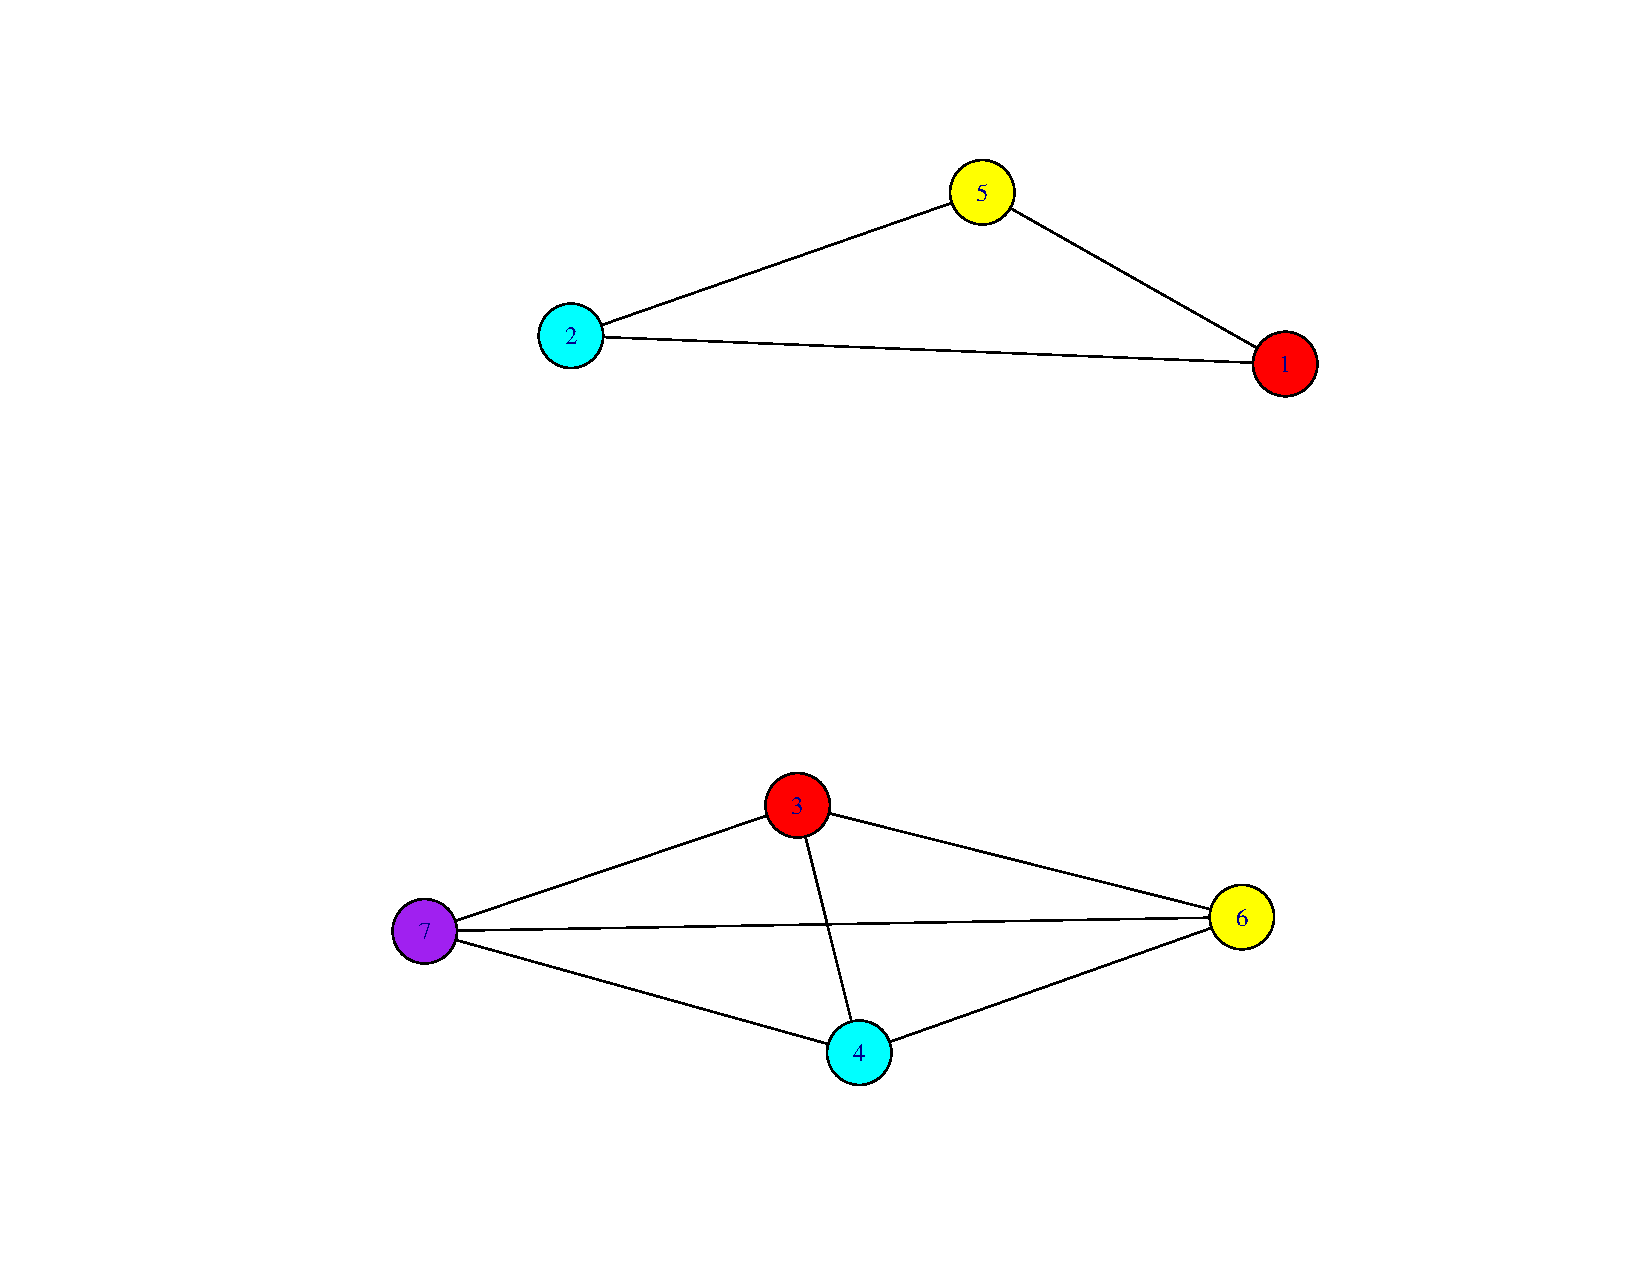
\includegraphics[scale=0.25]{img/v3M.pdf}
      \captionof{figure}{Grafo M, coloração 3}
      \label{fig:v3M}
    \end{minipage}
\end{figure}

Analisando os grafos obtidos, podemos ver que neste caso o algoritmo 1, 2 e 3 retornam colorações equivalentes.

\subsection*{Matriz $I$}

Seja $I$ a matriz 
$\begin{bmatrix}
    0&1&0&1&0&1\\
    1&0&1&0&0&1\\
    0&1&0&0&1&0\\
    1&0&0&0&1&0\\
    0&0&1&1&0&1\\
    1&1&0&0&1&0
\end{bmatrix}$. Aplicamos o algoritmo \textit{ColorizeVersion1.java} à matriz $I$.

A coloração obtida é a representada no seguinte grafo:

\begin{figure}[H]
    \centering
        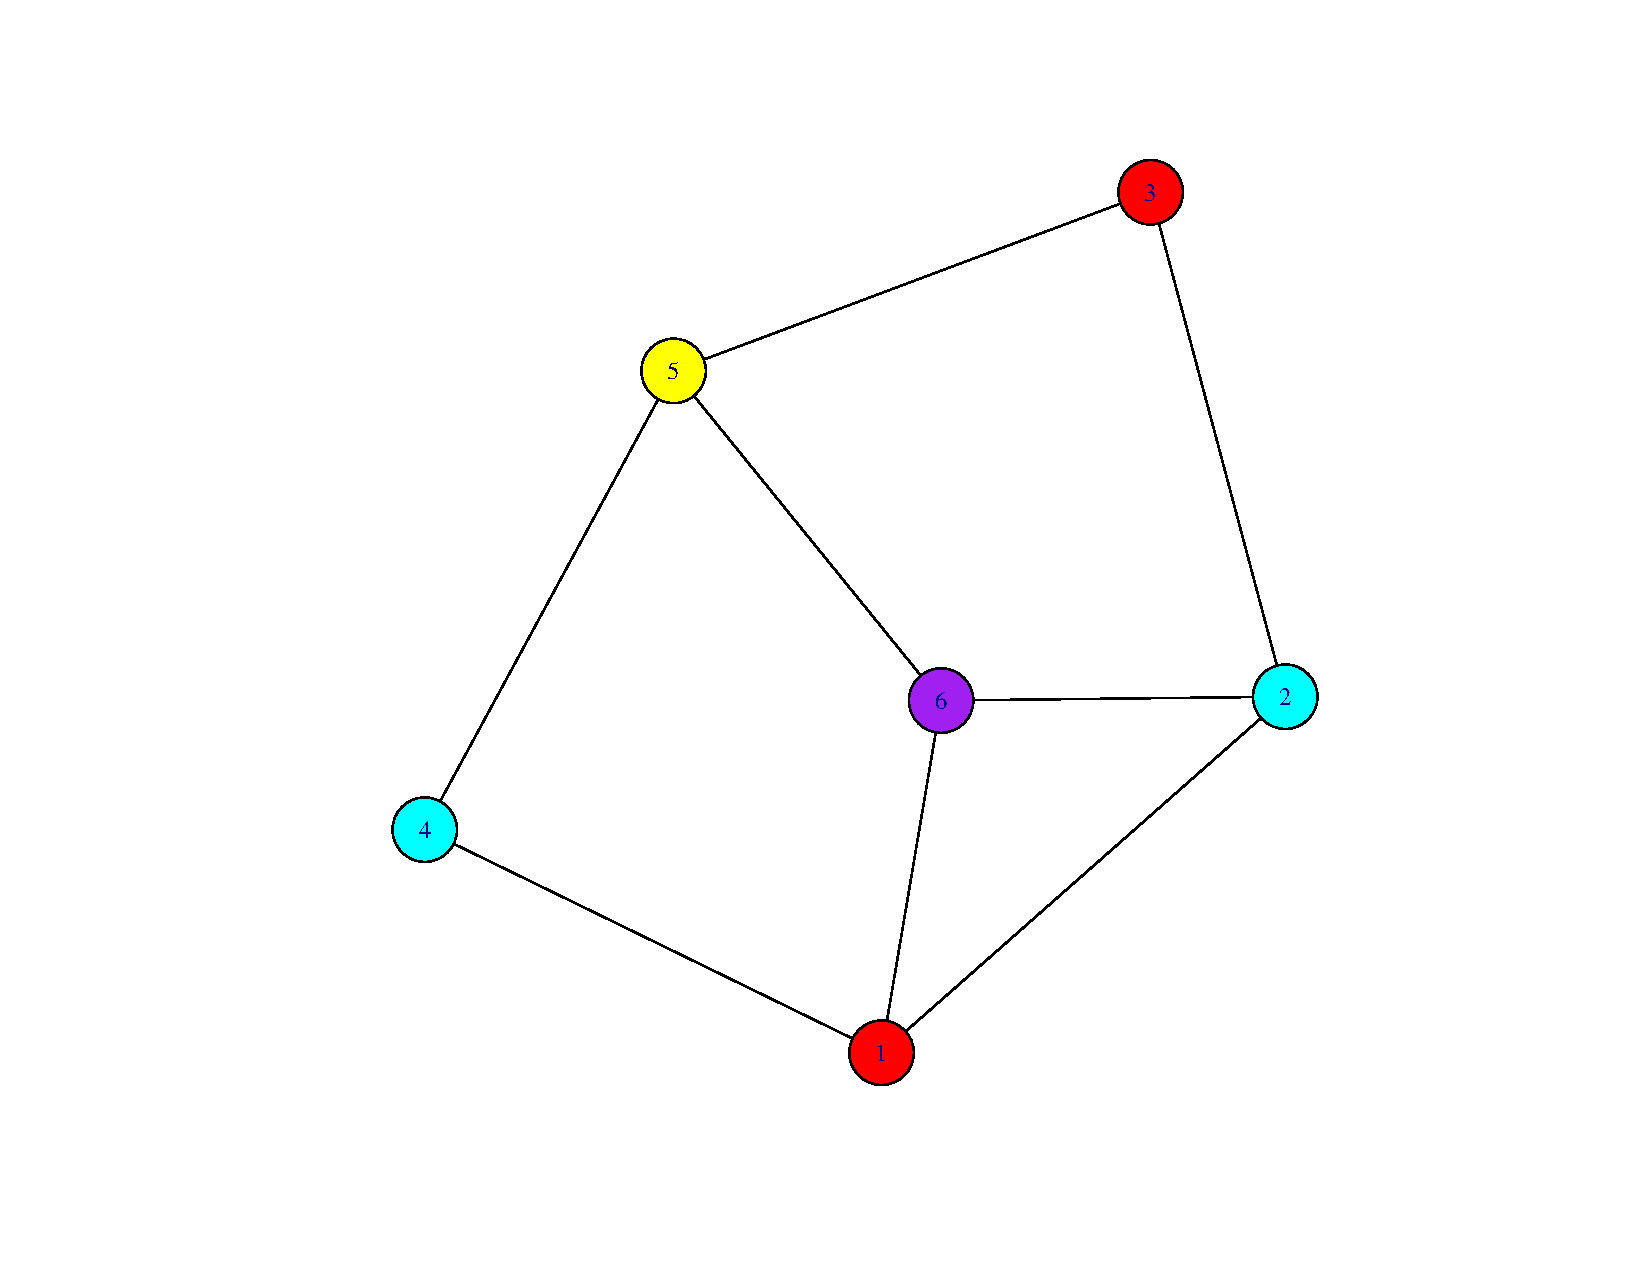
\includegraphics[scale=0.25]{img/v1I.pdf}
    \caption{Grafo I, coloração 1}
    \label{fig:v1I}
\end{figure}

Aplicando a versão 2 e 3 do algoritmo de coloração dos vértices, obtemos os seguintes resultados:

\begin{figure}[H]
    \centering
    \begin{minipage}{.5\textwidth}
      \centering
      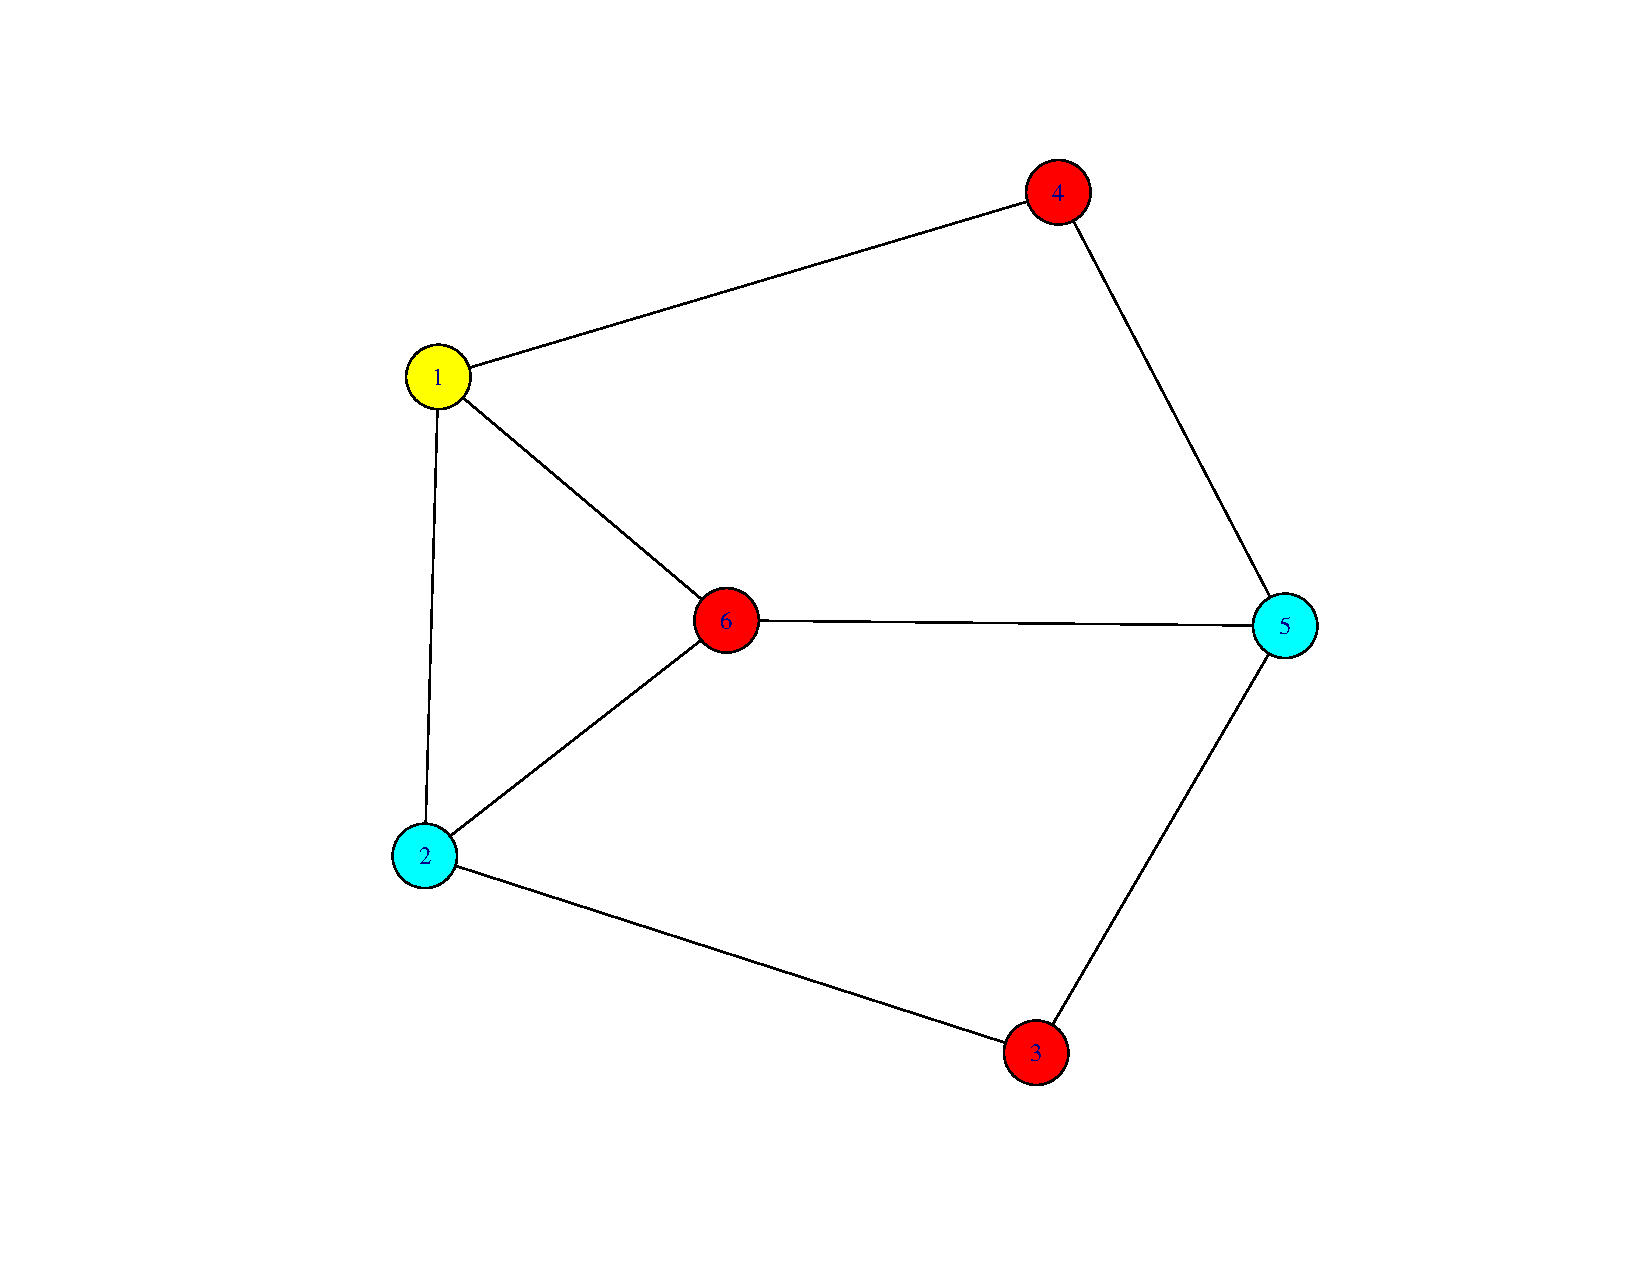
\includegraphics[scale=0.25]{img/v2I.pdf}
      \captionof{figure}{Grafo I, coloração 2}
      \label{fig:v2I}
    \end{minipage}%
    \begin{minipage}{.5\textwidth}
      \centering
      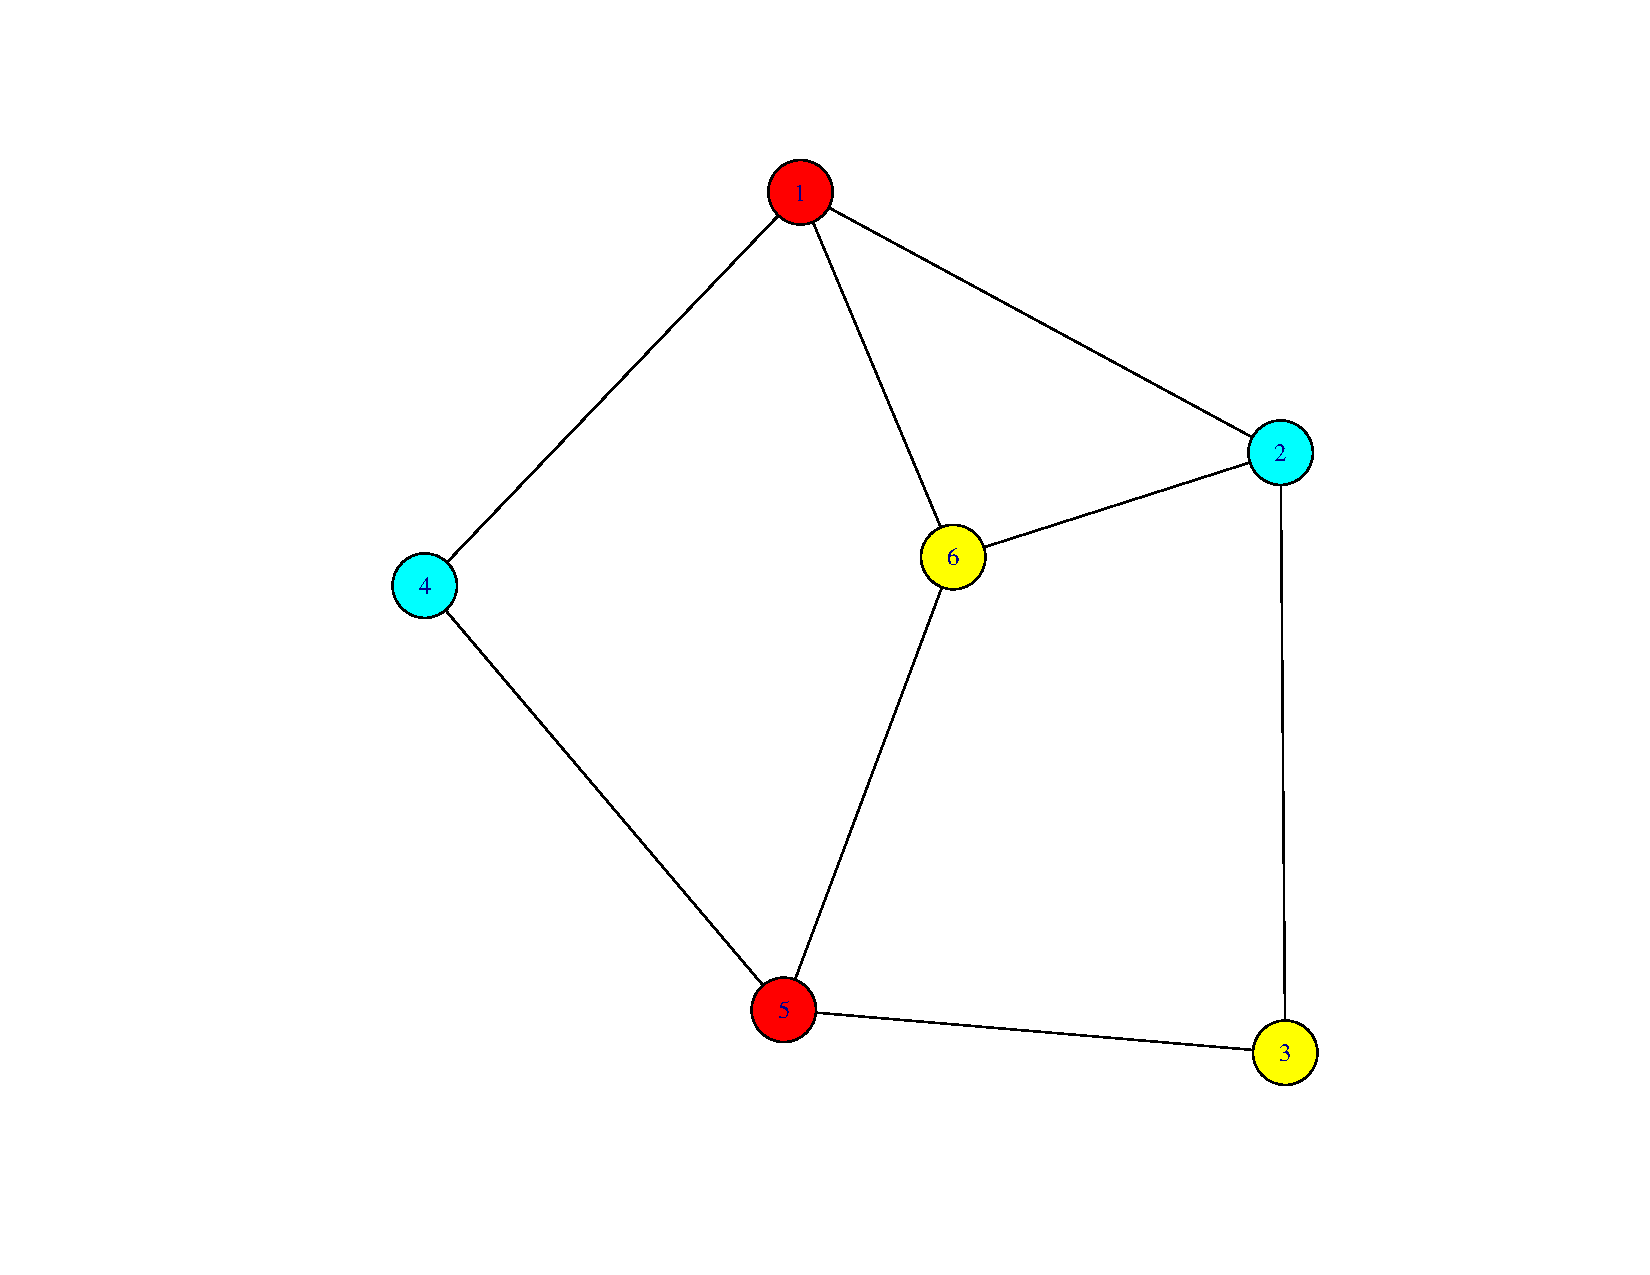
\includegraphics[scale=0.25]{img/v3I.pdf}
      \captionof{figure}{Grafo I, coloração 3}
      \label{fig:v3I}
    \end{minipage}
\end{figure}

Analisando os grafos obtidos, podemos ver que neste caso o algoritmo 1 não consegue encontrar uma coloração mínima, ao contrário do que acontece com as versões 2 e 3.

Vamos agora analisar se a versão 3 consegue obter uma coloração mais baixa em algum caso, relativamente à versão 2.

\subsection*{Matriz $F$}

Seja $F$ a matriz 
$\begin{bmatrix}
    0&1&1&1&1&0&1&1&1&1\\
    1&0&1&1&1&0&0&1&0&1\\
    1&1&0&1&1&1&1&1&1&1\\
    1&1&1&0&1&1&0&0&1&1\\
    1&1&1&1&0&1&1&0&0&0\\
    0&0&1&1&1&0&1&1&1&0\\
    1&0&1&0&1&1&0&1&0&1\\
    1&1&1&0&0&1&1&0&1&1\\
    1&0&1&1&0&1&0&1&0&1\\
    1&1&1&1&0&0&1&1&1&0
\end{bmatrix}$. Aplicamos o algoritmo \textit{ColorizeVersion2.java} à matriz $F$.

A coloração obtida é a representada no seguinte grafo:

\begin{figure}[H]
    \centering
        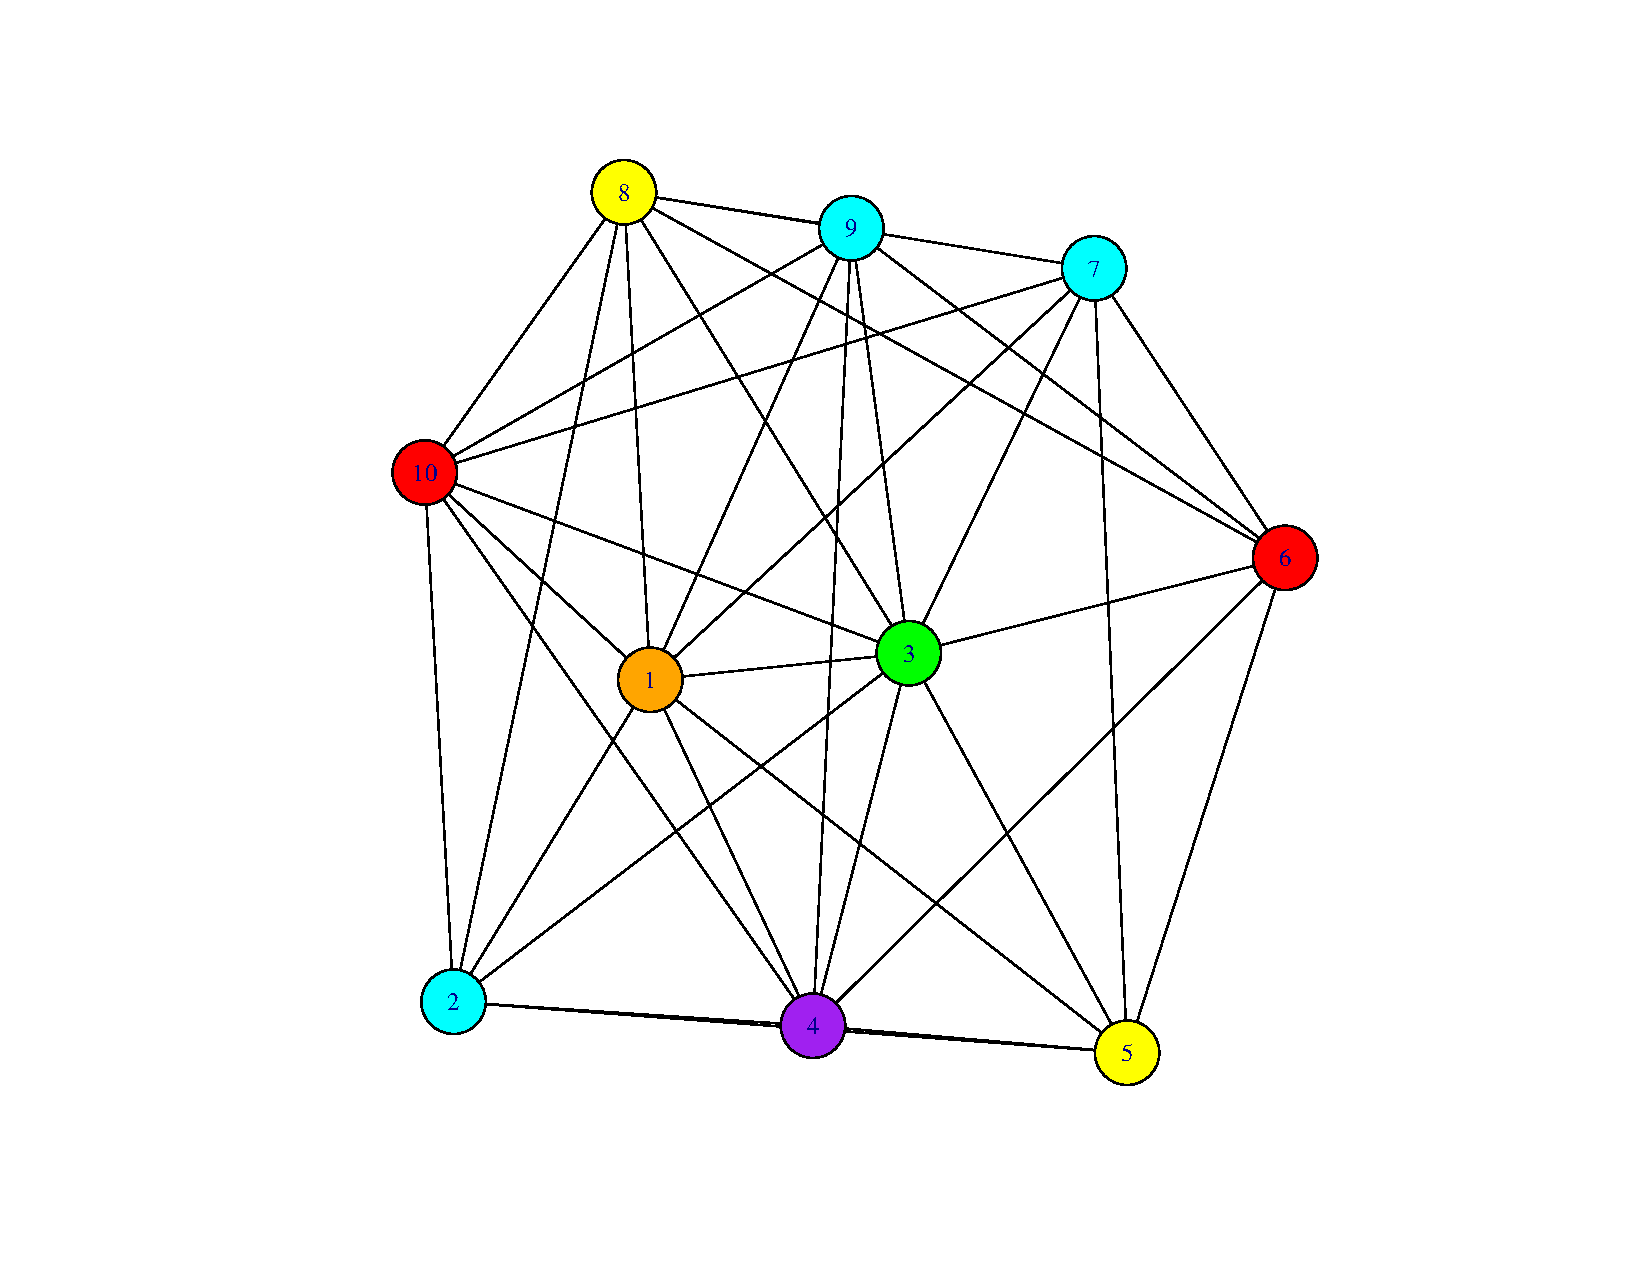
\includegraphics[scale=0.25]{img/v2F.pdf}
    \caption{Grafo F, coloração 2}
    \label{fig:v2F}
\end{figure}

Aplicando a versão 1 e 3 do algoritmo de coloração dos vértices, obtemos os seguintes resultados:

\begin{figure}[H]
    \centering
    \begin{minipage}{.5\textwidth}
      \centering
      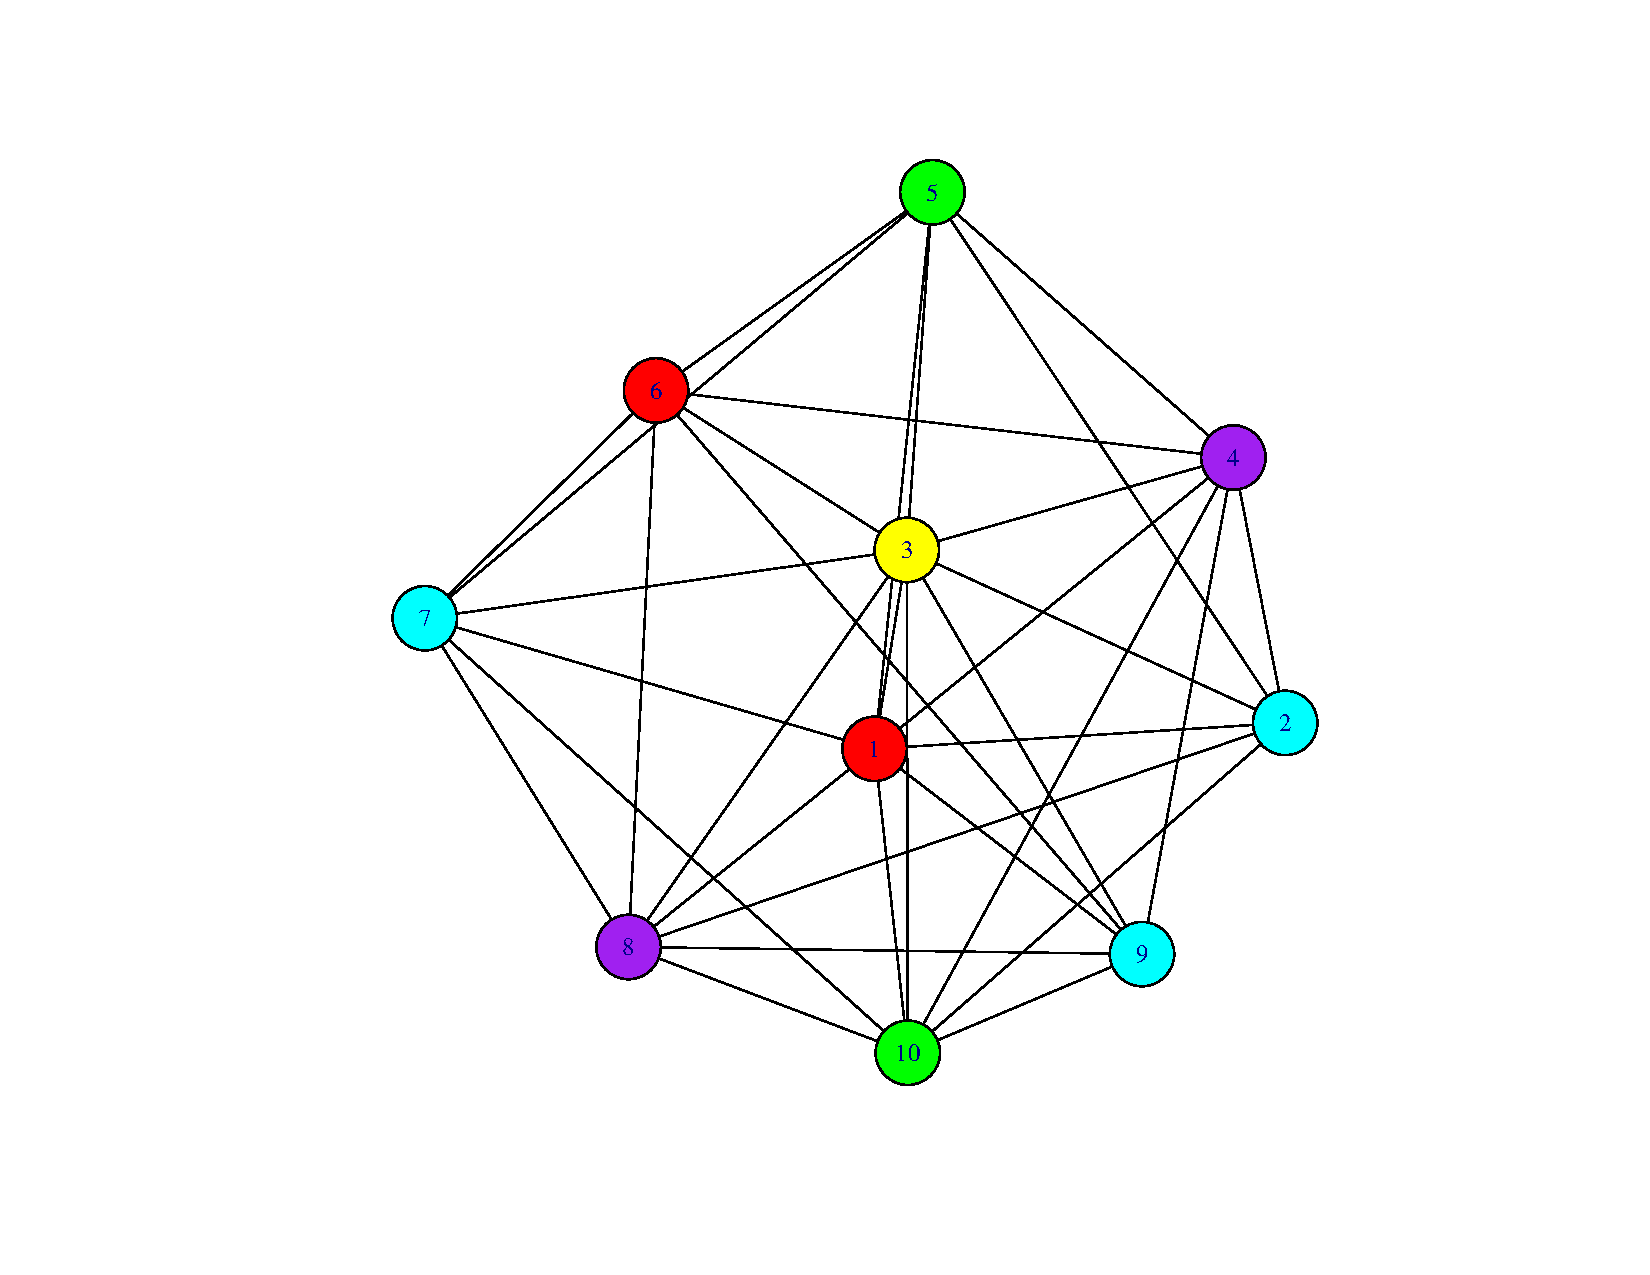
\includegraphics[scale=0.25]{img/v1F.pdf}
      \captionof{figure}{Grafo F, coloração 1}
      \label{fig:v1F}
    \end{minipage}%
    \begin{minipage}{.5\textwidth}
      \centering
      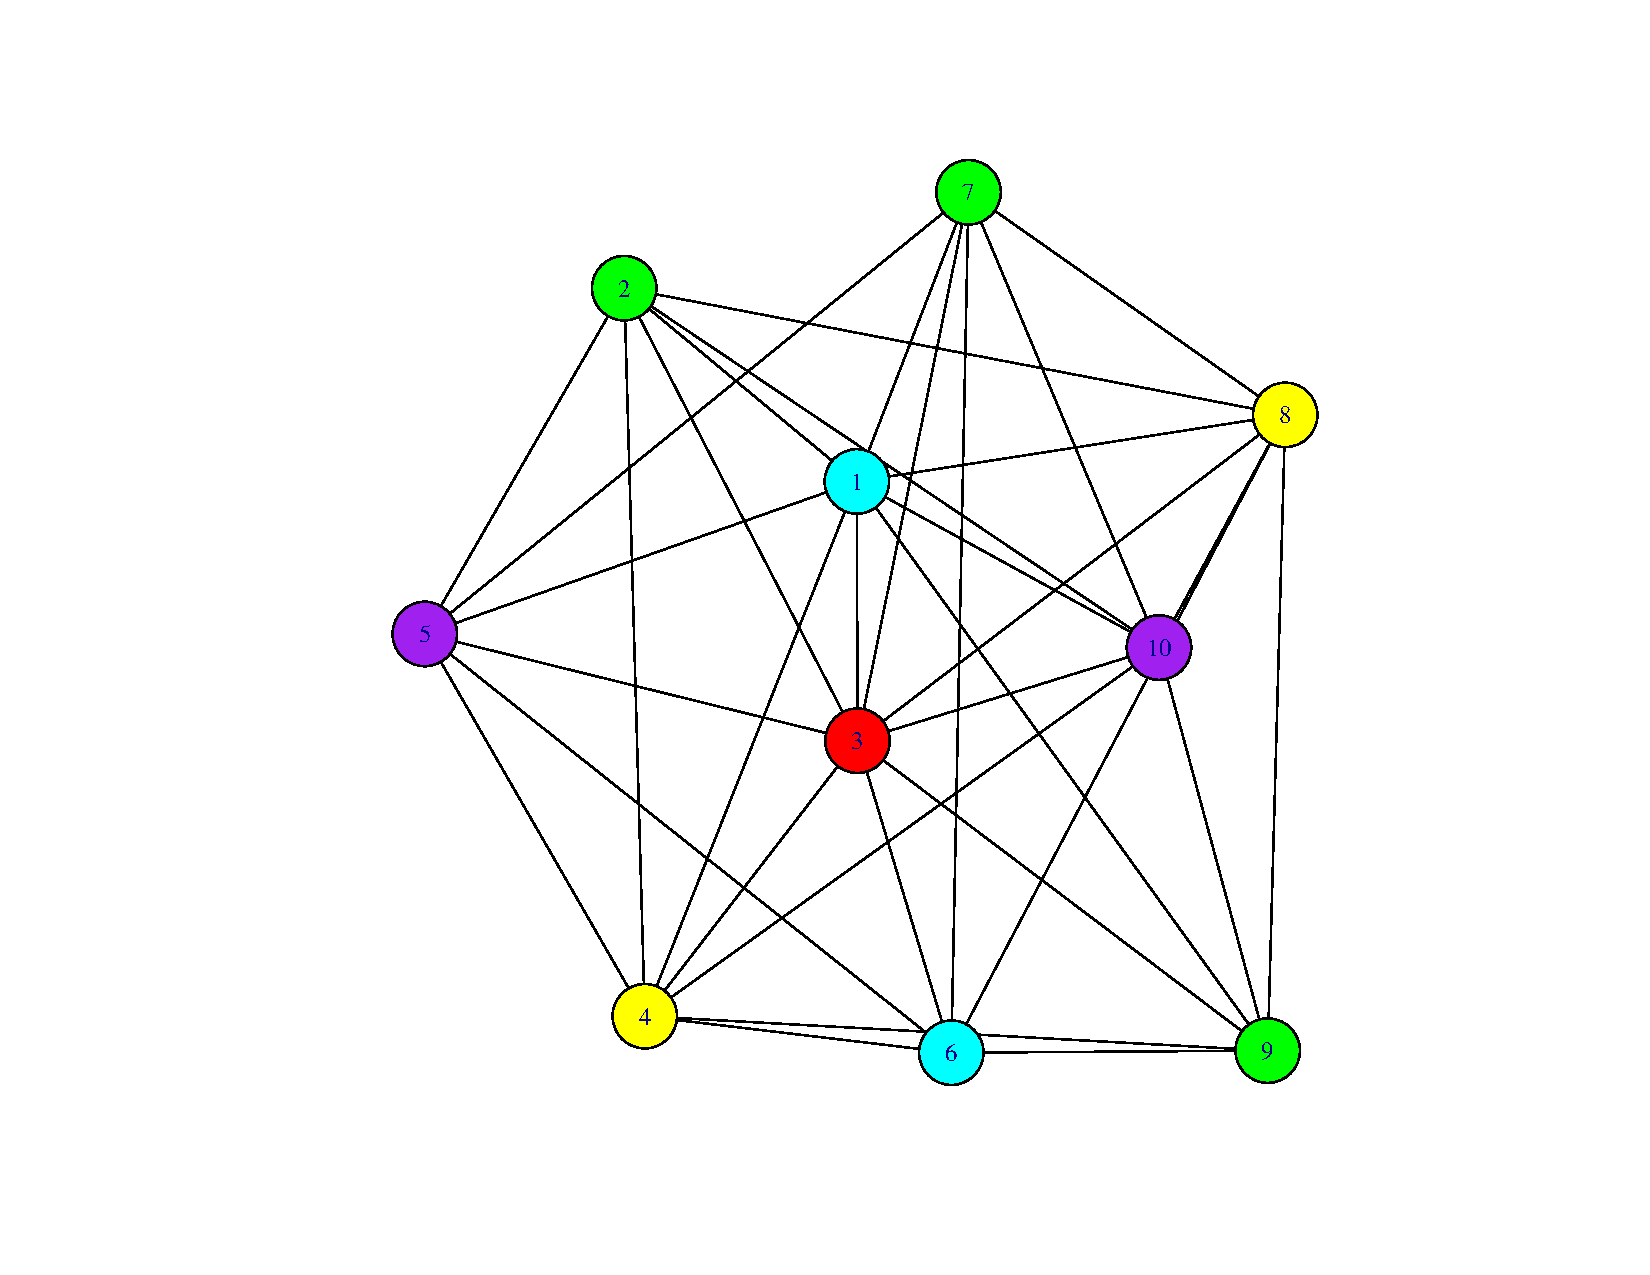
\includegraphics[scale=0.25]{img/v3F.pdf}
      \captionof{figure}{Grafo F, coloração 3}
      \label{fig:v3F}
    \end{minipage}
\end{figure}

Analisando os grafos obtidos, podemos ver que neste caso o algoritmo 2 não consegue encontrar uma coloração mínima, ao contrário do que acontece com as versões 1 e 3.

\section{Exercício 2}

O algoritmo implementado é o representado em \ref{fig:dfsAl}.

Para dar resposta à alínea b) foi utilizado o método \textit{haveNonVisitedVertexes ()} para verificar se na lista de vértices do grafo existe algum vértice não visitado. 

O algoritmo só termina quando não existirem mais vértices não visitados: \textit{while (dfs.haveNonVisitedVertexes())}.

Para a alínea c) foi introduzida um verficação antes de marcar um vértice como visitado. A condição \textit{(!dfs.getVisited(n) \&\& !dfs.haveNonVisitedPredecessors(n))} verifica se o vértice em questão já foi visitado e se contém algum predecessor não visitado.

Nos grafos apresentados nesta secção, o número em cada vértice representa a ordem pela qual o vértice foi visitado.

\subsection*{Matriz $P$}

Para o caso da matriz $P$ = $\begin{bmatrix}
    0&1&0&0&0\\
    0&0&1&0&0\\
    0&0&0&1&0\\
    0&0&0&0&1\\
    0&0&0&0&0
\end{bmatrix}$, o resultado obtido é:
\begin{figure}[H]
    \centering
        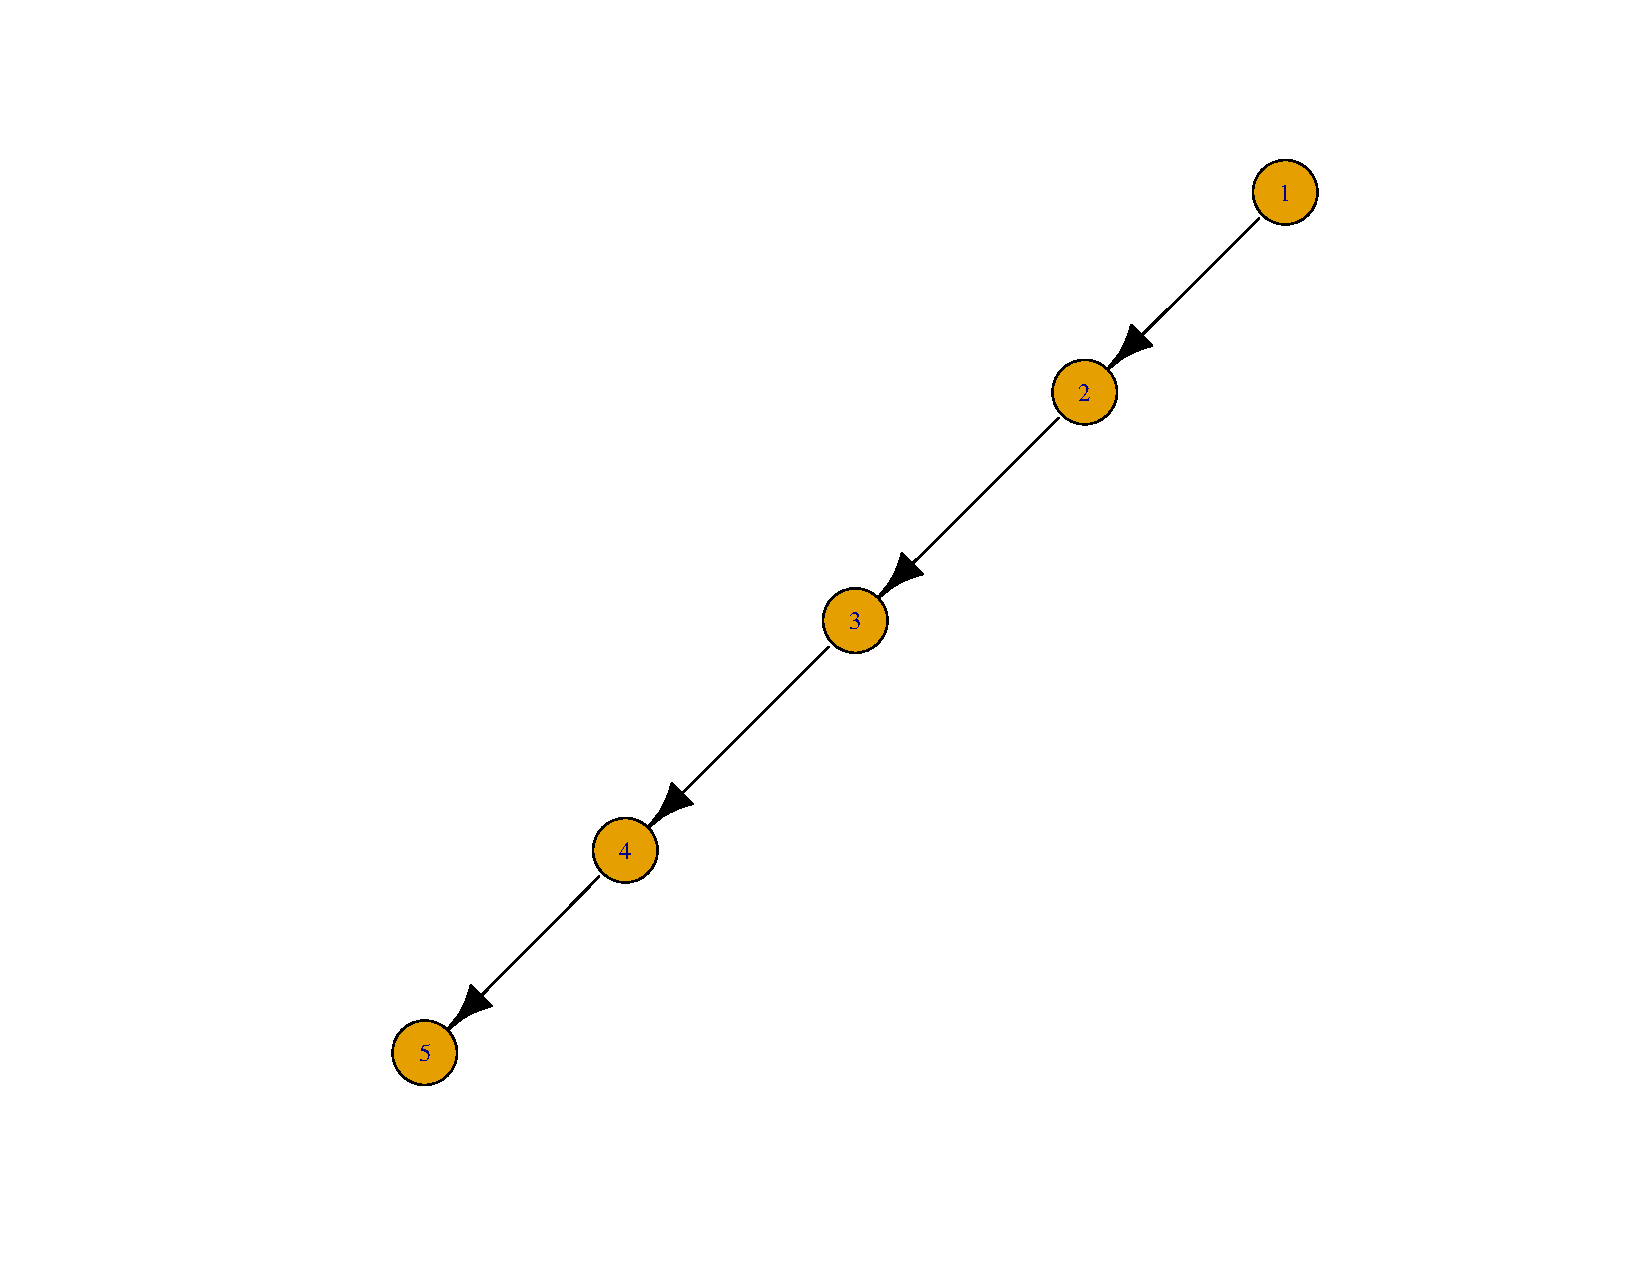
\includegraphics[scale=0.25]{img/dfsP.pdf}
    \caption{Grafo P, pesquisa em profundidade}
    \label{fig:dfsP}
\end{figure}

Neste caso podemos ver que os vértices são visitados de forma sequêncial (como era previsto), ou seja, analisando valor de cada vértice podemos ver que é sempre superior ao seu antecessor.

\subsection*{Matriz $O$}

Para o caso da matriz $O$ = $\begin{bmatrix}
    0&1&1\\
    0&0&-1\\
    0&0&0
\end{bmatrix}$, o resultado obtido é:
\begin{figure}[H]
    \centering
        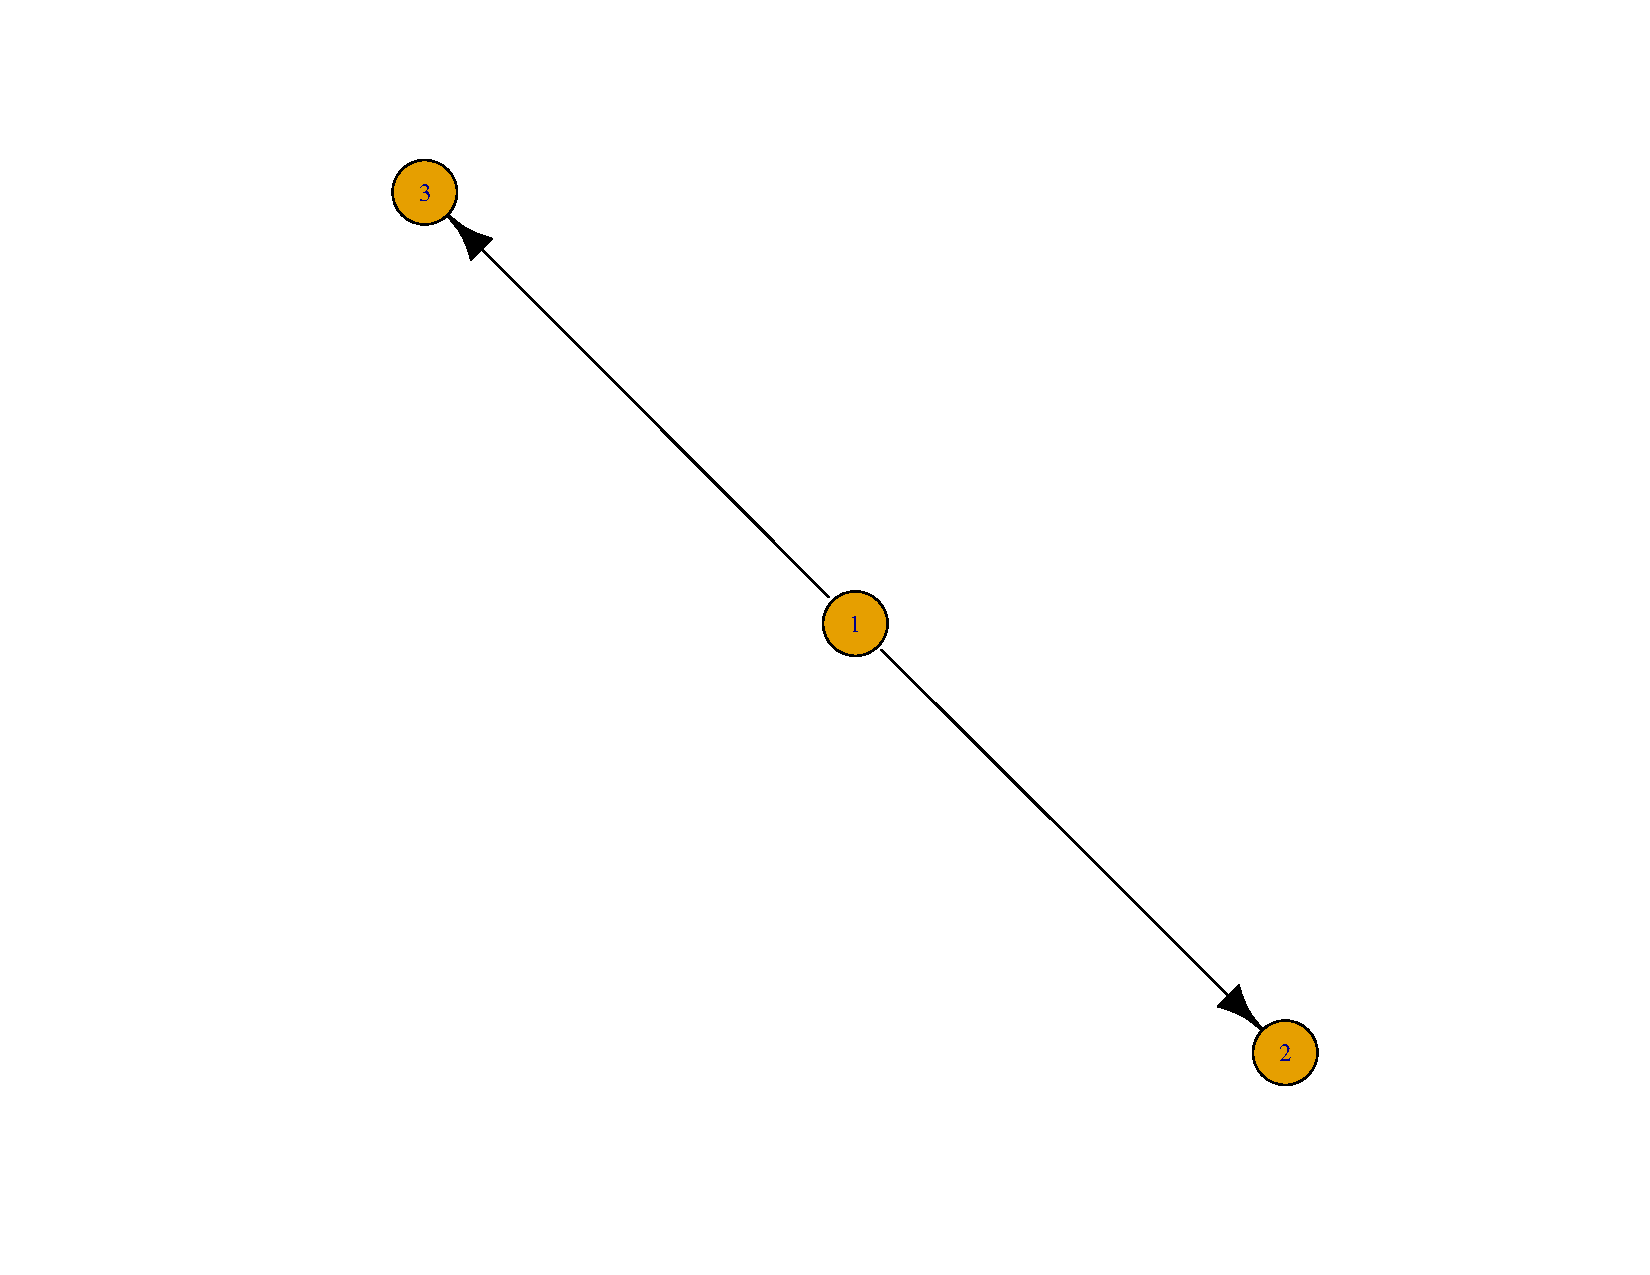
\includegraphics[scale=0.25]{img/dfsO.pdf}
    \caption{Grafo O, pesquisa em profundidade}
    \label{fig:dfsP}
\end{figure}

À semelhança do exemplo anterior podemos ver que os vértices contém sempre um número superior ao seu antecessor.

\subsection*{Matriz $A$}

Para o caso da matriz $A$=$\begin{bmatrix}
    0&1&1&0&0&0&0\\
    -1&0&0&1&1&0&0\\
    -1&0&0&0&0&1&0\\
    0&-1&0&0&0&0&1\\
    0&-1&0&0&0&-1&1\\
    0&0&-1&0&1&0&1\\
    0&0&0&-1&-1&-1&0
\end{bmatrix}$, o resultado obtido é:
\begin{figure}[H]
    \centering
        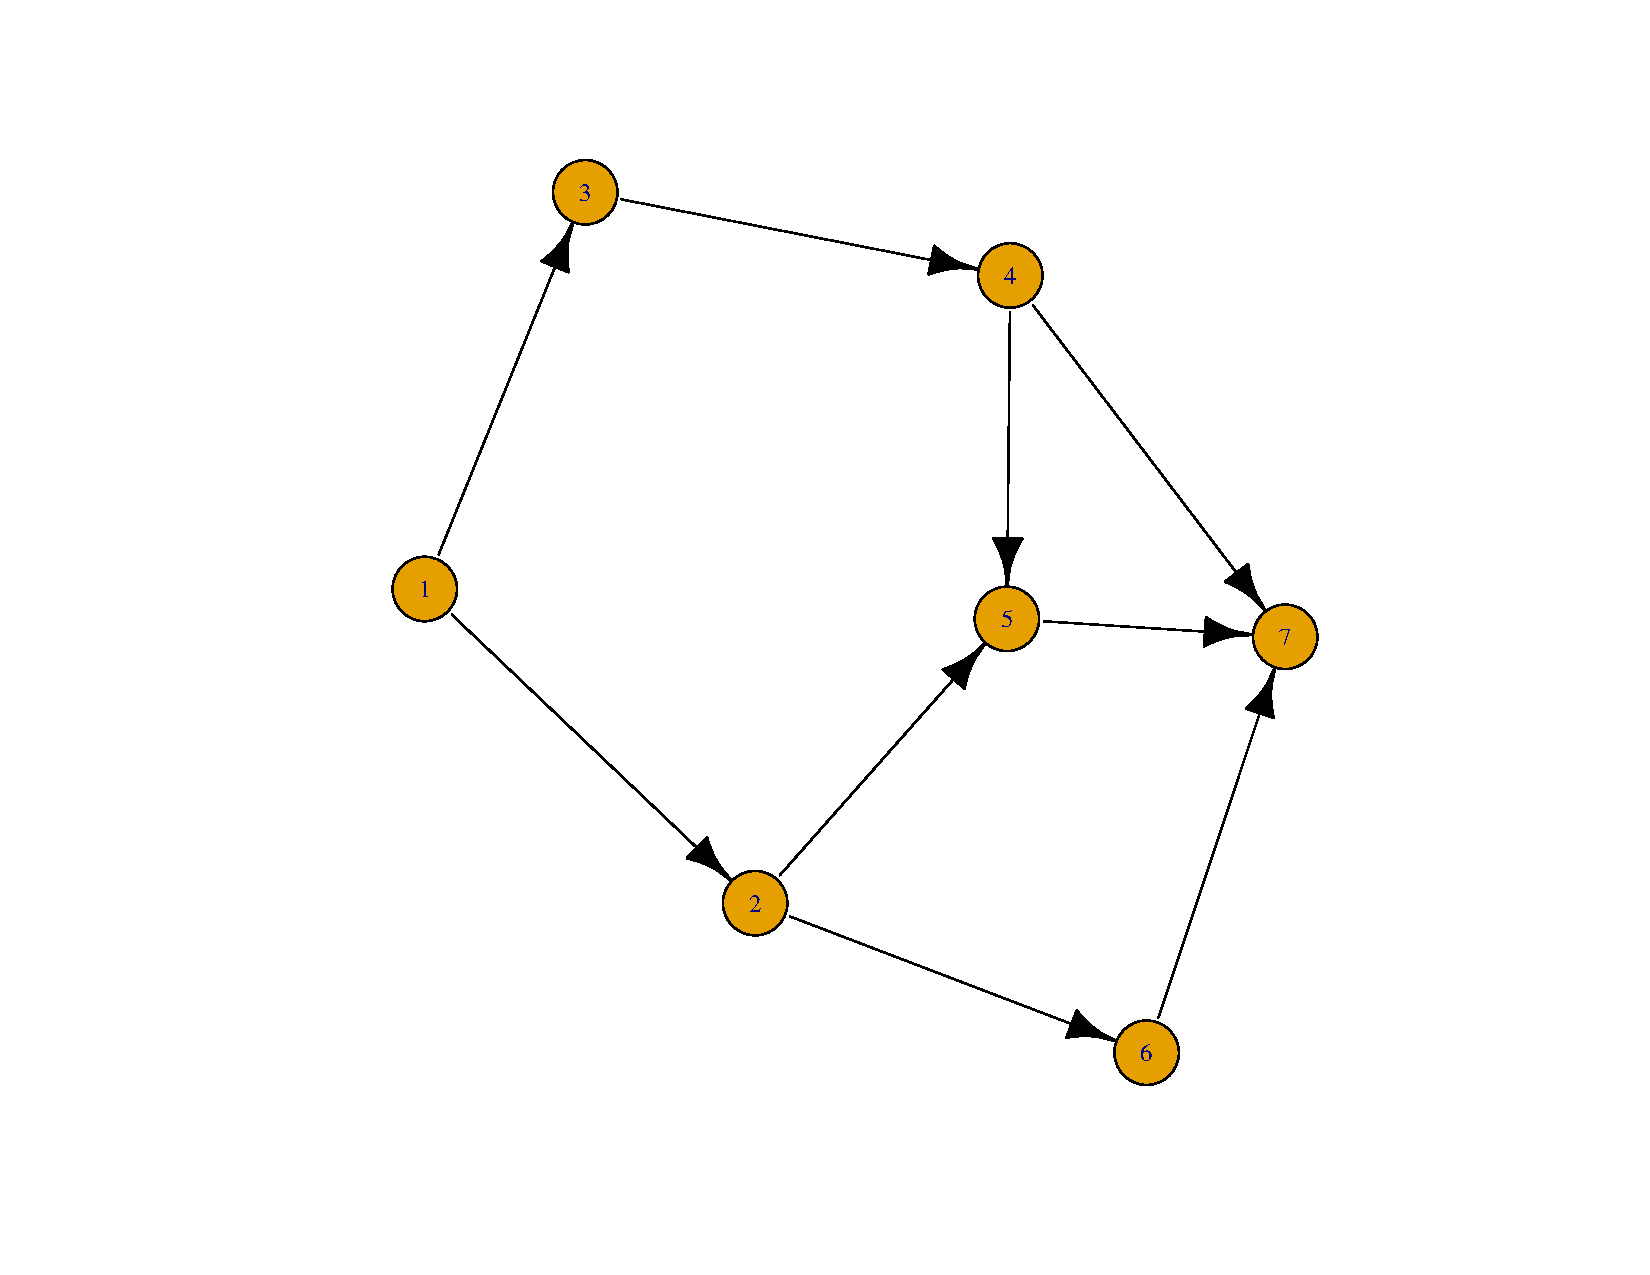
\includegraphics[scale=0.25]{img/dfsA.pdf}
    \caption{Grafo A, pesquisa em profundidade}
    \label{fig:dfsP}
\end{figure}

Sendo este um caso mais complexo quando comparado com os exemplos anteriores podemos continuar a concluir que os vértices são sempre visitados após os seus antecessores.

\subsection*{Matriz $Q$}

Para o caso da matriz $Q$ = $\begin{bmatrix}
    0&1&0&0&0&0&0\\
    0&0&1&0&0&0&0\\
    0&0&0&1&0&0&0\\
    0&0&0&0&0&0&0\\
    0&0&0&0&0&1&0\\
    0&0&0&0&0&0&1\\
    0&0&0&0&0&0&0
\end{bmatrix}$, o resultado obtido é:
\begin{figure}[H]
    \centering
        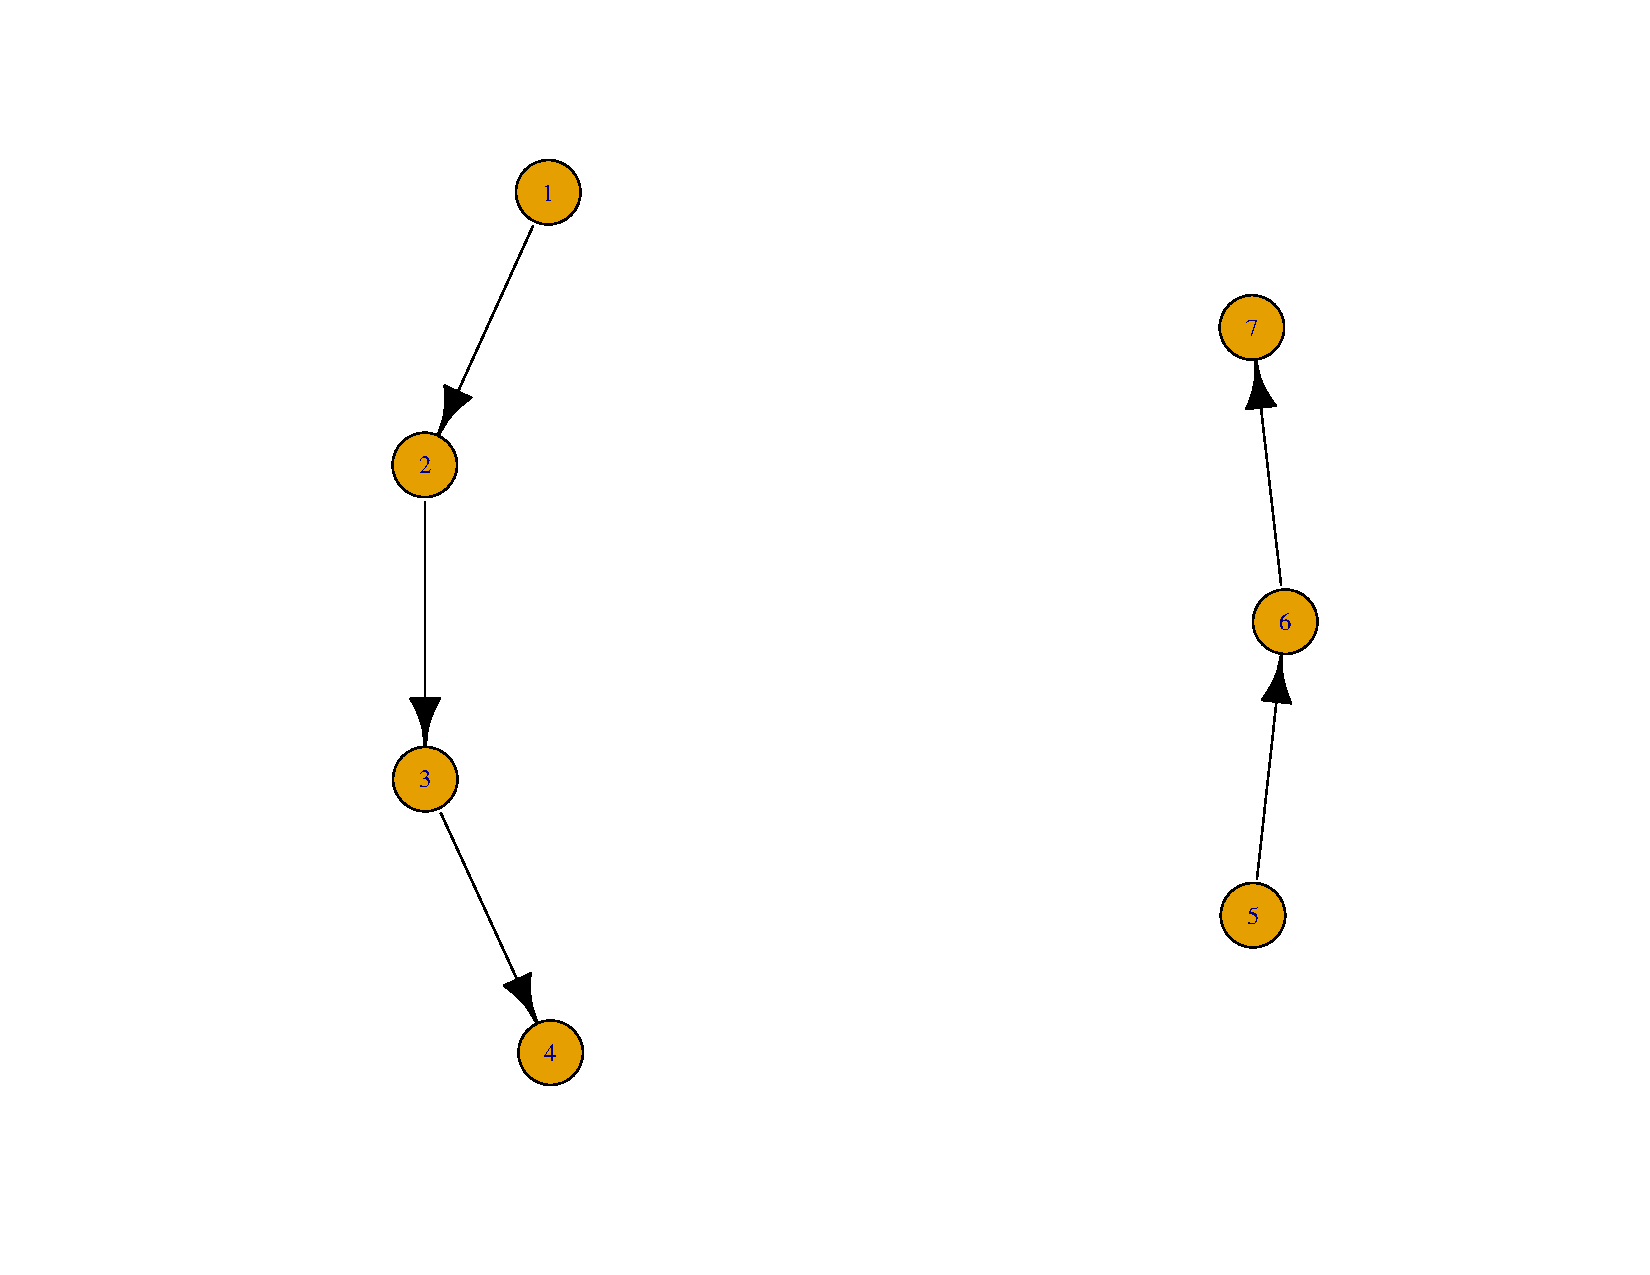
\includegraphics[scale=0.25]{img/dfsQ.pdf}
    \caption{Grafo Q, pesquisa em profundidade}
    \label{fig:dfsP}
\end{figure}

Neste caso temos um grafo não conexo, contudo todos os vértices contém uma ordem pela qual foram visitados. Daqui podemos concluir que o algoritmo visita todos os vértices do grafo, sendo ele conexo ou não.

\subsection*{Matriz $M25$}

Para o caso da matriz $M25$, o resultado obtido é:
\begin{figure}[H]
    \centering
        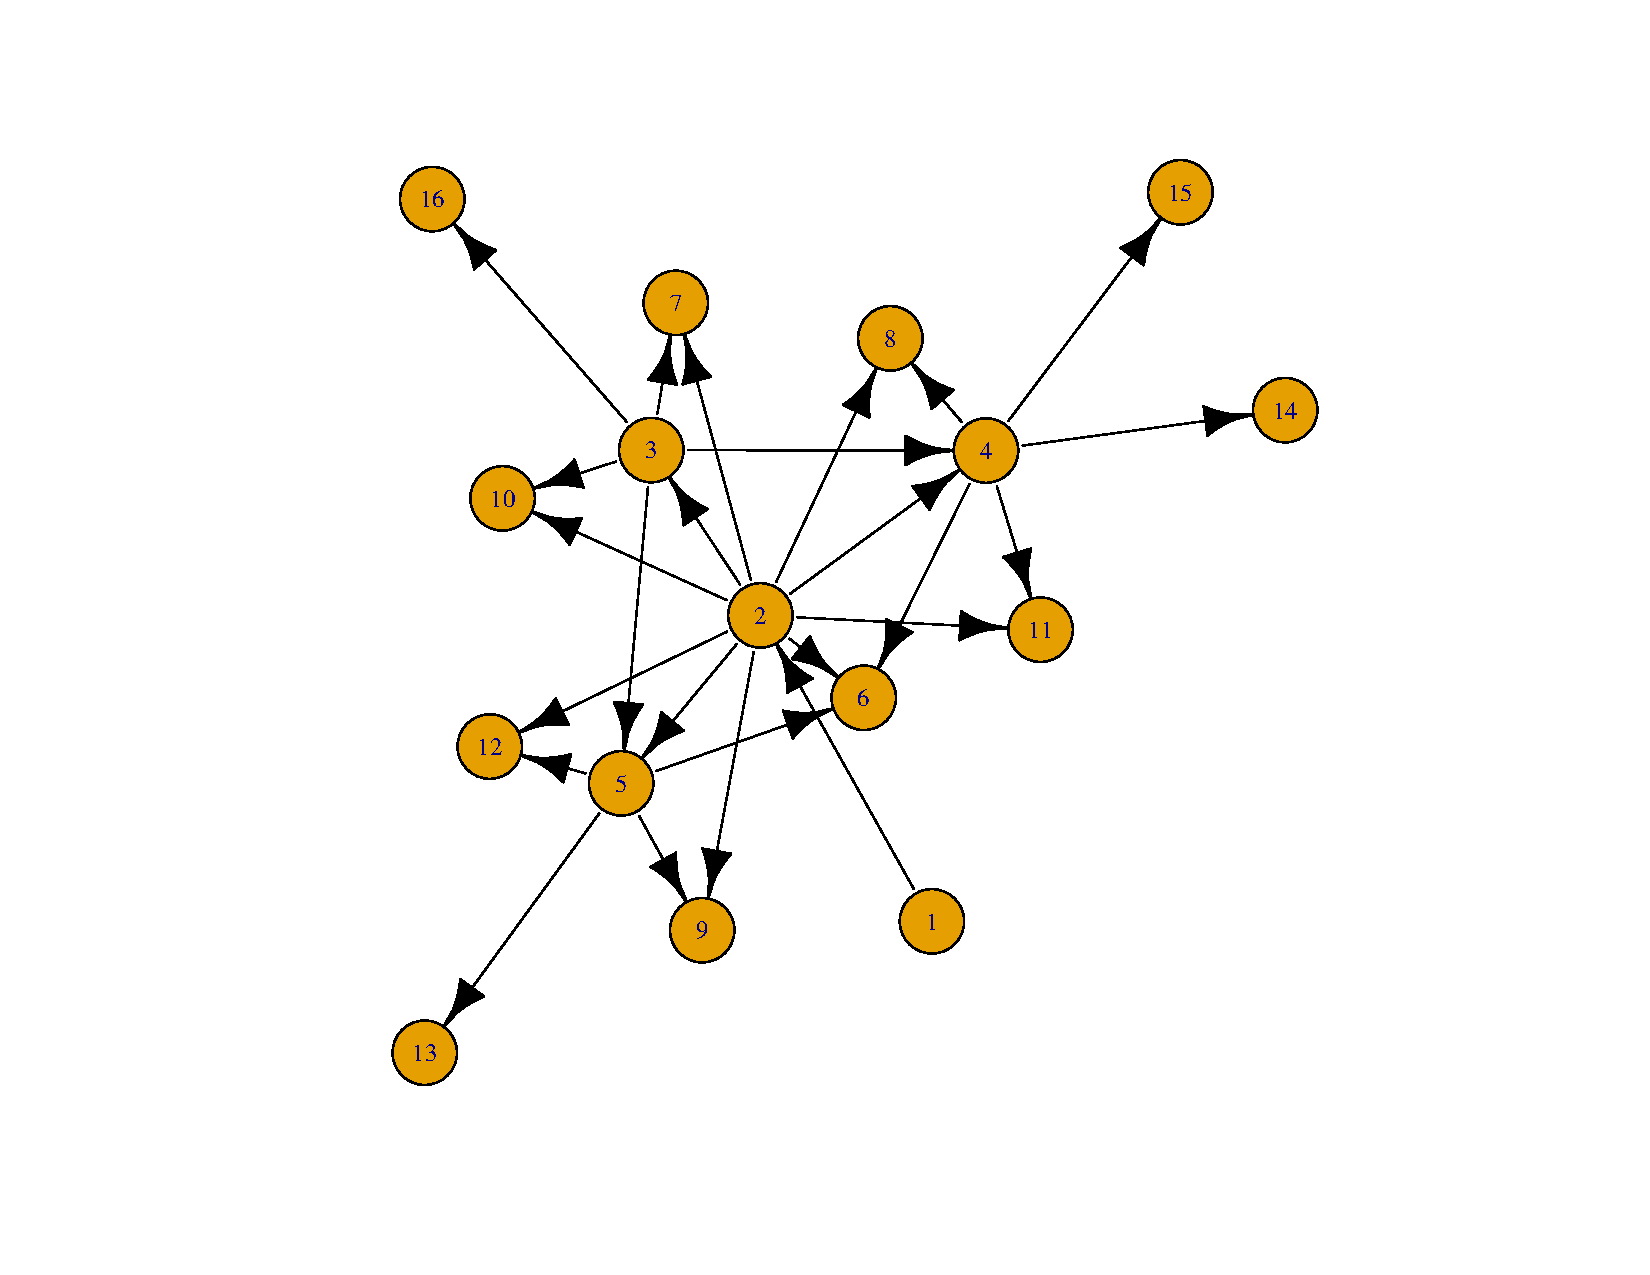
\includegraphics[scale=0.25]{img/dfsM25.pdf}
    \caption{Grafo M25, pesquisa em profundidade}
    \label{fig:dfsP}
\end{figure}

Apresento a baixo a lista dos vértices juntamente com a ordem pela qual foram visitados, de forma a poder visualizar melhor o resultado obtido uma vez que o grafo é mais complexo.

\begin{lstlisting}
 1  [1]      2 [2]      3 [3]      4 [4]      5 [5]      10 [6]
11  [7]     12 [8]     13 [9]     14 [10]    15 [11]     16 [12]
 9  [13]     7 [14]     8 [15]     6 [16]
\end{lstlisting}

sendo o primeiro valor o \textit(id) do vértice e o segundo a ordem pela qual foi visitado (a lista está ordenada pela ordem cresente da visita dos vértices).

Analisando o ficheiro \textit{log\_dfs.txt} (em anexo) conseguimos ver o procedimento feito pelo algoritmo.

\subsection*{Matriz $M50$}

Para o caso da matriz $M50$, o resultado obtido é:
\begin{figure}[H]
    \centering
        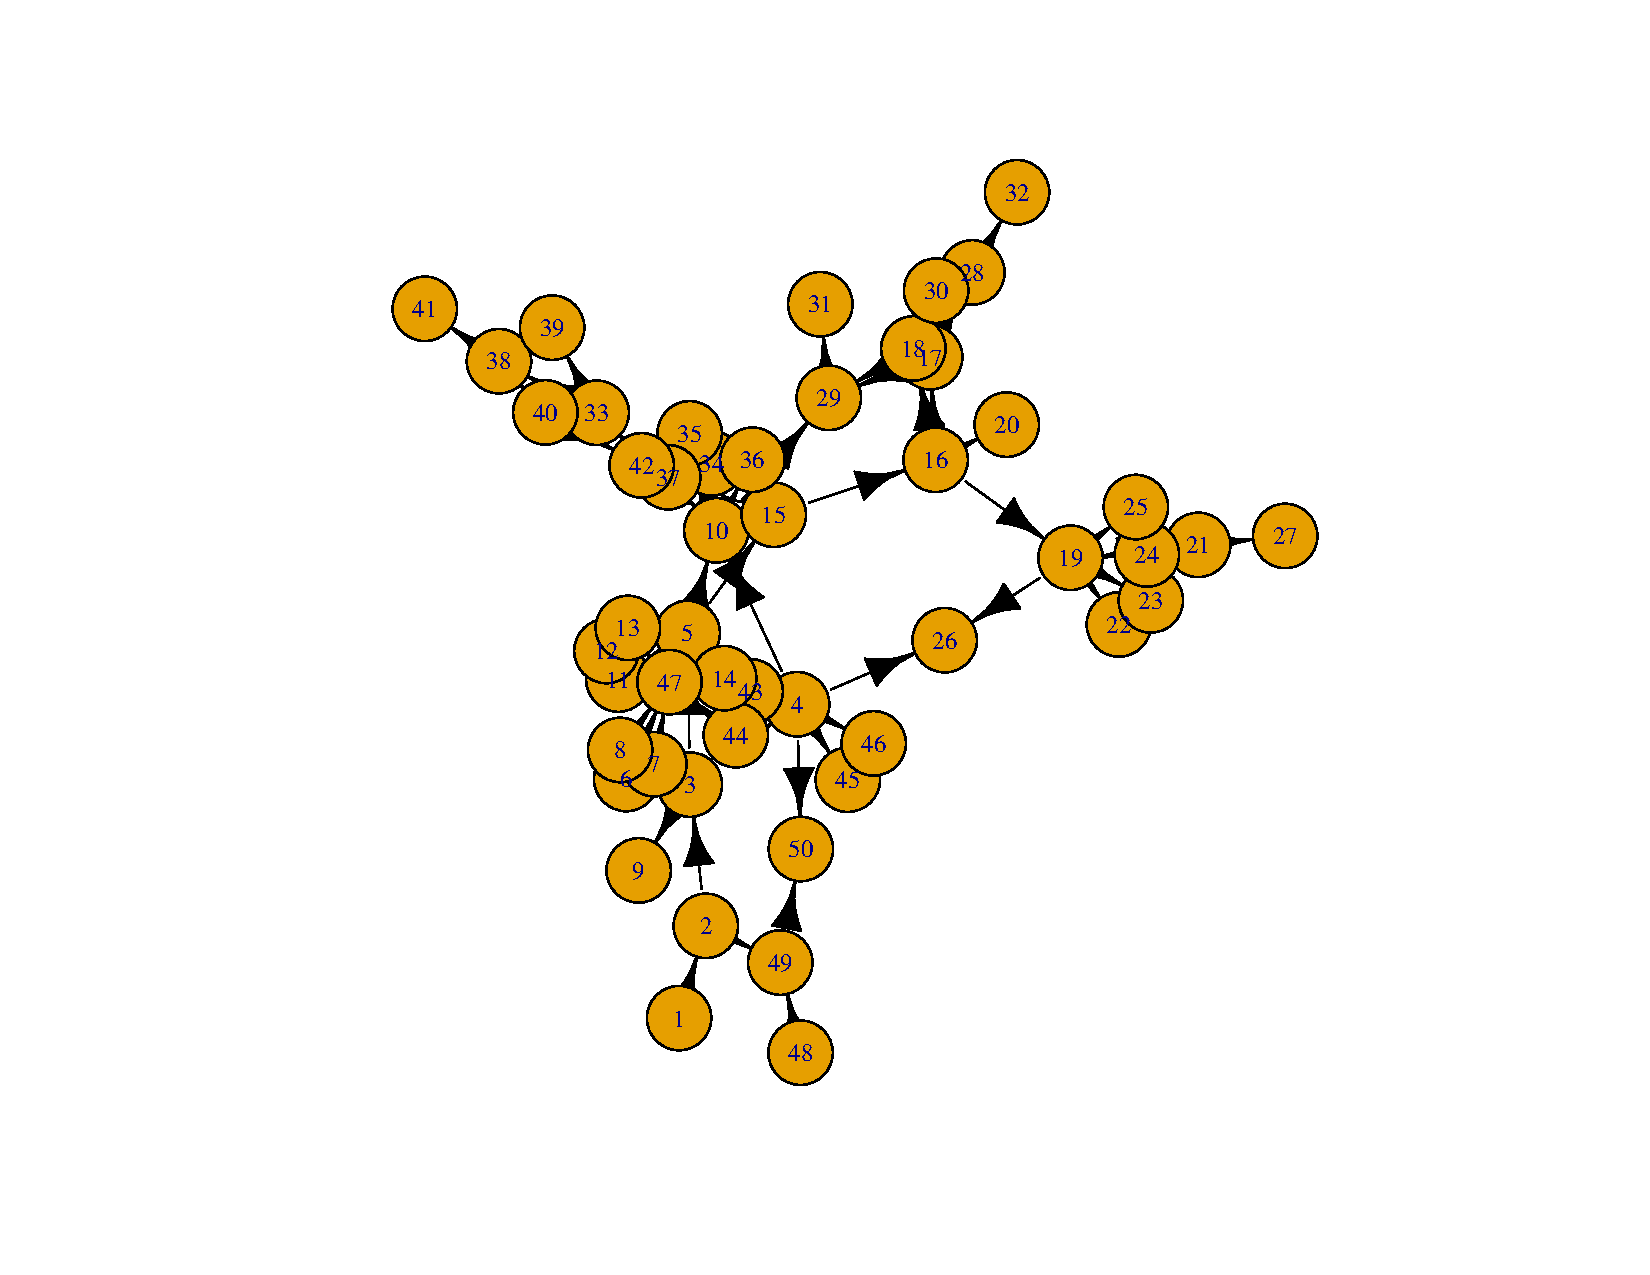
\includegraphics[scale=0.25]{img/dfsM50.pdf}
    \caption{Grafo M50, pesquisa em profundidade}
    \label{fig:dfsP}
\end{figure}

À semelhança do exemplo anterior, apresento a baixo a lista dos vértices juntamente com a ordem pela qual foram visitados.

\begin{lstlisting}
 1 [1]      2 [2]      3 [3]      4 [4]      5 [5]      7 [6]
10 [7]     13 [8]     29 [9]      6 [10]     9 [11]    12 [12]
14 [13]    15 [14]    18 [15]    19 [16]    20 [17]    21 [18]
24 [19]    37 [20]    25 [21]    38 [22]    39 [23]    40 [24]
41 [25]    43 [26]    42 [27]    22 [28]    23 [29]    36 [30]
35 [31]    34 [32]    26 [33]    44 [34]    46 [35]    47 [36]
48 [37]    27 [38]    45 [39]    28 [40]    49 [41]    50 [42]
 8 [43]    11 [44]    30 [45]    31 [46]    32 [47]    16 [48] 
17 [49]    33 [50] 
\end{lstlisting}


\section{Exercício 3}

O software utilizado para a resolução deste exercício foi o \textit{Octave}.

\subsection*{Alínea a)}
Para o cálculo dos valores e vetores próprios de uma matriz de adjacência foi utilizado o comando \textit{eig(*matriz de adjacência*)} \cite{WEBSITE1}.

\begin{lstlisting}
    [V,D] = eig(matrix{p});
    eigValues = round(eig(matrix{p}));
    lambdaMax = max(max(eigValues));
    lambdaMin = min(min(eigValues));
    eigVectors = V;
\end{lstlisting} onde \textit{matrix\{p\}} indentifica uma matriz de adjacência. Os valores \textit{lambdaMax} e \textit{lambdaMin} representam respetivamente o maior e o menor valor próprio obtidos.

Para obter o espectro do grafo foi utilizado o comando \textit{unique(*vetor*)} para obter um vetor com os valores distintos do vetor dos valores próprios \cite{WEBSITE2}.
Assim, o espectro do grafo é o vetor obtido anteriormente associando a cada uma destas entradas o número de ocorrências do valor no vetor dos valores próprios \cite{WEBSITE3}.

\begin{lstlisting}
    a = unique(eigValues);
    spectrum = [a,histc(eigValues(:),a)];
\end{lstlisting}

\subsection*{Alínea b)}

Para verificar se um dado grafo é regular foi utilizado a seguinte fórmula:

Seja \textbf{1} um vetor de $1$'s e $M$ a matriz de adjacência do grafo.
\begin{equation}
    M*\textbf{1} = \textit{lambdaMax}*\textbf{1}
\end{equation}

Em \textit{Octave} foi utilizado o comando \textit{all(*vector1 == vector2*)} para verificar se todas as componentes do \textit{vector1} são iguais às componentes equivalentes do \textit{vector2} \cite{WEBSITE4}.

\begin{lstlisting}
    if all(floor(matrix{p} * ones(size(V),1)) == floor(lambdaMax*ones(size(V),1)) == 1)
        isRegular = 1;
    endif
\end{lstlisting}

No caso de se verificar a regularidade do grafo é retornado o grau de regularidade obtido através do seguinte enunciado:

\begin{center}
    Se $G$ é um grafo $p-regular$, então o seu maior valor próprio é $p$ com o vetor próprio $j$ associado, e a multiplicidade de $p$ coincide com o número de componentes de $G$ \cite{WEBSITE5}.
\end{center}

\begin{lstlisting}
    if (isRegular == 1)
        regularDegree = lambdaMax
    endif
\end{lstlisting}

\subsection*{Alínea c)}

\chapter{Conclusão}

\section{Considerações futuras}

\bibliography{ref}

\end{document}